% Options for packages loaded elsewhere
\PassOptionsToPackage{unicode}{hyperref}
\PassOptionsToPackage{hyphens}{url}
%
\documentclass[
]{book}
\usepackage{amsmath,amssymb}
\usepackage{iftex}
\ifPDFTeX
  \usepackage[T1]{fontenc}
  \usepackage[utf8]{inputenc}
  \usepackage{textcomp} % provide euro and other symbols
\else % if luatex or xetex
  \usepackage{unicode-math} % this also loads fontspec
  \defaultfontfeatures{Scale=MatchLowercase}
  \defaultfontfeatures[\rmfamily]{Ligatures=TeX,Scale=1}
\fi
\usepackage{lmodern}
\ifPDFTeX\else
  % xetex/luatex font selection
\fi
% Use upquote if available, for straight quotes in verbatim environments
\IfFileExists{upquote.sty}{\usepackage{upquote}}{}
\IfFileExists{microtype.sty}{% use microtype if available
  \usepackage[]{microtype}
  \UseMicrotypeSet[protrusion]{basicmath} % disable protrusion for tt fonts
}{}
\makeatletter
\@ifundefined{KOMAClassName}{% if non-KOMA class
  \IfFileExists{parskip.sty}{%
    \usepackage{parskip}
  }{% else
    \setlength{\parindent}{0pt}
    \setlength{\parskip}{6pt plus 2pt minus 1pt}}
}{% if KOMA class
  \KOMAoptions{parskip=half}}
\makeatother
\usepackage{xcolor}
\usepackage{longtable,booktabs,array}
\usepackage{calc} % for calculating minipage widths
% Correct order of tables after \paragraph or \subparagraph
\usepackage{etoolbox}
\makeatletter
\patchcmd\longtable{\par}{\if@noskipsec\mbox{}\fi\par}{}{}
\makeatother
% Allow footnotes in longtable head/foot
\IfFileExists{footnotehyper.sty}{\usepackage{footnotehyper}}{\usepackage{footnote}}
\makesavenoteenv{longtable}
\usepackage{graphicx}
\makeatletter
\def\maxwidth{\ifdim\Gin@nat@width>\linewidth\linewidth\else\Gin@nat@width\fi}
\def\maxheight{\ifdim\Gin@nat@height>\textheight\textheight\else\Gin@nat@height\fi}
\makeatother
% Scale images if necessary, so that they will not overflow the page
% margins by default, and it is still possible to overwrite the defaults
% using explicit options in \includegraphics[width, height, ...]{}
\setkeys{Gin}{width=\maxwidth,height=\maxheight,keepaspectratio}
% Set default figure placement to htbp
\makeatletter
\def\fps@figure{htbp}
\makeatother
\setlength{\emergencystretch}{3em} % prevent overfull lines
\providecommand{\tightlist}{%
  \setlength{\itemsep}{0pt}\setlength{\parskip}{0pt}}
\setcounter{secnumdepth}{5}
\usepackage{booktabs}
\usepackage{amsthm}
\makeatletter
\def\thm@space@setup{%
  \thm@preskip=8pt plus 2pt minus 4pt
  \thm@postskip=\thm@preskip
}
\makeatother
\ifLuaTeX
  \usepackage{selnolig}  % disable illegal ligatures
\fi
\usepackage[]{natbib}
\bibliographystyle{apalike}
\IfFileExists{bookmark.sty}{\usepackage{bookmark}}{\usepackage{hyperref}}
\IfFileExists{xurl.sty}{\usepackage{xurl}}{} % add URL line breaks if available
\urlstyle{same}
\hypersetup{
  pdftitle={STA311: Stats Comp. \& Data Mgmt.},
  pdfauthor={Cheng Peng},
  hidelinks,
  pdfcreator={LaTeX via pandoc}}

\title{STA311: Stats Comp. \& Data Mgmt.}
\author{Cheng Peng}
\date{West Chester University}

\begin{document}
\maketitle

{
\setcounter{tocdepth}{1}
\tableofcontents
}
\hypertarget{introduction}{%
\chapter{Introduction}\label{introduction}}

This is a \emph{E-Pack} book written in \textbf{Markdown} through \textbf{bookdown} package. The E-Pack contains the topics covered in STA311 at WCU.

\textbf{STA311 Statistical Computing and Data Management} is an introductory SAS programming course. The course will give students the ability to manage and manipulate data effectively, conduct basic statistical analysis, and generate reports and graphics primarily using the SAS Statistical Software Program.

SAS system has been the major system for statistical analysis and data processing for many years. It is still widely used in industries, particularly in the pharmaceutical and financial fields. Since it has been in the field for many years, there are a lot of resources available. This is good for experienced SAS users, but it could be a challenge for beginners. This note focuses on the fundamentals of SAS programming and data processing techniques.

The objective of this note is to introduce

\begin{itemize}
\item
  SAS system and the structure of SAS as a script programming language.
\item
  Syntax and conventions in SAS
\item
  How SAS works in data manipulations
\item
  Functioning of DATA and PROC steps in SAS programming
\item
  SAS data input and output
\item
  Programming basics including flow control and arrays
\item
  Basic MACRO: structure and usage
\item
  Basic descriptive statistics with SAS including basic SAS graphics.
\end{itemize}

The coverage will be similar to the contents required in the Base SAS Programming Certification.

\hypertarget{basics-of-sas-system}{%
\chapter{Basics of SAS System}\label{basics-of-sas-system}}

This chapter introduces the basics of the SAS system.

\begin{figure}

{\centering 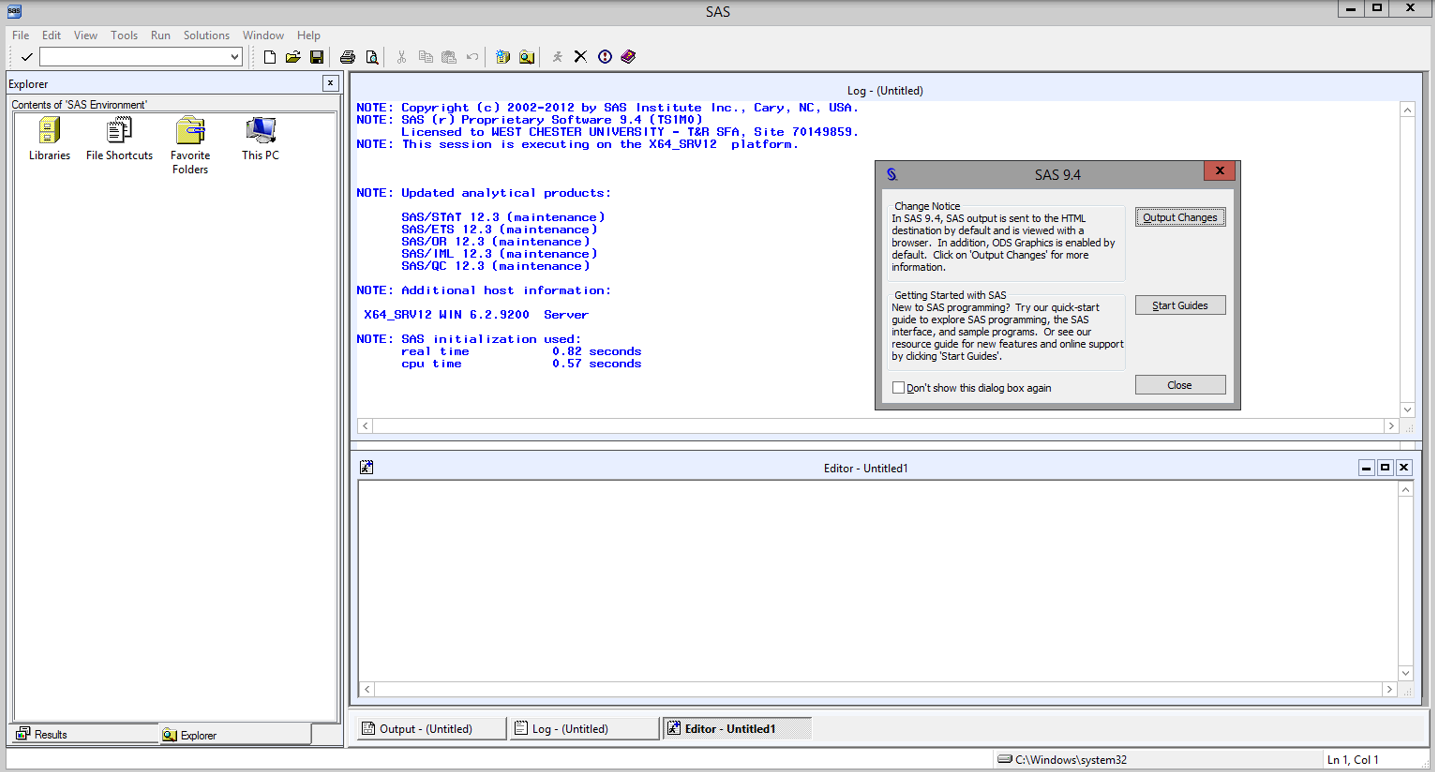
\includegraphics[width=1\linewidth]{img01/w01-SASUI} 

}

\caption{SAS use graphic interface.}\label{fig:unnamed-chunk-3}
\end{figure}

\textbf{Log Window}: It is an execution window. Here, you can check the execution of your program. It also displays errors, warnings, and notes.

\textbf{Code Window}: This window is also known as the editor window. Consider it as a blank paper or a notepad, where you can write your SAS code.

\textbf{Output Window}: As the name suggests, this window displays the output of the program/ code that you write in the editor.

\textbf{Result Window}: It is an index that lists all the outputs of programs that are run in one session. Since it holds the results of a particular session, if you close the software and restart it, the result window will be empty.

\hypertarget{sas-data-and-variables}{%
\section{SAS Data and Variables}\label{sas-data-and-variables}}

SAS data sets are also called SAS data files. A SAS data set has rows and columns. When other formats of data files such as .csv, .txt, .xls, etc., were loaded to SAS, they were converted to the SAS format data file with the extension \texttt{.sas7bdat}.

SAS has two basic types of variables: \textbf{numerical variable} and \textbf{character variable}.

\begin{itemize}
\tightlist
\item
  \textbf{Numerical variable} is the default type of variable in SAS. Mathematical expressions use numerical variables in data processing.
\end{itemize}

\textbf{Character variables} are those that are not used in mathematical expressions in variable processing.

Numerical variables can be converted into character variables if needed. But not the opposite unless the character variables are numerically encoded.

\hypertarget{sas-code-structure}{%
\section{SAS Code Structure}\label{sas-code-structure}}

\emph{SAS programming} is based on two building blocks

\textbf{DATA Step}: The DATA step creates a SAS data set and then passes the data onto a PROC step

\textbf{PROC Step}: The PROC step processes the data

\textbf{An SAS program} should follow below mentioned rules

\begin{itemize}
\item
  Almost every code will begin with either DATA or a PROC Step.
\item
  Every SAS statement ends with a semi-colon.
\item
  A SAS step ends with either RUN or QUIT.
\item
  SAS codes are not case-sensitive.
\end{itemize}

We can write a SAS statement across different lines or you can write multiple statements in one line.

\hypertarget{sas-libraries}{%
\section{SAS Libraries}\label{sas-libraries}}

\textbf{SAS library} is a collection of SAS data files that are stored in the same folder or directory on your computer or other storage such as a USB drive or a space in the cloud.

\textbf{Temporary Library}: In this library, the data set gets deleted when the SAS session ends.

\textbf{Permanent Library}: Data sets are saved permanently. Hence, they can be accessed in future SAS sessions.

Users can also create or define a new library known as user user-defined library by using the keyword \texttt{LIBNAME}. These are also permanent libraries.

\hypertarget{first-sas-code-hello-world}{%
\section{First SAS Code: ``Hello World!''}\label{first-sas-code-hello-world}}

Beginners usually start their coding with \texttt{Hello\ World!\textquotesingle{}.\ The\ SAS}Hello World` is given below.

\begin{verbatim}
/*************************************  
      My First SAS Program
       Author:  C. Peng
          Date:  08/22/2020
        Topics:  1. Data Step
                 2. Procedure Step
***************************************/

/* Data Step: Create a SAS dataset with one variable  */

DATA work.HelloWorld;            /* libname.datasetName */
  my1stSAScode = "Hello World";
RUN;

/* Procedure step: print out the SAS dataset */
PROC PRINT DATA = work.HelloWorld;
RUN;
\end{verbatim}

The above example code involves \texttt{code\ header} (information about the code), \texttt{/*\ SAS\ comments\ (usually\ multiple\ line\ comments)\ */}

\textbf{Important Notes}

\begin{enumerate}
\def\labelenumi{\arabic{enumi}.}
\item
  SAS is NOT case-sensitive! This is very different from some other case-sensitive language. When we name a variable, \texttt{VaRible} and \texttt{vaRiBlE} are identical in SAS.
\item
  A complete SAS code line MUST closed with a semi-colon (;)!
\item
  Each DATA step and PROC step MUST be closed with key word \texttt{RUN} to tell the SAS system to execute the DATA or PROC step.
\end{enumerate}

\hypertarget{sas-log-files}{%
\section{SAS Log Files}\label{sas-log-files}}

Each time a step is executed in a SAS program, SAS generates a log file. The SAS log collects messages about the processing of SAS programs and any errors that might occur. If the SAS code contains an error, the error will also be printed in the SAS log file.

\begin{figure}

{\centering 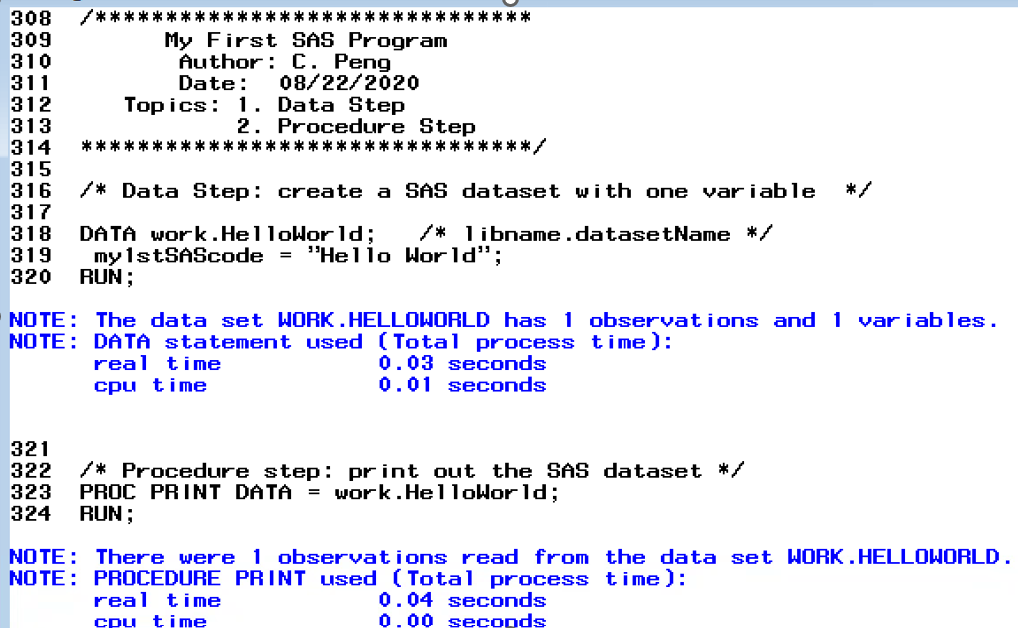
\includegraphics[width=0.7\linewidth]{img01/w01-SASLog} 

}

\caption{SAS use graphic interface.}\label{fig:unnamed-chunk-4}
\end{figure}

\hypertarget{sas-output}{%
\section{SAS Output}\label{sas-output}}

In addition to the traditional line output, the SAS 9.4 and later version allows different formats of output such as PDF, HTML, and WORD. The following screenshot shows the step of choosing HTML output.

\begin{figure}

{\centering 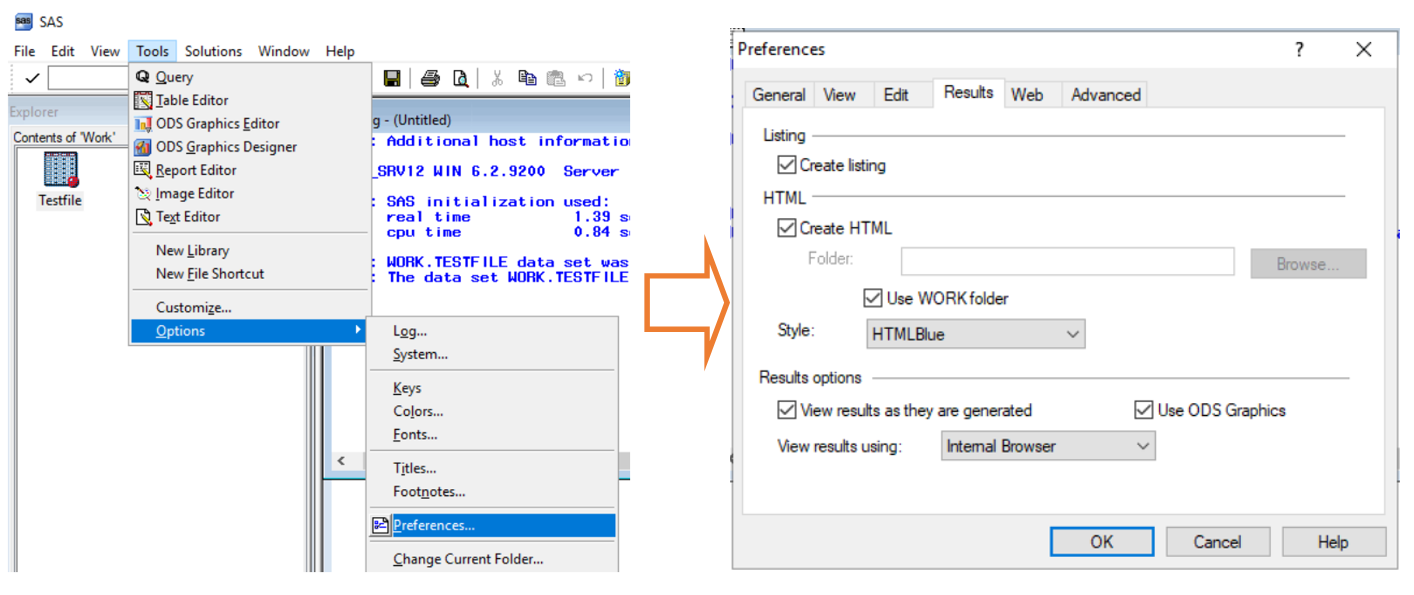
\includegraphics[width=1\linewidth]{img01/w01-ChoosingOutputFormat} 

}

\caption{Choosing SAS output formats.}\label{fig:unnamed-chunk-5}
\end{figure}

\hypertarget{some-sas-tutorial-from-sas-inc.}{%
\section{Some SAS Tutorial from SAS Inc.}\label{some-sas-tutorial-from-sas-inc.}}

\hypertarget{description-of-the-sas-program}{%
\subsection{Description of the SAS Program}\label{description-of-the-sas-program}}

\hypertarget{sas-graphical-user-interface}{%
\subsection{SAS Graphical User Interface}\label{sas-graphical-user-interface}}

\hypertarget{writing-sas-code}{%
\subsection{Writing SAS Code}\label{writing-sas-code}}

\hypertarget{coding-conventions-and-best-practices}{%
\chapter{Coding Conventions and Best Practices}\label{coding-conventions-and-best-practices}}

This chapetr discuss best practices and conventions in SAS programming. Some of the concepts covered in the previous chapter will be reviewed with more details.

\hypertarget{sas-file-and-program-structures}{%
\section{SAS file and Program Structures}\label{sas-file-and-program-structures}}

SAS data files are stored in a SAS library that is a \texttt{folder} in the directory.

\begin{figure}

{\centering \includegraphics[width=0.5\linewidth]{img02/w02-libref01} 

}

\caption{Structure of a SAS library.}\label{fig:unnamed-chunk-6}
\end{figure}

There several types of libraries in the SAS system. Temporary libraries, SAS system defined permanent libraries, and user defined permanent libraries. All data files stored in the temporary library (library reference name: \texttt{work.}) will be wiped out from the temporary library. All data files stored in the permanent libraries can be re-used in the future SAS sessions.

\begin{figure}

{\centering \includegraphics[width=0.5\linewidth]{img02/w02-libref02} 

}

\caption{Different SAS libraries.}\label{fig:unnamed-chunk-7}
\end{figure}

When we submit the LIBNAME statement, a connection is made between a \texttt{libref} in SAS and the physical location of files on the operating system.

\begin{figure}

{\centering \includegraphics[width=0.5\linewidth]{img02/w02-libref03} 

}

\caption{Naming convention of SAS library reference name.}\label{fig:unnamed-chunk-8}
\end{figure}

\hypertarget{naming-conventions-and-sas-program-structure}{%
\section{Naming Conventions and SAS Program Structure}\label{naming-conventions-and-sas-program-structure}}

Every language has its own naming conventions. The following are naming conventions in SAS programming.

\begin{itemize}
\tightlist
\item
  Every SAS statement ends in a semicolon \texttt{(;)}!!!!!!!!
\item
  All variable and data set names must start with a letter or an underscore \texttt{(\_)}.
\item
  Names can contain only letters, numerals, and the underscore. No \texttt{\%\$!*\&\#@}.
\item
  SAS is case insensitive (e.g Body, body, boDY and BoDy are all the same name to SAS).
\item
  There are no restrictions on where in the line statements start or stop and commands may be wrapped onto multiple lines.
\item
  All variable and data set names must be thirty-two (32) or fewer characters in length (8 characters in SAS V6.12 or lower).
\end{itemize}

The names \texttt{\_N\_}, \texttt{\_ERROR\_}, \texttt{\_FILE\_}, \texttt{\_INFILE\_}, \texttt{\_MSG\_}, \texttt{\_IORC\_}, and \texttt{\_CMD\_} are reserved for the variables that are generated automatically for a DATA step.

Note that SAS products use variable names that start and end with an underscore; it is recommended that we do not use names that start and end with an underscore in SAS programming.

SAS programs (scripts) are composed of DATA block and ROCedure Blocks.

\begin{figure}

{\centering 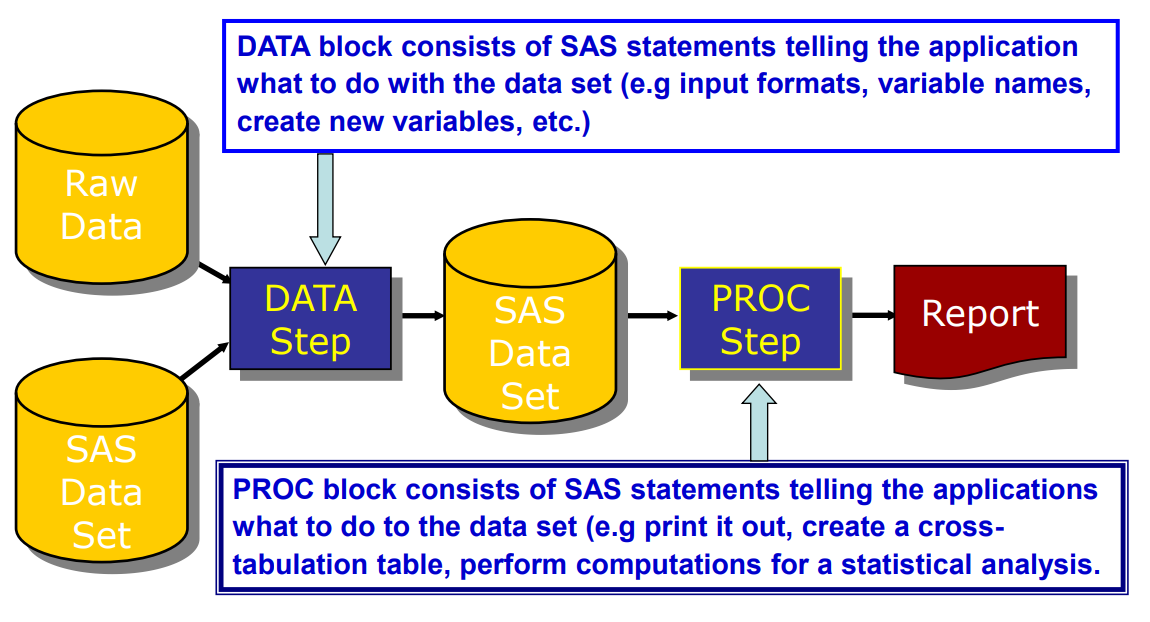
\includegraphics[width=0.5\linewidth]{img02/w02-SASCodeStructure} 

}

\caption{Naming convention of SAS library reference name.}\label{fig:unnamed-chunk-9}
\end{figure}

\begin{itemize}
\item
  \textbf{DATA block} consists of SAS statements telling the application what to do with the data set (e.g, input formats, variable names, create new variables, etc.)
\item
  \textbf{PROC block} consists of SAS statements telling the applications what to do to the data set (e.g, print it out, create a cross-tabulation table, perform computations for a statistical analysis.
\end{itemize}

\begin{figure}

{\centering 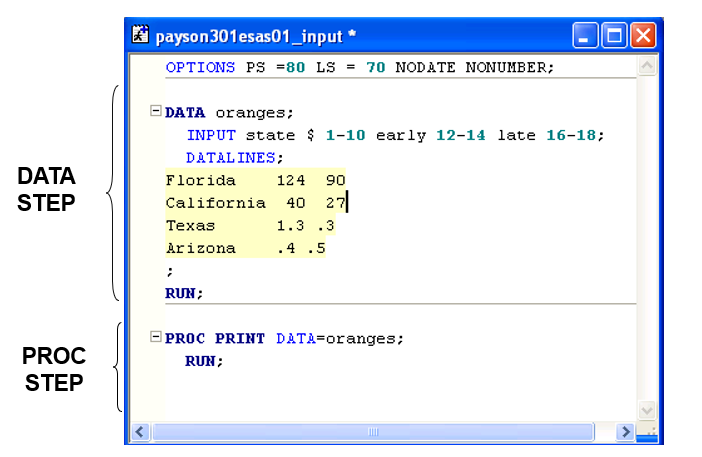
\includegraphics[width=0.5\linewidth]{img02/w02-SASEditorWindow} 

}

\caption{SAS code blocks (structure).}\label{fig:unnamed-chunk-10}
\end{figure}

After we ran the code, we should \textbf{always} check the log window for potential errors, warning messages, etc. before check the result window (line output) and \textbf{justify} the result. The following the screenshot illustrates the process.

\begin{figure}

{\centering 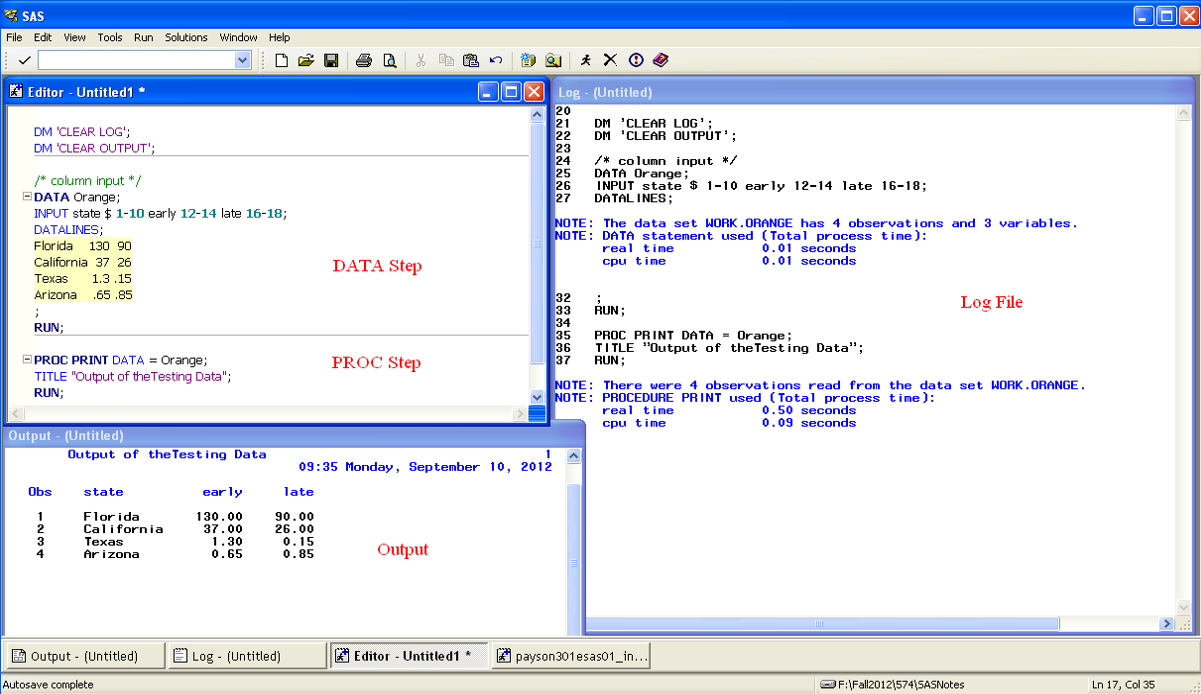
\includegraphics[width=0.9\linewidth]{img02/w02-3Windows} 

}

\caption{Basic SAS debugging process.}\label{fig:unnamed-chunk-11}
\end{figure}

\hypertarget{sas-data-structure}{%
\section{SAS Data Structure}\label{sas-data-structure}}

A SAS data set has two components: descriptor portion and data portion.

\textbf{The descriptor portion} of a SAS data set contains general information about the SAS data set (such as data set name and number of observations) variable attributes (name, type, length, position, informat, format, label).

We can use PROC CONTENTS to view the information in the data descriptor. We can add this type of information when we define a SAS data set.

The formation of formats and informats of SAS variables is carried in the data set. We next briefly describe the concepts of \textbf{formats} and \textbf{informats}:

\textbf{Informats} is used to tell SAS \textbf{how to read} a variable whereas \textbf{Formats} is used to tell SAS \textbf{how to display or write} values of a variable.

\textbf{Informats} is basically used when you read or import data from either an external file (Text/Excel/CSV) or read in sample data which was created using CARDS/DATALINES statement. It is also used when you create a new variable in a data set.

\textbf{Formats} can be used in both DATA Steps and PROC Steps whereas I\textbf{nformat} can be used only in DATA Steps.

\hypertarget{some-best-coding-practices}{%
\section{Some Best Coding Practices}\label{some-best-coding-practices}}

The following are some best practices you should always have in mind when you make a program

\begin{itemize}
\tightlist
\item
  Write a clear program header;
\item
  Write comments and documentation;
\item
  Use consistent indentation;
\item
  Don't repeat yourself (aka DRY principle);
\item
  Avoid deep nesting;
\item
  Limit line length;
\item
  Set up a simple and clear file and folder structure;
\item
  Follow naming convention;
\item
  Keep the code simple!
\item
  Save the code a version number -- version control;
\item
  Never modify the source data!!!
\end{itemize}

\hypertarget{learning-sas-coding-by-examples}{%
\section{Learning SAS Coding by Examples}\label{learning-sas-coding-by-examples}}

\begin{verbatim}
/******************************************************
    Author: C. Peng
    Date: 02/01/2021
    Updates: Fall 2020, Spring 2021
    Topics: Examples Illustrating the Following Concepts
      1. Program header;
      2. Display control;
      3. SAS display management: DM-statement
      4. SAS library - file/folder structure;
      5. Data Step and Procedure Step;
      6. Commenting and documentation;
      7. Conventions and naming rules;
      8. Debugging code - understand SAS log;
      9. Find SAS dataset structure: descriptor and data block
**********************************************/


*OOOOOOOOOOOOOOOOO;
**    Topic 1;
*OOOOOOOOOOOOOOOOO;
/*  Display management: clear log and output 
    The following DM statement will automatically
    delete the content in the designated window!
*/
DM "CLEAR LOG";
DM "CLEAR OUT";


*OOOOOOOOOOOOOOOOOOO;
**      Topic 2;
*OOOOOOOOOOOOOOOOOOO;
************************************************* 
  Set up a SAS library and save the created SAS
  dataset to the local computer - SAS permanent data
**************************************************;
LIBNAME sta311 "I:\Desktop\cpeng\WCU-Teaching\2020Fall\STA311\SAS";
   *NOTE: if you have SAS installed on your own computer,
          the path in the libname statement should be:
          LIBNAME sta311 "C:\STA311\Fall2020";


*OOOOOOOOOOOOOOOOOO;
**   Topic 3;
*OOOOOOOOOOOOOOOOOO;
/**************************************************************
  Display control: SAS system OPTIONS
  There many options avaialble in SAS that can be found by typing
  PROC OPTIONS; 
  RUN;
  Most commonly used options are:
  pagesize, linesize, date, nodate, number, nonumber, etc. See SAS
  document for explanantions of these commonly used options:
  https://documentation.sas.com/?docsetId=basess&docsetTarget=n1km315k2himgpn1j6d82y0yju4v.htm&docsetVersion=9.4&locale=en
***************************************************************/
OPTIONS PS = 100  /* page size of log and output (listing) */
        LS = 90   /* line size of log and output (listing) */   
        NODATE    /* turn off the date option in listing window */
        NONUMBER; /* SAS will not print page numbers in the output window */


*OOOOOOOOOOOOOOOOO;
**    Topic 4; 
*OOOOOOOOOOOOOOOOO;
/*********************************************
 DATA step statements
 One way to create SAS dataset is to use DATA step
 statement. There are several different ways to read 
 data in different formats. We will introduce the three
 most commonly used methods: column, list, and formatted
 methods. The following DATA step uses the column input.

 Components of a DATA STEP:

 DATA statement;
 INPUT statement;
 DATALINES (CARDS);
    data block
        ;
 RUN statement;

 The different input styles determine the types of input.
 The detailed information can be found at
 https://documentation.sas.com/?docsetId=lestmtsref&docsetTarget=n0oaql83drile0n141pdacojq97s.htm&docsetVersion=9.4&locale=en#p0ert9pwdtsq4en1czu9tcrncgm8

 Column input illustration:
----+----1----+----2----+----3----
Florida    130 90


**********************************************/
/* This data step uses COLUMN INPUT style, More examples
    and explanations will be given in the next few weeks.
*/

DATA Orange;  /* send the SAS data set to the temporary library */        
INPUT state $ 1-10 early 12-14 late 16-18; 
     /*
     SAS has two basic types of data: numeric and categorical. $ is used 
     to specify categorical data. As an example, we look at variable state:
     $ indicates that state is a categorical variable.
     1-10: all characters including white space in the first column define 
           a string. That string is the value of the categorical variable STATE.     
     */

/* DATALINES - tells SAS the data block begins.
   we can also use CARDS instead. CARDS was used
   in the old version of SAS.                 */
DATALINES; 
Florida    130  90
California  37  26
Texas      1.3 .15
Arizona    .65 .85
;     /* this semi-colon is required! SAS will wait for
         the next line of data until "seen" this semi-colon.*/
RUN;  /* This is optional, but it is always a good idea to
         close this DATA STEP with this RUN; statement.     */

/*  Follow the steps to see where this data SAS data resides:
    go to the Explore window -> Libraries -> Work -> Orange
*/


*OOOOOOOOOOOOOOOOOO;
**     Topic 5;
*OOOOOOOOOOOOOOOOOO;
/******************************************************
A simplest SAS Procedure syntax:

PROC keyword DATA = datasetname;
 the specific task to perform on a SAS data set;
RUN;

Next, we print out the SAS data set created from the above 
DATA STEP
*******************************************************/

PROC PRINT DATA = Orange; /* PRINT <- keyword, DATA <- dataset in the trmporary library */
TITLE1 "This is a toy data set";
TITLE2 "Orange";
RUN;

/* After you run this block of code, you will see the data set
   in a browser (html) and the output window (if it is selected).  */

** Topic 6. SAS data structure: descriptor;
/* We can find descriptor of as SAS data set by using PROC CONTENTS */

PROC CONTENTS DATA = ORANGE; /* display the contents in the output windows */
RUN;

/* Remarks: The default length for a numeric variable is 8 bytes. 
   The length of a character variable is set at the first occurrence of the variable.

   The following data step is called LIST INPUT. More examples and details 
   will be given in the next few weeks.
*/

DATA Orange_02;  /* send the SAS data set to the temporary library */        
INPUT state $  early   late  ; 
DATALINES; 
California  37  26
Florida    130  90
Texas      1.3 .15
Arizona    .65 .85
;
RUN;

PROC PRINT DATA = ORANGE_02;
TITLE1 "List input style";
TITLE2 "Orange 02";
RUN;

TITLE "";
PROC CONTENTS DATA = ORANGE_02; /* display the contents in the output windows */
RUN;


/* You can check them out from the Results windows: */

/*OOOOOOOOOOOOOOOOOOOOOOOOO
         Summary
OOOOOOOOOOOOOOOOOOOOOOOOOOO

1. A good program should have an informative program header.
2. Define a library to store your SAS data sets. 
3. Set options to produce nice-looking outputs.
4. Commenting on your program to make it clear and understandable.
5. DATA step creates and/or modifies SAS data sets.
6. PROC step performs specific tasks on SAS data.

Next time, we still use column input to define the data set and add 
a few more ingredients in both the data step and procedure step to make 
better SAS programs.

*******************************/
\end{verbatim}

\hypertarget{methods-of-sas-data-input}{%
\chapter{Methods of SAS Data Input}\label{methods-of-sas-data-input}}

Before we introduce SAS input methods, we first review the basic concepts introduced previously.

\textbf{SAS Data Set} - a binary formatted representation of the input data set stored in such a way that future SAS programs do not need to input the data again.

\textbf{Temporary SAS Data Sets} - created and remain in working memory for the SAS session, but disappear when the SAS session ends. It is fine for small to moderate-sized, simple input programs.

\textbf{Permanent SAS Data Sets} - created in one SAS session but stored on disk for later reuse. It is convenient for large or complex input data sets that may require multiple analysis steps. It reduces time and computer resources.

\textbf{LIBNAME statement} - identifies the SAS program where the previously created SAS data set is located.

\textbf{Use of Comments} - to make the code easy to understand. The purpose of comments is

\begin{itemize}
\item
  To note the history of your analysis.

  \begin{itemize}
  \tightlist
  \item
    Keep track of the steps you took to create the data set.
  \item
    Keep track of data modifications.
  \item
    Keep track of all statistical analyses attempted.
  \end{itemize}
\item
  Assist others in understanding your analysis.
\item
  To block out sections of the program ( \texttt{/*} and \texttt{*/}) allowing you to run partial analyses but return to previous analyses if you change your approach.
\item
  To refresh your memory about the project you have to return to the analysis to answer questions from Journal reviewers, academic advisers, and colleagues, months or years after the data have been analyzed.
\end{itemize}

\hypertarget{specifying-variable-length}{%
\section{Specifying Variable Length}\label{specifying-variable-length}}

One of the important pieces of information in data input is to specify the length of each input variable. This is also one of the sources of common errors in data input. Here is some important information about the lengths of SAS variables.

\begin{itemize}
\item
  The default length for character and numeric variables is 8 bytes in SAS.
\item
  SAS uses exactly one byte for one character! This means that if the value of a character variable has more than 8 characters, SAS only keeps the first 8 characters (including the white space if any) and truncates the rest.
\item
  However, for a numeric variable SAS variable, 8 bytes can store a number with up to 16 digits. In other words, the default length of a numeric variable is 16 digits.
\item
  It is important to note that the minimum length of a numeric is 3 bytes. It does not mean it cannot store a numeric value lower than 3 digits. It can store values of 1 or 2 digits.
\item
  The maximum length of any character value in SAS is 32,767 bytes!
\end{itemize}

\textbf{Specifying the length of variables}

Variable lengths specified in a LENGTH statement affect the length of numeric variables only in the output data set; during processing, all numeric variables have a length of 8 bytes.

Lengths of character variables specified in a LENGTH statement affect both the length during processing and the length in the output data set.

\begin{figure}

{\centering 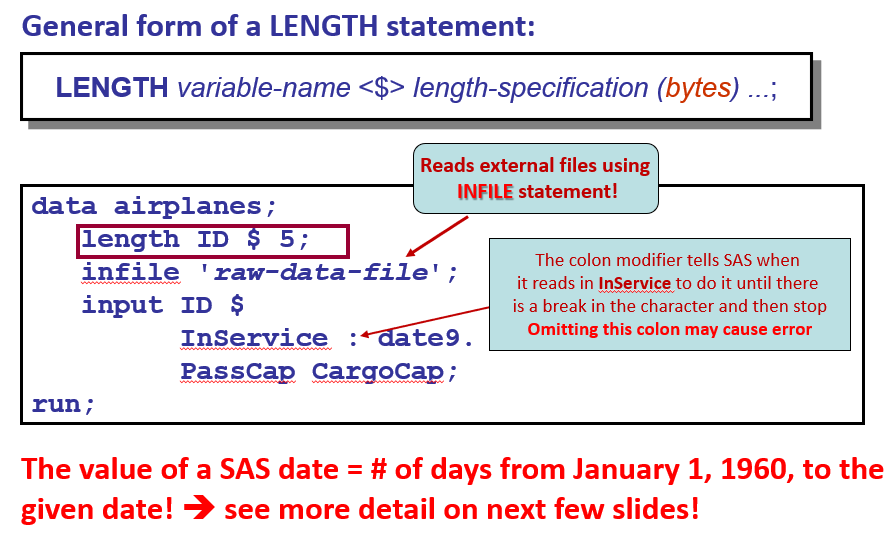
\includegraphics[width=0.6\linewidth]{img03/w03-SpecifyingLengthofVariables} 

}

\caption{Specifying length of input variables.}\label{fig:unnamed-chunk-13}
\end{figure}

Don't forget to use the dollar sign \texttt{\$} when specifying the length of a character variable. See the following figure.

\begin{figure}

{\centering 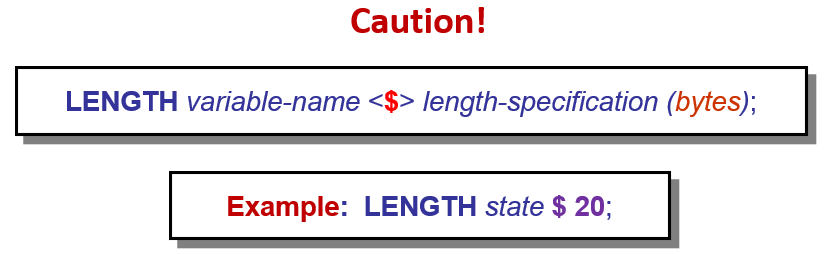
\includegraphics[width=0.6\linewidth]{img03/w03-SpecifyingLengthofChar} 

}

\caption{Caution about specifying length of character variables..}\label{fig:unnamed-chunk-14}
\end{figure}

\hypertarget{methods-of-data-input}{%
\section{Methods of Data Input}\label{methods-of-data-input}}

Three basic input styles in SAS are illustrated in the following figures.

\hypertarget{list-input}{%
\subsection{List Input}\label{list-input}}

The input data values are simple and the default length of variables are used. Dollar signs are also used to specify the character variables in the data set.

\begin{figure}

{\centering 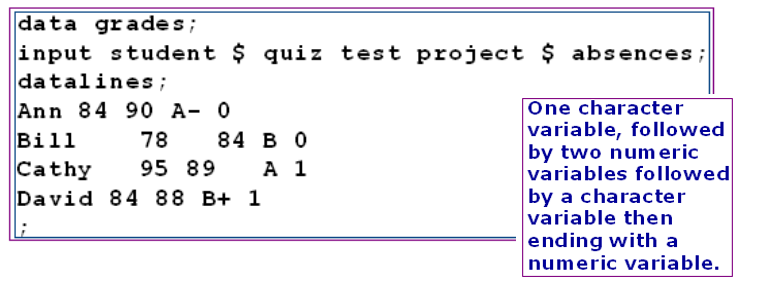
\includegraphics[width=0.6\linewidth]{img03/w03-LinrInput} 

}

\caption{SAS data input styles.}\label{fig:unnamed-chunk-15}
\end{figure}

When data columns are not lined up, use list input. Make sure, the data file has the following features

\begin{itemize}
\item
  At least one blank between values of adjacent variables;
\item
  No white space (blanks) within data values; For example, \texttt{Mary\ Beth} has a white space in the character value, and list input should not be used.
\item
  Character data values must be less than or equal to 6 characters.
\end{itemize}

The above code includes the input data file in the program (also called \texttt{inline\ input}). \texttt{DATALINES} or \texttt{CARDS} statement is used for all inline input.

When the input data file is a data file in a physical location in a drive, \texttt{INFILE} statement must be used.

\hypertarget{column-input}{%
\subsection{Column Input}\label{column-input}}

With column pointers, we can tell SAS directly which column to begin reading a variable from.

\begin{itemize}
\tightlist
\item
  Go directly to the information you really need.
\item
  Skip unnecessary information.
\item
  Efficient data entry
\end{itemize}

The following figure shows column input with an external file.

\begin{figure}

{\centering 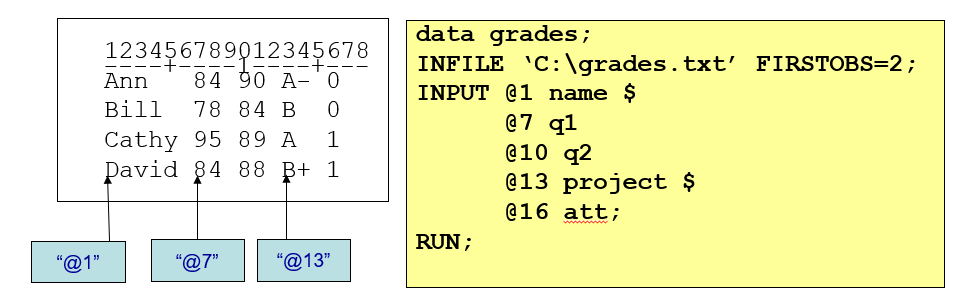
\includegraphics[width=0.6\linewidth]{img03/w03-ColumnInput} 

}

\caption{Column input with an external data file.}\label{fig:unnamed-chunk-16}
\end{figure}

\hypertarget{formatted-input-delimited-input}{%
\subsection{Formatted Input (Delimited Input)}\label{formatted-input-delimited-input}}

The fundamental difference between column input, which we studied in the previous lesson, and formatted input, which we'll explore now, is that column input is only appropriate for reading standard numeric data, while formatted input allows us to read both standard and nonstandard numeric data. That is, formatted input combines the features of column input with the ability to read nonstandard data values including

\begin{itemize}
\tightlist
\item
  values that contain special characters, such as dollar signs (\$), percent signs (\%), and commas (,)
\item
  date and time values
\item
  data in fraction, integer binary, real binary, and hexadecimal forms
\end{itemize}

\begin{figure}

{\centering 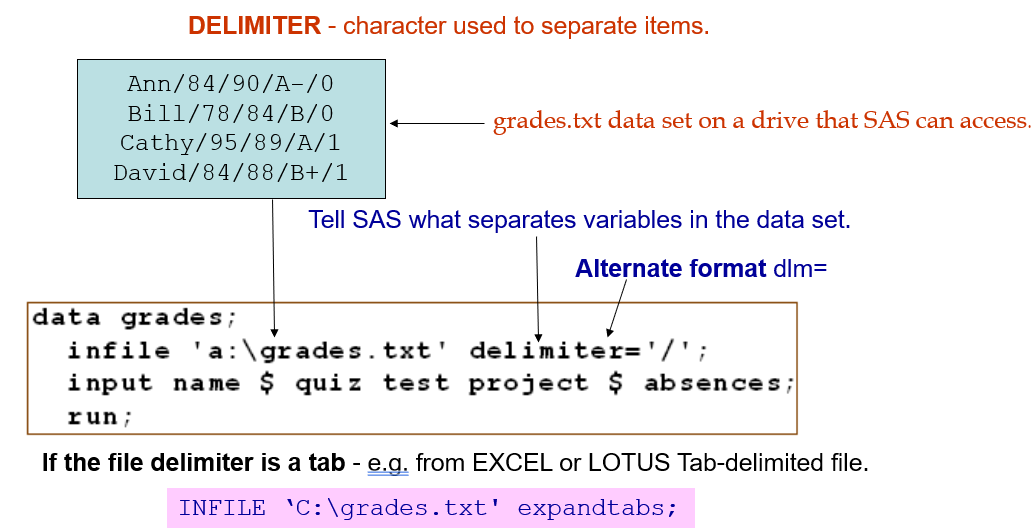
\includegraphics[width=0.65\linewidth]{img03/w03-formattedInput} 

}

\caption{Delimited (formatted) input.}\label{fig:unnamed-chunk-17}
\end{figure}

\hypertarget{summary---three-input-styles}{%
\subsection{Summary - Three Input Styles}\label{summary---three-input-styles}}

\begin{figure}

{\centering 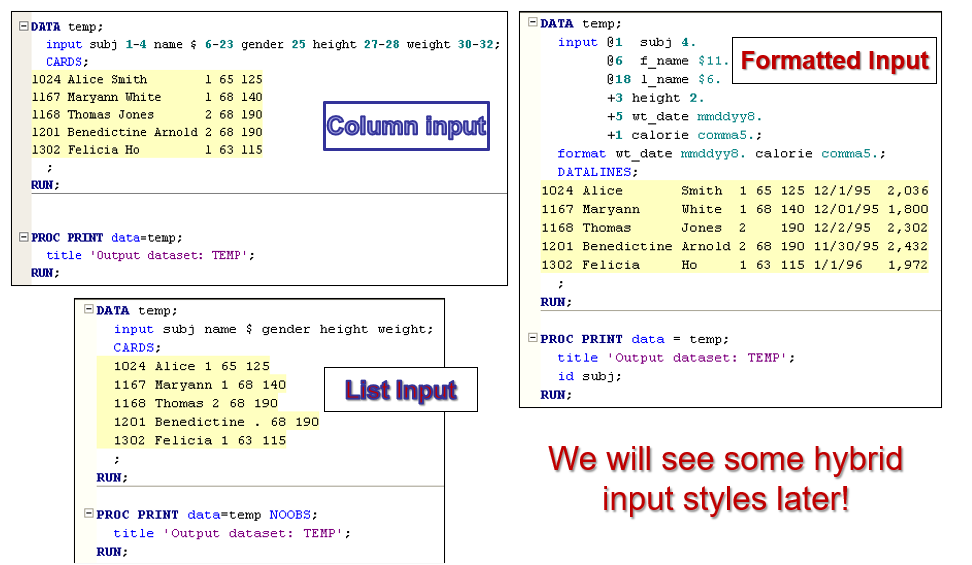
\includegraphics[width=1\linewidth]{img03/w03-3InputStyles} 

}

\caption{SAS data input styles.}\label{fig:unnamed-chunk-18}
\end{figure}

\hypertarget{mixed-input}{%
\subsection{Mixed Input}\label{mixed-input}}

SAS also allows mixed input. The following figure gives an example that involves mixed input styles.

\begin{figure}

{\centering 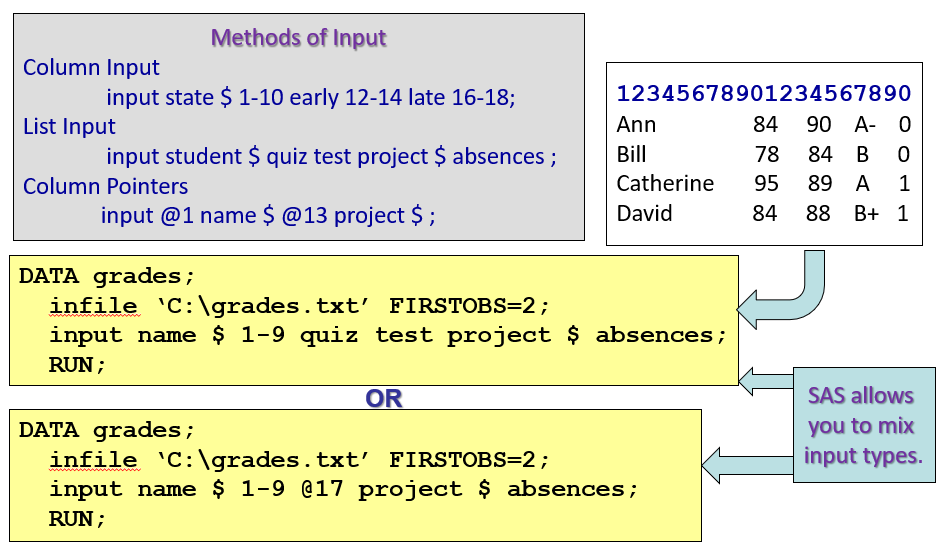
\includegraphics[width=0.85\linewidth]{img03/w03-MixedInput} 

}

\caption{Mixed input style.}\label{fig:unnamed-chunk-19}
\end{figure}

\hypertarget{handling-special-structured-data}{%
\section{Handling Special Structured Data}\label{handling-special-structured-data}}

Sometimes, the input data files may have different structures, we need special handling of these types of data layouts.

\hypertarget{data-file-containing-comments-and-descriptions}{%
\subsection{Data File Containing Comments and Descriptions}\label{data-file-containing-comments-and-descriptions}}

We can use keywords \texttt{FIRSTOBS\ =} and

\begin{figure}

{\centering 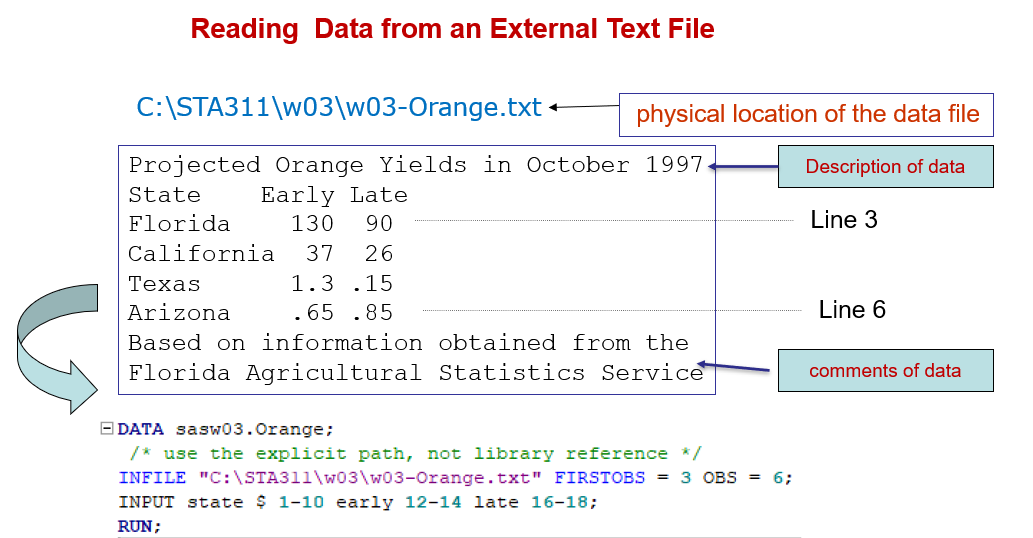
\includegraphics[width=0.8\linewidth]{img03/w03-readInExternalTextFiles01} 

}

\caption{Data file with descriptions and comments.}\label{fig:unnamed-chunk-20}
\end{figure}

\hypertarget{multi-line-for-the-record}{%
\subsection{Multi-line for the Record}\label{multi-line-for-the-record}}

Data may come to us with each observation recorded on more than one line. We need to be able to tell SAS to go to the next line. SAS can do the trick in two different ways.

\begin{itemize}
\tightlist
\item
  The slash (/) says to skip to the next line.
\item
  The code \#n says go to that line of the observations data to resume reading data.
\end{itemize}

\begin{figure}

{\centering 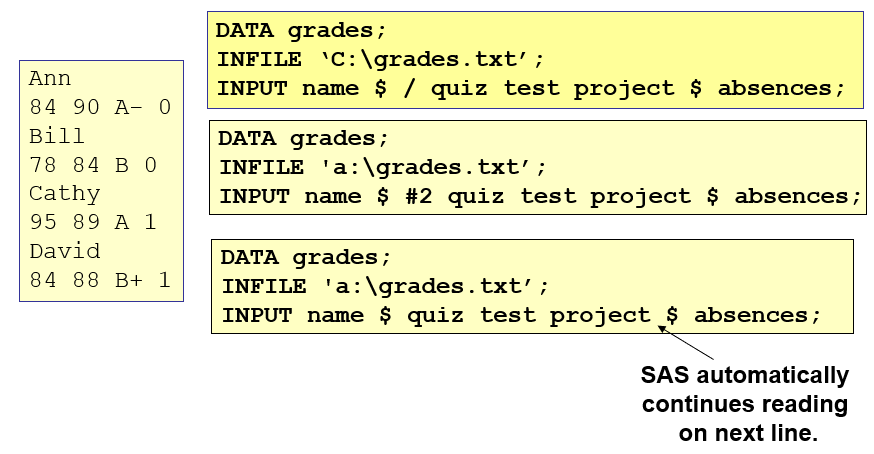
\includegraphics[width=0.8\linewidth]{img03/w03-multi-line-record} 

}

\caption{Reading in multi-line records.}\label{fig:unnamed-chunk-21}
\end{figure}

\hypertarget{multi-records-in-the-same-line}{%
\subsection{Multi-records In the Same Line}\label{multi-records-in-the-same-line}}

In case situations, we may have data sets in which a single line may have multiple records. In SAS. trailing ``at'' symbols ( \texttt{@@} ) tells SAS to hold the current data line for further information.

\begin{itemize}
\tightlist
\item
  Read in name--absences then hold the current position on the data line.
\item
  Read in another set of names--absences then hold position.
\item
  Keep doing this until an end-of-line marker is reached.
\end{itemize}

The next data step gives an example of this type of data.

\begin{verbatim}
DATA grades;
  INPUT name $ quiz test project $ absences @@;
DATALINES;
Ann 84 90 A- 0 Bill 78 84 B 0 Cathy 95 89 A 1 
David 84 88 B+ 1
;
RUN;
\end{verbatim}

\hypertarget{making-better-line-outputs}{%
\section{Making Better Line Outputs}\label{making-better-line-outputs}}

We view the results line output window frequently in analysis. There are different ways that we can use to make the output better looking and more informative.

\hypertarget{options-statement}{%
\subsection{OPTIONS Statement}\label{options-statement}}

\textbf{OPTIONS Statement} is placed at the beginning of the program to control output options. It remains in effect until you change it. The commonly used options are given in the following figure.

\begin{figure}

{\centering 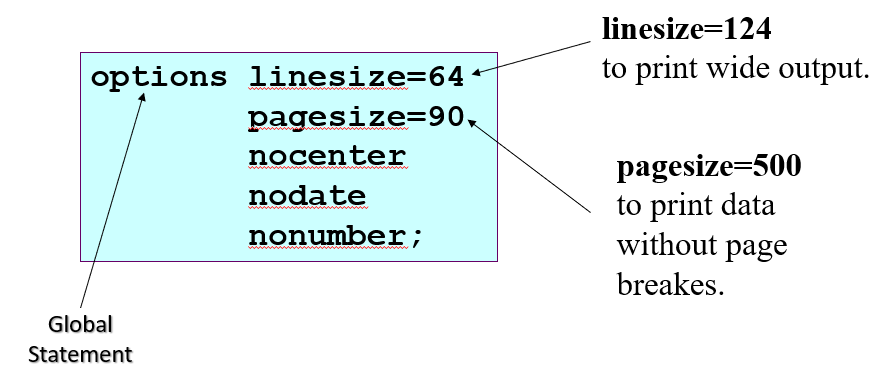
\includegraphics[width=0.6\linewidth]{img03/w03-GlobalOptions} 

}

\caption{Global options of output.}\label{fig:unnamed-chunk-22}
\end{figure}

\hypertarget{titles-and-footnotes}{%
\subsection{Titles and Footnotes}\label{titles-and-footnotes}}

Use a TITLE and/or FOOTNOTE statement to place comment information at the top (TITLE) or bottom (FOOTNOTE) of each output page.

Once set, TITLE and FOOTNOTE information will be printed for each procedure output unless a new TITLE or FOOTNOTE statement is encountered.

\begin{figure}

{\centering 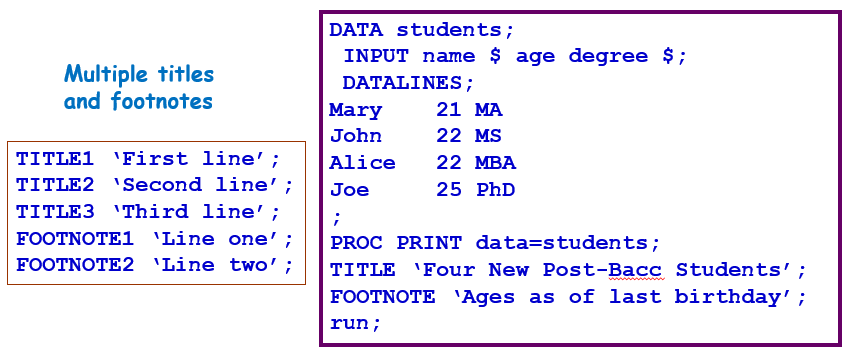
\includegraphics[width=0.6\linewidth]{img03/w03-TitlesFootnotes} 

}

\caption{Titles and footnotes.}\label{fig:unnamed-chunk-23}
\end{figure}

\hypertarget{labeling-variables}{%
\subsection{Labeling Variables}\label{labeling-variables}}

We use the label statement in the data step to assign labels to the variables. We could also assign labels to variables in proc steps, but then the labels only exist for that step. When labels are assigned in the data step they are available for all procedures that use that data set.

To explain, we first define a data set.

\begin{verbatim}
DATA auto ;
  INPUT make $  mpg rep78 weight foreign ;
DATALINES;
AMC     22 3 2930 0
AMC     22 . 2640 0
Audi    17 5 2830 1
Audi    23 3 2070 1
BMW     25 4 2650 1
Buick   26 . 2230 0
Buick   19 3 3400 0
Cad.    14 3 4330 0
Cad.    14 2 3900 0
Cad.    21 3 4290 0
Chev.   29 3 2110 0
Chev.   19 3 3430 0
Datsun  23 4 2370 1
Datsun  35 5 2020 1
;
RUN;
\end{verbatim}

The following program assigns variable labels to rep78, mpg, and foreign.

\begin{verbatim}
DATA  auto2;
   SET auto;
   LABEL  rep78  ="1978 Repair Record"
          mpg    ="Miles Per Gallon"
          foreign="Where Car Was Made";
RUN;
\end{verbatim}

You can see the labels in the PROC CONTENTS procedure.

\hypertarget{formats-and-user-define-formats}{%
\subsection{Formats and User Define Formats}\label{formats-and-user-define-formats}}

Sometimes, people also consider labels as a kind of format. SAS has many different formats for special variables, for example, SAS date formats. SAS also allows users to define formats. The next example shows how to define formats for variables.

\begin{verbatim}
PROC FORMAT;
  VALUE  forgnf 0="domestic"
                1="foreign" ;
                
  VALUE  $makef "AMC"    ="American Motors"
                "Buick"  ="Buick (GM)"
                "Cad."   ="Cadillac (GM)"
                "Chev."  ="Chevrolet (GM)"
                "Datsun" ="Datsun (Nissan)";
RUN;
\end{verbatim}

It should be noted that a dollar sign \texttt{\$} must be used when defining a format for a character variable! Once a format of a variable is defined, it will be used the same way as other built-in formats in SAS to make better output.

\hypertarget{a-note-on-sas-dates}{%
\subsection{A Note on SAS Dates}\label{a-note-on-sas-dates}}

SAS dates are complex in format. We will not discuss this systematically here. When the SAS date is a numerical variable, its value is the number of days since 1/1/1960. That is, 1/1/1960 00:00:00 is set as ZERO.

\begin{figure}

{\centering 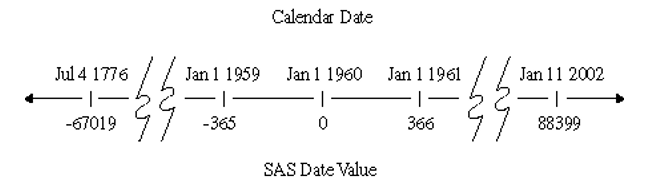
\includegraphics[width=0.6\linewidth]{img03/w03-SAS-Date-Def} 

}

\caption{Determination of SAS date values.}\label{fig:unnamed-chunk-24}
\end{figure}

\hypertarget{learning-sas-coding-by-examples-1}{%
\section{Learning SAS Coding by Examples}\label{learning-sas-coding-by-examples-1}}

This section gives several examples of SAS code with comments on some coding specifics.

\begin{verbatim}
/*******************************************************************************
         Topics: 1. Review: SAS display management, library, options, 
                    permanent/temporary data set 
                 2. SAS INPUT styles: column input, list input, formatted input;
                 3. Variable LENGTH specification
                 4. INFILE - reading external data file
                 5. SAS Labels
                 6. SAS informat/format
*******************************************************************************/

/**********************************
1. Review: Options, LIBNAME, DM
***********************************/
OPTIONS NODATE NONUMBER PS = 80 LS = 64 nodate nonumber;   * to specify the form of sas output;
LIBNAME  sasw03  'C:\STA311\w03';          * permenent library;

/* clear log and output windows */
DM 'CLEAR LOG';
DM 'CLEAR OUTPUT';


/***************************************************
 2. SAS INPUT styles: column, list, and formats
****************************************************/


/* 2.1. column input with inline data - values of variables must be 
        placed within the corresponding range and values of adjacent
        variables must separated by at least one blank.           */
DATA Orange;
INPUT state $ 1-10 early 12-14 late 16-18;   
DATALINES;
Florida    130  90
California  37  26
Texas      1.3 .15
Arizona    .65 .85
;
RUN;

PROC PRINT DATA = Orange;
TITLE "Output of the testing Data";
RUN;

/**------- key takeaways -------
1. flag character variable with $
2. INPUT statement: Specify variable type and length.
3. TITLE is a global statement. To delete the previous title, 
   use statement TITLE ""; 
4. TITLE can be placed either inside PROC or outside PROC.
---------------------------*/

/* 2.2. List input  */
DM 'CLEAR LOG';
DM 'CLEAR OUTPUT';

/* List input - No blanks between the values of character variables 
                values between adjacent variables must be separated 
                by at least one blank.                         */
DATA Orange_list;
LENGTH state $ 10.;
INPUT state $ early late;
DATALINES;
Florida    130  90
California  37  26
Texas      1.3 .15
Arizona    .65 .85
;
RUN;

PROC PRINT DATA = orange_list;
TITLE 'Include data values in the sas program';
RUN;

/*--------- Key Takeaways  ----------------------------------------------------------------
1. A list is appropriate when no blanks are in the values of the character variable.
2. If the maximum length of the character variable value is bigger than 8 (i.e., more than
   8 characters including blanks BETWEEN the strings, we need to define the length 
   of the variable using the statement: LENGTH char_name $ specified-length
3. One can also specify the length within the INPUT statement: char_name $ specificed_length.
   Example, INPUT State_name $ 18.;
--------------------------------------------------------------------------------------------*/


/********************************************************
  2.3. column pointer-formatted input - 
       values of all variables must be placed
       within the corresponding column range. 
       There is NO need to separate the values
       of adjacent variables in column pointer input. 
**********************************************************/
DM 'CLEAR LOG';
DM 'CLEAR OUTPUT';

DATA kids;
  INPUT @1 firstnam $ 11.     /* @ <== column pointer  */
        @12 lastname $11.    /* $ <== char variable indicator */
        @23 birthday $10.    /* in $10, 10 <== length of birthday  */
        @ 33 gender $1.       /* @33  33 <== value of gender starts at column 33  */
        @34 wklyrate;        /* close the INPUT statement with a semi-colon. */
DATALINES;                     
Douglas    Lindgren   08/29/1996M115
Elizabeth  Wilkerson  01/13/1997F95
Evangeline Chambers   03/11/1997F100
Arthur     Hollander  07/19/1996M.
ChristopherKalbfleisch04/13/1995M115
Stacy      Siegel     11/15/1996F100
;
RUN;

PROC PRINT DATA =kids;
 TITLE 'Daycare roster';
RUN;

/*-------------------- Key Takeaways  -------------------
1. In INPUT statement, a column pointer must be placed in 
    front of the corresponding variable.
2. length-specifier: $20 and $ 20 both work fine!
3. column pointer: @33 and @ 33 both work fine!
---------------------------------------------------------*/


/******************************************************************
 3. INFILE - specify whether part of whole of an inline external
             data file should be read into SAS.
*******************************************************************/

DM 'CLEAR LOG';
DM 'CLEAR OUTPUT';

LIBNAME  sasw03  'C:\STA311\w03';          * permenent library;


/* 3.1 read in part of an external data file */
DATA sasw03.Orange;
INFILE "C:\STA311\w03\w03-Orange.txt" FIRSTOBS = 3 OBS = 6;  /* use the explicit path, not library reference, 
                                                                The input data is NOT as SAS format data set!*/
INPUT state $ 1-10 early 12-14 late 16-18;
RUN;

/*---------------  Key Takeaways  -------------------
1. FIRSTOBS = 3: <== Start reading data from row 3. 
  (The first 2 rows contain data descriptions)
2. OBS = 6:  <== the last row to read in SAS. (The rest
   of the rows are part of the data file).
3. INPUT is used as usual to tell the information of the variables!
4. INFILE statement tells the location of the data file. 
   For an external file, the path to the file must be given. FIRSTOBS
   and OBS are optional.
----------------------------------------------------*/

PROC PRINT DATA = sasw03.Orange;
TITLE 'Read in data from an external data file';
RUN;
QUIT;


DM 'CLEAR LOG';
DM 'CLEAR OUTPUT';


/* 3.2. inline text data with descriptions - read part of the data file: 
        FIRSTOBS=  OBS =  */
DATA Inline_Orange;
INFILE DATALINES FIRSTOBS = 3 OBS = 6;
INPUT state $ 1-10 early 12-14 late 16-18;
DATALINES;
Projected Orange Yields in October 1997
State    Early Late
Florida    130  90
California  37  26
Texas      1.3 .15
Arizona    .65 .85
Based on information obtained from the
Florida Agricultural Statistics Service
RUN;

PROC PRINT DATA =Inline_Orange;
TITLE 'Read in data from an inline data file';
RUN;
QUIT;

/*------------------ Key Takeaways  ----------------
1. DATALINES in the INFILE statement points to the location 
   of the inline data file which is below the DATALINES statement.
2. INPUT statement specifies the information of variables as usual 
   regardless of using an inline data file or an external data file.
----------------------------------------------------*/



/*****************************************************************************
 4. Complex data layout: (1). The single record was split into multiple lines;
                         (2). Multiple records were put in the sample line.
*******************************************************************************/

DM 'CLEAR LOG';
DM 'CLEAR OUTPUT';

/** 4.1 Read in specially layout data: one record in multiple lines
        In the old version of SAS, we need to use '\' or '#2' to tell SAS
        to continue to read data in the next row. In 9.0 or later, SAS
        automatically will go to the next line to read data until completing
        the record.
    **/
DATA inline_grades_multi_line;
INPUT NAME $ / QUIZ TEST PROJECT $ ABSENCES; 
DATALINES;
Ann       
84 90 A- 0
Bill   
78 84 B 0
Cathy     
95 89 A 1
David     
84 88 B+ 1
;
RUN;

PROC PRINT DATA = inline_grades_multi_line;
RUN;


/*** 4.2. External txt file - one record in multiple lines ***/
DATA grades_multi_line01;
INFILE "C:\STA311\w03\w03-multi-line-grades.txt";
INPUT NAME $ / QUIZ TEST PROJECT $ ABSENCES;
RUN;

PROC PRINT; RUN;   /* If the data set is not specified, PROC PRINT will print 
                      the most currently created SAS data set!                */


DM 'CLEAR LOG';
DM 'CLEAR OUTPUT';

/** 4.3. Multiple records in one line: double trailings: 
         @@  must be used as in the following to read the 
         data correctly in SAS.                       **/

DATA grades_multiple_obs;
  INPUT name $ quiz test project $ absences;
DATALINES;
Ann 84 90 A- 0 Bill 78 84 B 0 Cathy 95 89 A 1 
David 84 88 B+ 1
;
RUN;

PROC PRINT; RUN;


DM 'CLEAR LOG';
DM 'CLEAR OUTPUT';

/* INFILE-DATALINES combination ;   */
/* 4.4. It will create a wrong data set if '@@' is used!  */
DATA grades_infile_dataline;
INFILE DATALINES;
  INPUT name $ quiz test project $ absences;
DATALINES;
Ann 84 90 A- 0 Bill 78 84 B 0 Cathy 95 89 A 1 
David 84 88 B+ 1
;
RUN;

TITLE " grades_infile_dataline;";
PROC PRINT; RUN;
TITLE "";

/*------------------ Key Takeaways  ----------------------------
1. The types of errors that SAS log reports are related to syntax. 
   However, seeing no error in the log window does not mean
   you created a correct data set! You need to the content of the
   DATA SET before moving to the next step.
2. When you create multiple data sets, add a meaningful title 
   PROC PRINT step so you can see the clear title in each output.
   It is a good practice to CLEAR the old title for the next new title
   by typing TITLE ""; after the PROC PRINT step. 
----------------------------------------------------------------*/



/* =====================================================
 5. Review: SAS Permanent SAS library - create a permanent 
            SAS library to store SAS  *data set*!!! 
             Caution - you can save your SAS
             file to the folder you used for the SAS library 
             without using library reference!! 
========================================================= */

DM 'CLEAR LOG';
DM 'CLEAR OUTPUT';

LIBNAME SASWK3 'C:\STA311\w03';   /* Create a folder under C drive and use the
                                     environment shortcut to search the folder,
                                     the actual PATH to the folder shown on the
                                     top-left of the Explorer window. You need to
                                     type the path inside the single quote'' to
                                     define the permanent library.             */

/** 5.1 Save the created SAS data set to the permanent SAS library  **/
DATA SASWK3.libname_orage;
LENGTH state $ 10.;
INPUT state $ early late;
DATALINES;
Florida    130  90
California  37  26
Texas      1.3 .15
Arizona    .65 .85
;
RUN;

PROC PRINT DATA = SASWK3.libname_orage;
TITLE 'Print the  libname_ permanent data set';
RUN;


/* ====================================================
 6.     Label and Informat/Format

      It is very important to attach as much information 
      as possible to the variables. Useful information
      includes

    - LABEL: a description or definition of variables
      in the SAS data set. 
    - INFORMAT: Tell SAS the format of the input variables
    - FORMAT: Tell SAS the format you want to display in the
              SAS output.
========================================================*/

/*****************************************************
5.1. Label - it describes each input variable
             This information will be kept in the resulting 
             SAS data set. Most importantly, this information
             will be carried over to the SAS data sets derived
             from the initial data set.
******************************************************/
DM 'CLEAR LOG';
DM 'CLEAR OUTPUT';
DATA kids_label;
  INPUT @1 firstnam $11. 
        @12 lastname $11.
        @23 birthday $10. 
        @33 gender $1. 
        @34 wklyrate 3.;
  LABEL firstnam='First name' 
        lastname='Last name'
        birthday='Birthday in days from Jan. 1, 1960' 
        gender='Gender'
        wklyrate='Rate';
DATALINES;
Douglas    Lindgren   08/29/1996M115
Elizabeth  Wilkerson  01/13/1997F95
Evangeline Chambers   03/11/1997F100
Arthur     Hollander  07/19/1996M.
ChristopherKalbfleisch04/13/1995M115
Stacy      Siegel     11/15/1996F100
;
RUN;

PROC PRINT DATA =kids_label;
 TITLE 'Daycare roster: kids Label';
RUN;


/*******************************************************************
5.2. SAS Date Informat/Format

About SAS Dates:

1. A SAS date is saved as a numeric value
  that represents the number of days since
  January 1, 1960. A negative value implies
  that the date is earlier than January 1, 1960.
  A positive value means the date is after January 1, 1960.

2.FORMAT: If you want to display a date, you need to
  specify a format. Otherwise, you will have a numerical
  value. There are many different formats for dates in SAS.
  See the following link to the SAS document:
  https://documentation.sas.com/?docsetId=lrcon&docsetTarget=p1wj0wt2ebe2a0n1lv4lem9hdc0v.htm&docsetVersion=9.4&locale=en

3. INFORMAT: Different date variables in source data may have
   different formats (even in a single data file), when we use
   INPUT or INFILE to read data in SAS, we have to tell SAS the format
   of the corresponding date variable. Since the format is the
   for the incoming date variable, is called INFORMAT.
 ******************************************************************************/

DM 'CLEAR LOG';
DM 'CLEAR OUTPUT';

DATA kids_format;
  INPUT @1 firstnam $11. 
        @12 lastname $11.
        @23 birthday mmddyy10.  /* The form of date has format: mmddyy10.
                                   Because it is used in the input statement,
                                   It is called INFORMAT.                  */
        @33 gender $1. 
        @34 wklyrate 3.;
  LABEL firstnam='First name' 
        lastname='Last name'
        birthday='Birthday in days from Jan. 1, 1960' 
        gender='Gender'
        wklyrate='Rate';
DATALINES;
Douglas    Lindgren   08/29/1996M115
Elizabeth  Wilkerson  01/13/1997F95
Evangeline Chambers   03/11/1997F100
Arthur     Hollander  07/19/1996M.
ChristopherKalbfleisch04/13/1995M115
Stacy      Siegel     11/15/1996F100
;
RUN;

PROC PRINT DATA =kids_format;
FORMAT birthday worddate18. wklyrate dollar7.1;
 TITLE 'Daycare roster';
RUN;


/* ======================================================
6. User-Defined FORMATS - More to come next week
=========================================================*/
DM 'CLEAR LOG';
DM 'CLEAR OUTPUT';

PROC FORMAT;
VALUE $genderfmt 'F'='Female' 
                 'M'='Male';
RUN;

PROC PRINT DATA =Kids_format  LABEL;
FORMAT GENDER $genderfmt. birthday date9.;
 TITLE 'Daycare roster';
RUN;
\end{verbatim}

\hypertarget{read-data-from-other-applications}{%
\chapter{Read Data from Other Applications}\label{read-data-from-other-applications}}

We introduced the very basic text format data with different structures (layouts) and loaded them to SAS. In practice, we frequently work with data sets coming from different data sources with different data formats such CSV, xls, etc. Sometimes, the data set may be stored in a remote server or a premise or cloud database. We need to have a certain way to load the available data to SAS for various analyses.

Recall that \textbf{informat} is used to tell SAS how to read a variable whereas \textbf{format} is used to tell SAS how to display or write values of a variable.

\textbf{Informats} is basically used when you read or import data from either an external file (Text/Excel/CSV) or read in sample data which was created using CARDS/DATALINES statement. It is also used when you create a new variable in a data set.

\textbf{Format} can be used in both Data Steps and PROC Steps whereas \textbf{Informat} can be used only in Data Steps.

Before introducing the other methods for loading different data sources, we briefly discuss how to handle missing values in loading data to SAS.

\hypertarget{more-infile-options}{%
\section{More INFILE Options}\label{more-infile-options}}

We have introduced INFILE options \texttt{FIRSTOBS\ =} and \texttt{OBS=} to read data with descriptions and comments. The next few INFILE options are useful to handle missing values when loading data to SAS.

\hypertarget{dlm}{%
\subsection{\texorpdfstring{\texttt{DLM}}{DLM}}\label{dlm}}

\textbf{DLM} is to treat consecutive commas as a single comma, \textbf{DSD} will assign missing values between consecutive commas.

\begin{figure}

{\centering 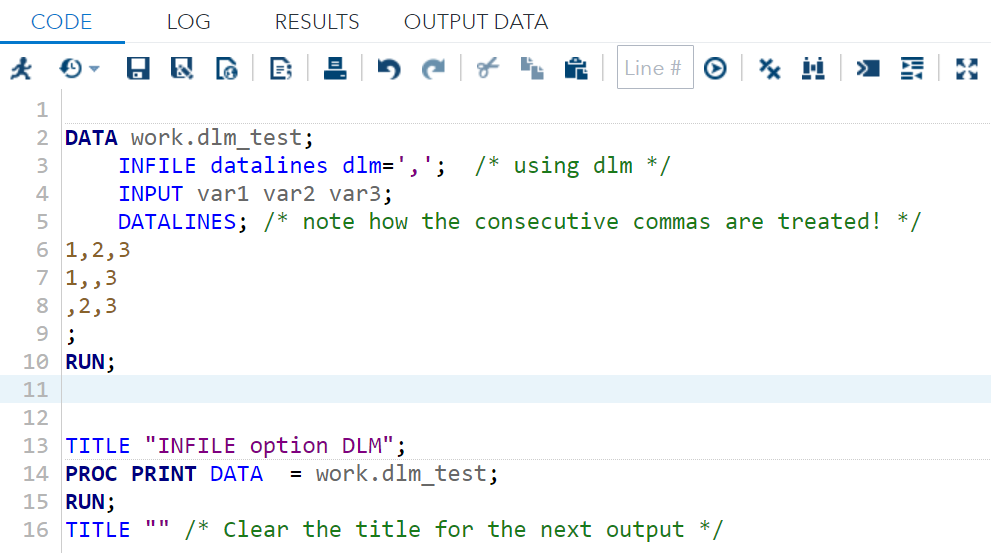
\includegraphics[width=1\linewidth]{img04/w04-INFILEoptionDLM} 

}

\caption{INFILE option: DLM.}\label{fig:unnamed-chunk-26}
\end{figure}

\begin{center}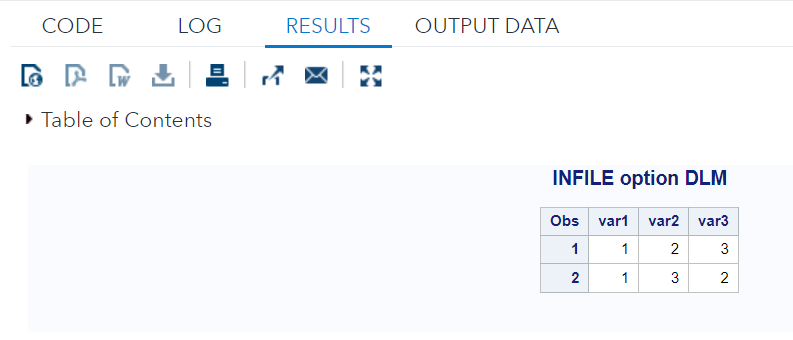
\includegraphics[width=1\linewidth]{img04/w04-DLM-output} \end{center}

Note that in the above output, only 2 observations because of the default FLOWOVER functionality (i.e., by default, the input pointer moves to the next record to fulfill the number of variables used in the input statement if some of the variables are missing in the first line.). Also, the final `3' is ignored because there is no variable to store it.

\hypertarget{dsd}{%
\subsection{\texorpdfstring{\texttt{DSD}}{DSD}}\label{dsd}}

\textbf{DSD} treats two consecutive delimiters as missing values and removes quotation marks from character values. Because of this, the following data step will read the data correctly.

\begin{figure}

{\centering 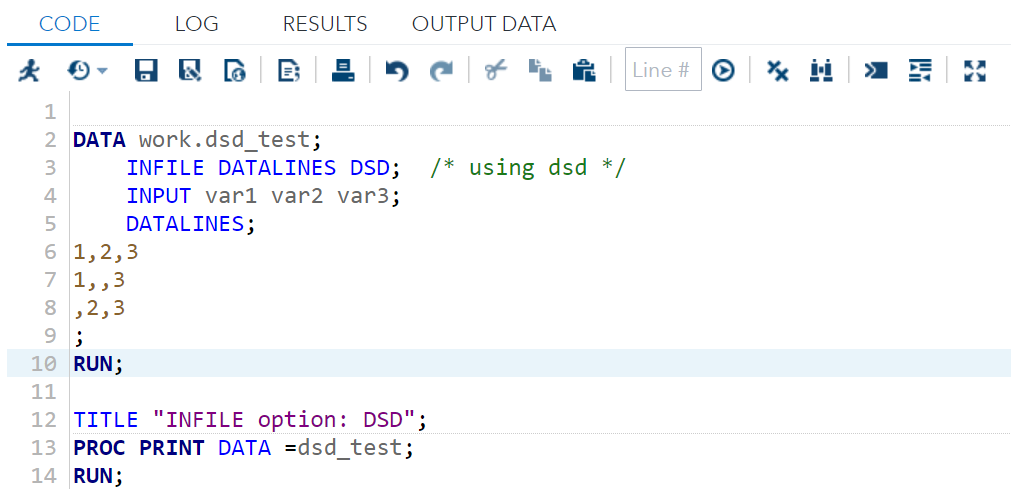
\includegraphics[width=1\linewidth]{img04/w04-InfileOptionDSD} 

}

\caption{INFILE option: DSD.}\label{fig:unnamed-chunk-28}
\end{figure}

\begin{center}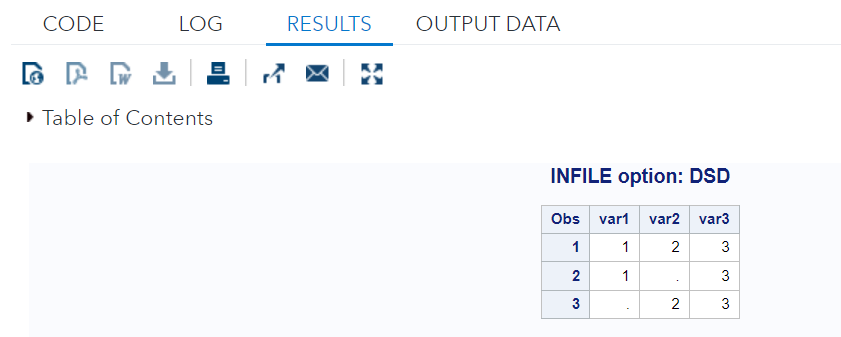
\includegraphics[width=1\linewidth]{img04/w04-dsd-output} \end{center}

\hypertarget{missover}{%
\subsection{\texorpdfstring{\texttt{MISSOVER}}{MISSOVER}}\label{missover}}

\textbf{MISSOVER} option prevents the default behavior mentioned above prevents the input pointer from moving to the next line and assigns missing values to the remaining variables. This means that if the missing values happen to be at the end of every record, the data will be read incorrectly.

\begin{figure}

{\centering 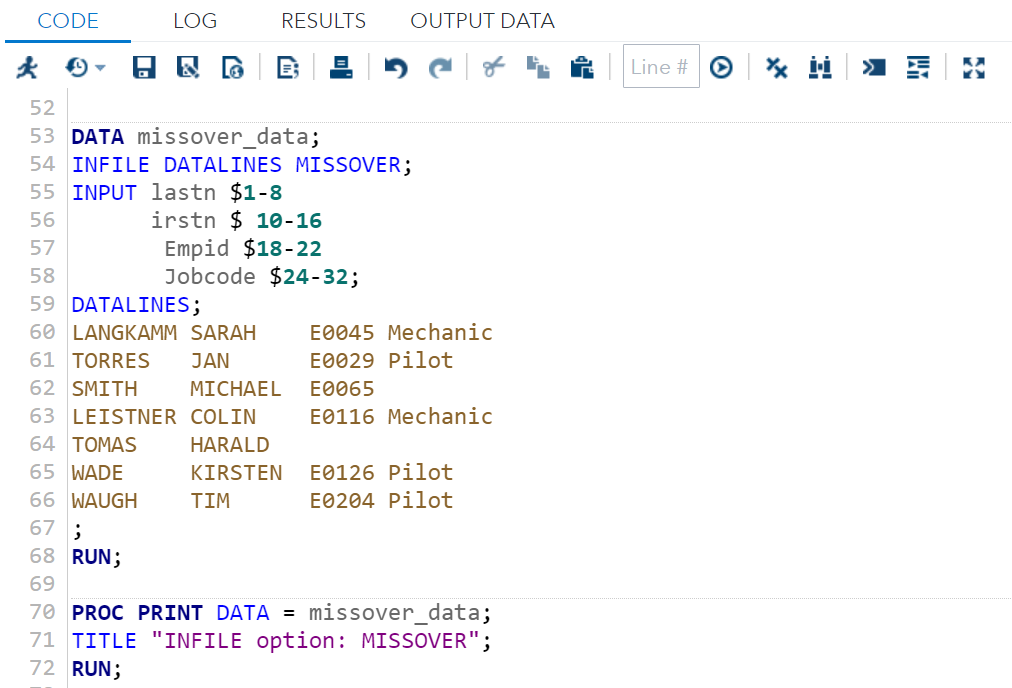
\includegraphics[width=1\linewidth]{img04/w04-InfileOptionMissover} 

}

\caption{INFILE option: MISSOVER.}\label{fig:unnamed-chunk-30}
\end{figure}

\begin{center}\includegraphics[width=1\linewidth]{img04/w04-missover-output} \end{center}

\hypertarget{reading-in-existing-sas-data-sets}{%
\section{Reading in Existing SAS Data Sets}\label{reading-in-existing-sas-data-sets}}

It is quite often to have SAS format data files. To load SAS format data files to SAS, we only need to use \texttt{SET}statement. The syntax is given below

\begin{center}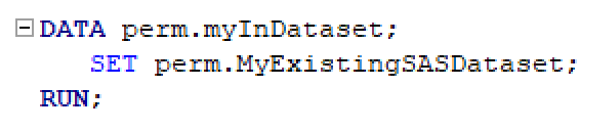
\includegraphics[width=0.7\linewidth]{img04/w04-SETstatement} \end{center}

This means we need to define a permanent library referring to the folder in which the SAS data files are stored. Note that INPUT and INFILE statements will not work since INPUT reads raw data from an external file (with INFILE statement) or from in-stream data lines (with DATALINES) in order to create SAS variables and observations.

\textbf{If two data sets with same variable names}, we can use SET statements to stack the data sets. This will be discussed in detail later in data manipulation.

\hypertarget{reading-data-via-wizard}{%
\section{Reading Data via Wizard}\label{reading-data-via-wizard}}

SAS has a data import wizard that allows users to import data from different applications. To use the import wizard in base SAS 9.4 (Windows), \texttt{Files\ -\textgreater{}\ Import\ wizard}, users can find the list of data sources that be imported to SAS without writing SAS code.

\begin{center}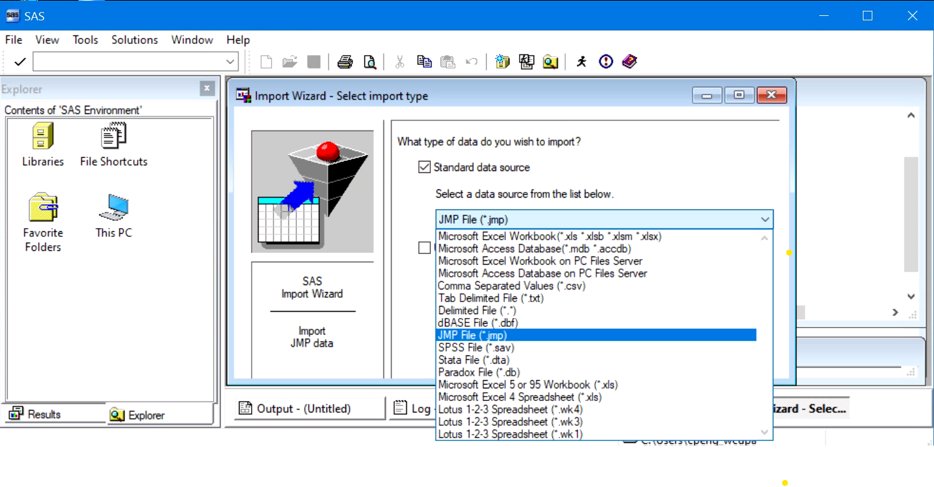
\includegraphics[width=1\linewidth]{img04/w04-importWizard} \end{center}

Then follow the self-directed steps to load data to SAS. The converted SAS data will be stored in the temporary library. The GUI of SAS studio is slightly different but has almost the same data formats.

\begin{center}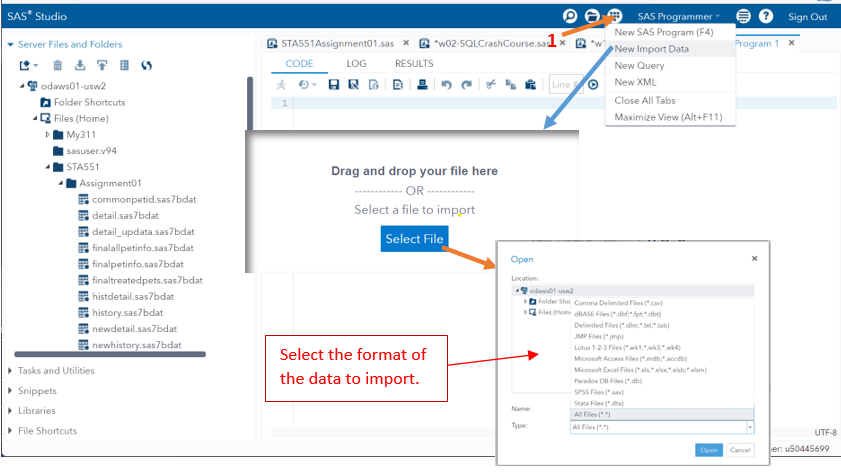
\includegraphics[width=1\linewidth]{img04/w04-SASstudioWizardGUI} \end{center}

\hypertarget{loading-data-proc-import}{%
\section{Loading Data PROC IMPORT}\label{loading-data-proc-import}}

The point-n-click approach with import wizard can load one or a few data sets. In practice, we have hundreds of data sets to load to SAS for certain projects, in this case, manual loading with Wizard will be feasible. We need to load many data sets programmatically. This is particularly important in any analytic task that involves automation that prevents human intervention from the analysis process.

PROC IMPORT will do the trick. A good feature of importing Wizard in SAS is that it generates SAS code to perform the task that the Wizard performed. To explain, we assume a delimiter data file is stored in a physical location (my SAS Studio via OnDemand):

\begin{verbatim}
Region&State&Month&Expenses&Revenue
Southern&GA&JAN2001&2000&8000
Southern&GA&FEB2001&1200&6000
Southern&FL&FEB2001&8500&11000
Northern&NY&FEB2001&3000&4000
Northern&NY&MAR2001&6000&5000
Southern&FL&MAR2001&9800&13500
Northern&MA&MAR2001&1500&1000
;
\end{verbatim}

The procedure \texttt{PROC\ IMPORT} reads the above data file with the following code

\begin{center}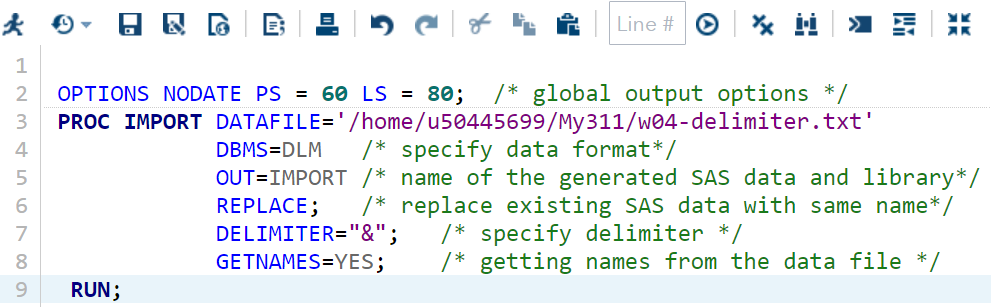
\includegraphics[width=1\linewidth]{img04/w04-ProcImport} \end{center}

SAS log will duplicate the above code and convert the PROC IMPORT to the standard DATA step code.

\begin{center}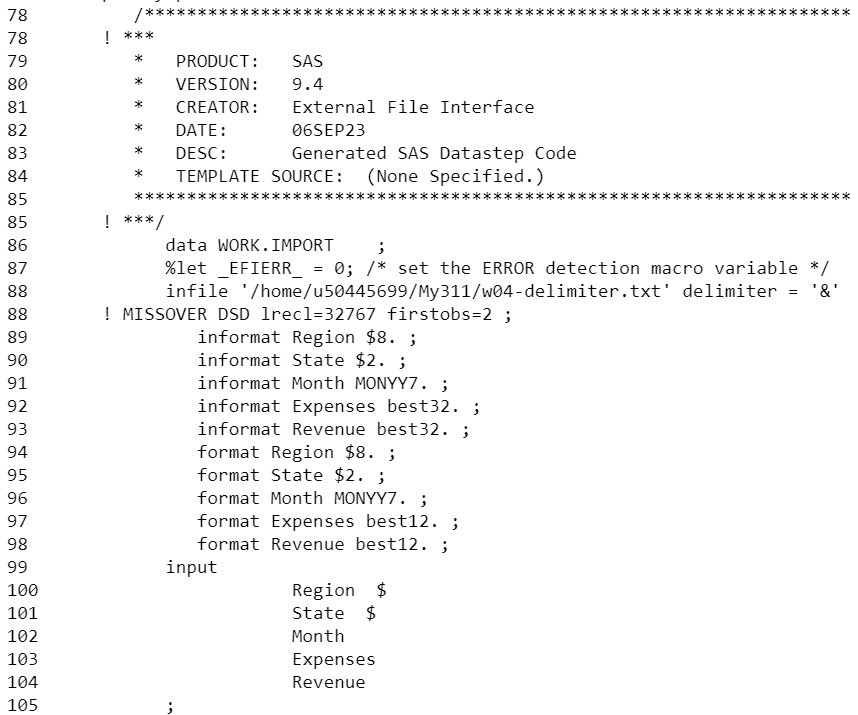
\includegraphics[width=1\linewidth]{img04/w04-ImportLog} \end{center}

The following output SAS data shows that the data loaded correctly.

\begin{center}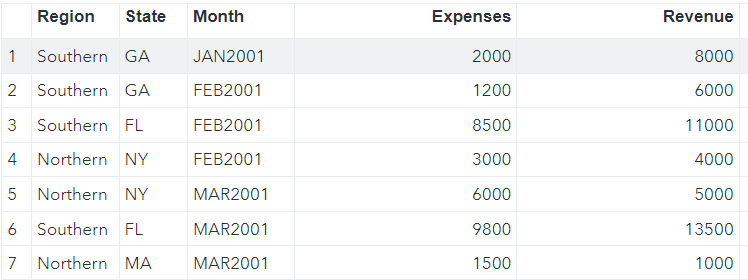
\includegraphics[width=1\linewidth]{img04/w04-PROCIMPORToutput-data} \end{center}

\hypertarget{read-data-with-url}{%
\section{Read Data with URL}\label{read-data-with-url}}

SAS can also read data from a remote computer via the internet or connect SAS to a database. The following is an example of reading a data file from the GitHub Data repository using \texttt{PROC\ IMPORT}.

\begin{center}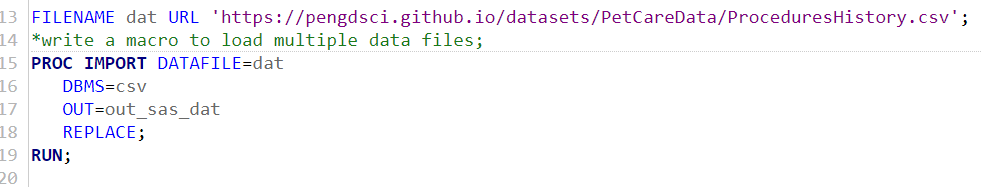
\includegraphics[width=1\linewidth]{img04/w04-readDatURL} \end{center}

\hypertarget{learning-coding-by-examples}{%
\section{Learning Coding by Examples}\label{learning-coding-by-examples}}

This section uses several examples to explain different ways of loading different formats of data files to SAS. For convenience, the working data files used in the examples were uploaded to my GitHub repository. \url{https://raw.githubusercontent.com/pengdsci/STA311/main/w04-iris-csv.csv}, \url{https://raw.githubusercontent.com/pengdsci/STA311/main/w04-iris-text.txt},
\url{https://github.com/pengdsci/STA311/raw/main/w04-iris-xls.xls}
\url{https://github.com/pengdsci/STA311/raw/main/w04-iris-xlsx.xlsx}

\begin{verbatim}
/********************************************************************
         Topics: 1. Handling challenging source data
                   (text data via INPUT or INFILE-INPUT Statements)
                 2. Read DELIMITERED data files
                 3. Read data using INPUT WIZARD
                 4. Data formats: Excel, CSV and Text
                 5. Loading the SAS dataset to SAS
                 6. EXPORT SAS data to CSV 
********************************************************************/

DM 'CLEAR LOG';
DM 'CLEAR OUT';

OPTIONS PS=90 LS=70 NOCENTER NONUMBER NODATE;

/** library on the RAMCLOUD - synchronizing files between my computer and 
    my OneDrive on the RamCloud                        **/
LIBNAME w04 "C:\STA311\w04";

/*NNNNNNNNNNNNNNNNNNNNNNNNNNNNNNNNNNNNNNNNNNNNNNNNNNNNNNNNNNNNNNNNNNNN
 Topic 1: Reading challenging data: external and in-line 
          Challenges: missing values, character variables
                      string value contains blanks, special
                      formatted numerical values, etc. 
NNNNNNNNNNNNNNNNNNNNNNNNNNNNNNNNNNNNNNNNNNNNNNNNNNNNNNNNNNNNNNNNNNNNNN*/

/* Missing values at the end of the record: MISSOVER!!
   INFILE statement's MISSOVER option to read records when
   some of the values are missing at the end of a record  */

DATA reading;                   /* temporary SAS data  */
    INFILE DATALINES  MISSOVER; /* INFILE-DATALINES read in-line data */
    INPUT Name $ Week1-Week5;   /* shortcut of patterned variable names */
    /* Caution: Records 3 and 4 have trailing missing values.  */
    DATALINES; 
Robin 3 2 5 1 6
Jack 4 4 4 3 4
Tim 3 0 0
Martin 1 0 1 1
Caroline 2 3 4 5 6
;
RUN;

PROC PRINT DATA = reading;
    TITLE 'Summer Reading Program';
    VAR Name Week1-Week5;   /* Caution: In proc print, the variable type
                            should NOT be specified. Otherwise, an error 
                               will be written to the log               */
RUN;



/* Missing values in the middle or at the end of the record: DSD!!
   INFILE statement's DSD option to read records when some of the values 
   are missing in the middle or at the beginning of a record          */

/* delimiter sensitive data - DSD */
DATA survey;
    LENGTH Name $ 9;                 /* Katherine has 9 characters!   */
    INFILE DATALINES DLM=',' DSD;  /* 1. in-line data is comma delimited
                                      2. Missing values occurred in the       
                                           middle of the records */
    INPUT Name $ (Q1-Q5) ($);     /* Pay attention to the character 
                                       variables with patterned names! */
    DATALINES;
Robert,,A,C,A,D
William,B,C,A,D,A
Linda,C,B,,A,C
Lisa,D,D,D,C,A
Katherine,A,B,C,D,A
RUN;

PROC PRINT DATA = survey;
    TITLE 'Survey Results';
    VAR Name Q1-Q5;          /* Requested character variables without the
                                specification of var type!             */
RUN;

/* The following program illustrates that the DSD option can also be used 
      i) When there is a missing value at the beginning of a record, and 
     ii) When the data are delimited by blanks (in conjunction with the DLM= option): */

DATA survey;
    LENGTH Name $ 9;             
    infile DATALINES DLM=' ' DSD;
    input Name $ (Q1-Q5) ($);
    DATALINES;
Robert  A C A D
William B C A D A
Linda C B  A C
 D D D C A
Katherine A B C D A
RUN;

PROC PRINT data = survey;
    title 'Survey Results';
    var Name Q1-Q5;
RUN;


/** Modifiers (&) and (:) - modifier list input for some challenges 
    in text data files:
1.  The ampersand (&) modifier allows you to read character values that 
contain embedded blanks.
      
   CAUTION: The ampersand (&) that follows the city variable in the INPUT 
       The statement tells SAS that the city values may contain one or more 
       SINGLE embedded blanks. Because the ampersand modifier is used, SAS 
       will read the city value UNTIL TWO OR MORE CONSECUTIVE blanks are 
       encountered. 

       That is a very important point!!!!

       When you use ampersand modified list input, the values that you are 
       reading in must be separated by two or more consecutive blanks. 
                
       You cannot use any other delimiter to indicate the end of each field.

2.  The colon (:) modifier allows you to read nonstandard data values and 
     character values that are longer than eight characters, 
     but which have no embedded blanks.
**/

DATA citypops;
   INFILE DATALINES FIRSTOBS = 2;
   INPUT city pop2000;   /* This will not be correct!  
                            (1) city is a character variable. 
                            (2) Some of its value involves embedded blank. 
                            (3) Variable length is also an issue     */
   DATALINES;
City  Yr2000Popn
New York  8008278
Los Angeles  3694820
Chicago  2896016
Houston  1953631
Philadelphia  1517550
Phoenix  1321045
San Antonio  1144646
San Diego  1223400
Dallas  1188580
San Jose  894943
;
RUN;

PROC PRINT data = citypops;
   title 'The citypops data set';
RUN;


/** The issues in the above code were fixed in the following code **/
DATA citypops;
    INFILE DATALINES FIRSTOBS = 2;
    LENGTH city $ 12;
    INPUT city & pop2000;
    DATALINES;
City  Yr2000Popn
New York  8008278
Los Angeles  3694820
Chicago  2896016
Houston  1953631
Philadelphia  1517550
Phoenix  1321045
San Antonio  1144646
San Diego  1223400
Dallas  1188580
San Jose  894943
;
RUN;

PROC PRINT data = citypops;
    TITLE 'The citypops data set: with &';
    format pop2000 comma10.;
RUN;

/******************************************************************************
  The colon (:) modifier allows us to use list input to read nonstandard data 
  values and character values that are longer than eight characters, but which 
  contain no embedded blanks. The colon (:) indicates that values are read 
  until a blank (or other delimiters) is encountered, and then an informat is 
  applied. If an informat for reading character values is specified, the w value 
  specifies the variable's length, overriding the default length of 8.       
*******************************************************************************/

DATA citypops_colon;
    INFILE DATALINES FIRSTOBS = 2;
    INPUT city & $12. pop2000 : comma.; 
    /*  & --> will take care of one or more SINGLE blanks
              in the first character variable.
        $12. -->  takes care of variable type and LENGTH, 
                  caution: (.) is required!
         : --> tells SAS to read until a blank (or other 
               delimiter) is encountered, and then an 
                informat is applied. Here, comma. is the informat. 

      Caution: Since in this example, the INFORMAT is 
                comma, so the delimiter should not be a comma!  */
DATALINES;
City  Yr2000Popn
New York  8,008,278
Los A ngeles  3,694,820
Chicago  2,896,016
Houston  1,953,631
Philadelphia  1,517,550
Phoenix  1,321,045
San Antonio  1,144,646
San Diego  1,223,400
Dallas  1,188,580
San Jose  894,943
;
RUN;

PROC PRINT DATA = citypops_colon;
    TITLE 'The citypops data set: Both (&) and (:)';
    FORMAT pop2000 comma10.;
RUN;



DATA citypops_no_colon;
    INFILE DATALINES FIRSTOBS = 2;
    INPUT city & $12. pop2000 ;
    /*  & --> will take care of one or more SINGLE blanks
             in the first character variable.
        $12. -->  takes care of variable type and LENGTH, 
                caution: (.) is required!
       : --> tells SAS to read until a blank (or other 
              delimiter) is encountered, and then an 
              informat is applied. Here, comma. is the informat. 

      Caution: Since in this example, the INFORMAT is 
               comma, so the delimiter should not be a comma! */
DATALINES;
City  Yr2000Popn
New York  8,008,278
Los A ngeles  3,694,820
Chicago  2,896,016
Houston  1,953,631
Philadelphia  1,517,550
Phoenix  1,321,045
San Antonio  1,144,646
San Diego  1,223,400
Dallas  1,188,580
San Jose  894,943
;
RUN;

PROC PRINT DATA = citypops_no_colon;
    TITLE 'The citypops data set: Both (&) and (:)';
    FORMAT pop2000 comma10.;
RUN;



/*NNNNNNNNNNNNNNNNNNNNNNNNNNNNNNNNNNNNNNNNNNNNNNNNNNNNNNNNNNNNNNNNNNNNNNNN
 Topic 3: Read external data with common formats: Excel, CSV, Text,
          and data from other applications such as SPSS using PROC IMPORT
NNNNNNNNNNNNNNNNNNNNNNNNNNNNNNNNNNNNNNNNNNNNNNNNNNNNNNNNNNNNNNNNNNNNNNNNNN*/

PROC IMPORT OUT= WORK.Iris_TEMPLATE02  /* SAS file in the temporary library  */
            DATAFILE= "C:\STA311\w04\w04-iris-xlsx.xlsx"  /* source xlsx file */
            DBMS=EXCEL REPLACE;    /*File type, replace if already exists*/
            RANGE="'w04-iris$'";   
            /*Indicates the name of the sheet within the Excel workbook
                    Note that sheet names can only be 31 characters long.  */ 
                           
            GETNAMES=YES; /*Indicates the first row contains variable names. 
                            The default setting and SAS will automatically use 
                            the first row of data as variable names.  
                                  If the first row of your sheet does not contain 
                                  variable names use the getnames=no.*/
            MIXED=YES; /*Indicates both numeric and character variables in the
                         data set. SAS uses the  first eight rows of data to 
                         determine whether the variable should be read as 
                               character or numeric.  The default setting mixed=no 
                               assumes that each variable is either all characters or 
                               all numeric. If you have a variable with both 
                               character and numeric values or a variable with missing 
                               values use mixed=yes statement to be sure SAS will 
                               read it correctly.                            */
            SCANTEXT=YES; /*Tells SAS to scan columns to determine the length of 
                            the text values*/
            USEDATE=YES;  /*Tells SAS to assign a DATE format to date data*/
            SCANTIME=YES; /* Tells SAS to assign a TIME format to time data */
RUN;

PROC PRINT;
RUN;

PROC CONTENTS DATA = Iris_TEMPLATE02;
RUN;




/**    Make sure SAS can find the CSV data file    **/
PROC IMPORT DATAFILE = "C:\STA311\w04\w04-iris-csv.csv" 
    OUT = IRISCSV       /* name of the SAS data set to send to the 
                           temporary library  */
    DBMS = CSV          /* Database management system: CSV */
    GETNAMES = YES;   /* The first row is not a record. */
 ;
RUN;

PROC IMPORT DATAFILE = "C:\STA311\w04\w04-iris-text.txt" 
    OUT = TEXTIRIS         /*  */
    DBMS = CSV  REPLACE;
    GETNAMES = YES;
RUN;


PROC IMPORT OUT= WORK.demographics 
            DATAFILE= "C:\STA311\w04\w04-Demographics.sav" 
            DBMS=SPSS REPLACE;
RUN;



/*NNNNNNNNNNNNNNNNNNNNNNNNNNNNNNNNNNNNNNNNNNNNNNNNNNNNNNNNNNNNNNNNNNNNNNN
 Topic 4:  Export SAS data set to a CSV format data
           Why CSV?
           The CSV (short for "comma-separated values") is one of the most
           flexible formats. CSV is a bit faster, smaller in size, and very easy 
           to handle (even in Excel) and many existing applications understand 
           it, it is a widely used standard. It is still the first choice in 
           many situations.

          This is why I only use an example to demonstrate this programmatic
          approach to export CSV data!
NNNNNNNNNNNNNNNNNNNNNNNNNNNNNNNNNNNNNNNNNNNNNNNNNNNNNNNNNNNNNNNNNNNNNNNNNNNN*/

PROC EXPORT DATA= IRIS_template   /* Export the SAS file from the permanent 
                                     library and save it as a CSV file in the 
                                     next folder. */
            OUTFILE= "C:\STA311\w04\outcsv_mycsv.csv" 
            DBMS=CSV REPLACE;  /* REPLACE will overwrite the existing csv file 
                                  with the same name. */
     PUTNAMES=YES;     /* carry names of the variables in the SAS data file */
RUN;

/**    Why do we need PROC IMPORT/EXPORT while we have INPUT WIZARD?    **/

/*NNNNNNNNNNNNNNNNNNNNNNNNNNNNNNNNNNNNNNNNNNNNNNNNNNNNNNNNNNNNNNNNNNNNNNNNNNNNNN
 Topic 5:  Loading SAS Data set to SAS for DATA MANAGEMENT
           We only focus on the syntax and some basic controls this time.
           We will use this SET statement frequently beyond this point.
  
           Basic Syntax:

           DATA newdata;
           SET oldSASdataset;
             more statements to modify the oldSASdataset;
           RUN;
           
NNNNNNNNNNNNNNNNNNNNNNNNNNNNNNNNNNNNNNNNNNNNNNNNNNNNNNNNNNNNNNNNNNNNNNNNNNNNN*/

    /****  A simple example: Citypops.sas7bdat is in the temporary library ***/

  PROC PRINT DATA = Citypops;
  TITLE "Old City Population Data Set";
  RUN;

  DATA NewCityPops;
  SET CityPops;
      New_popn = ROUND(pop2000 * 1.0001, 1); /* add a new variable reflecting
                                                the new population size. 
                                               */
  RUN;

  /**   ROUND() is an SAS built-in function: The following examples illustrate 
                how to use it:
                       round(1234.56789, 100)-----> 1200; 
                       round(1234.56789, 10) -----> 1230; 
                       round(1234.56789, 1)  -----> 1235; 
                       round(1234.56789, .1) -----> 1234.6;
                       round(1234.56789, .01)-----> 1234.57; 
                       round(1234.56789, .001)----> 1234.568;  
                       round(1234.56789, .0001)---> 1234.5679; 
                       round(1234.56789, .00001)--> 1234.56789;
                       round(1234.56789, .1111)---> 1234.5432;        **/

PROC PRINT DATA = NewCityPops;
TITLE "New City Population Data";
RUN;

TITLE " ";  /* clear the title for next output  */
\end{verbatim}

\hypertarget{descriptive-statistics}{%
\chapter{Descriptive Statistics}\label{descriptive-statistics}}

Once we finish reading data to SAS, we can use SAS to perform basic descriptive analysis such as frequency tables, different charts for numerical measures, etc. For convenience, we use the following data set for all illustrative examples in this chapter.

This is data about penguins collected by Dr.~Kristen Gorman and the Palmer Station in Antarctica. There are 344 cases and 7 columns. With both numerical and categorical variables, there are options for exploring, including looking for differentiators between the three species of penguin.

\url{https://raw.githubusercontent.com/pengdsci/sta553/main/w02-penguins.csv}

\begin{verbatim}
FILENAME pguin URL "https://raw.githubusercontent.com/pengdsci/sta553/main/w02-penguins.csv";

PROC IMPORT DATAFILE = pguin
    OUT = penguin        
    DBMS = CSV  
    REPLACE;
    GETNAMES = YES;
RUN;
\end{verbatim}

We first look at the types of variables in the working data set using \texttt{PROC\ CONTENTS}.

\begin{verbatim}
TITLE "Information of Penguin Data";
PROC CONTENTS DATA = penguin;
RUN;
\end{verbatim}

The output contains three tables, the second table contains information about the SAS engine. We only look at the first and the third table that contains data information.

\begin{center}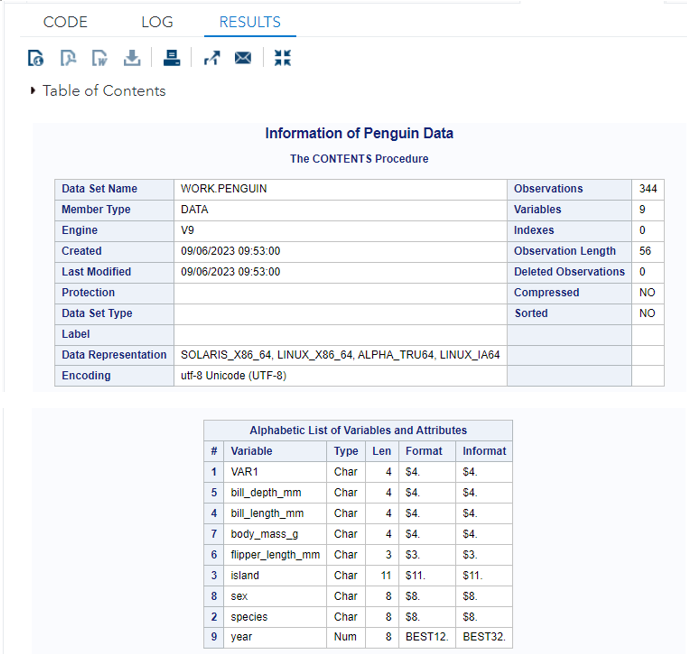
\includegraphics[width=1\linewidth]{img05/w05-DataContents} \end{center}

We can see that there are 344 observations and 9 variables. All variables in the data set are in numerical form except for the year. We will use a SAS function to convert character variables to numerical variables in order to do appropriate analyses.

\hypertarget{frequency-table-analysis}{%
\section{Frequency Table Analysis}\label{frequency-table-analysis}}

We can use \texttt{PROC\ FREQ} to produce frequency tables based on categorical variables. We can also group numerical variables to create categorical variables and then create frequency tables. Group variables in a data set are considered as data manipulation, We will discuss this in later chapters. The next examples will use the existing categorical variables in the data set.

\begin{verbatim}
TITLE "Frequency by species and locations";
PROC FREQ DATA=penguin;
  TABLES species;  /* species table */
  TABLES island;   /* location table */
RUN;
\end{verbatim}

The above two procedures give the frequency distributions of \texttt{species} and \texttt{island} in the same procedure. A SAS program consists of individual data and procedure steps. Each procedure allows only one title and a few sub-titles, all titles and sub-titles are always printed on the top of the output of the procedure.

\begin{center}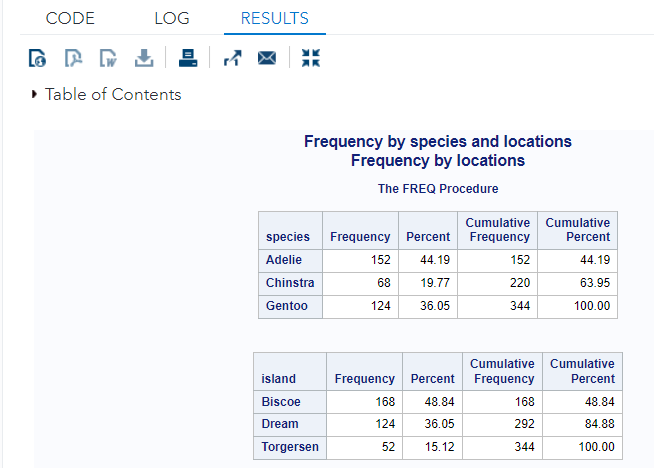
\includegraphics[width=1\linewidth]{img05/w05-1wayFreqTable} \end{center}

We can use two procedure steps to give specific titles for individual tables. We may want to know whether a particular species of penguin likes to live in a particular location. The two-way frequency table (cross-tabulation) gives this type of information.

\begin{verbatim}
TITLE "Two-way Frequency Table";
PROC FREQ DATA=penguin;
  TABLES species * island;  /* species table */
RUN;
\end{verbatim}

\begin{center}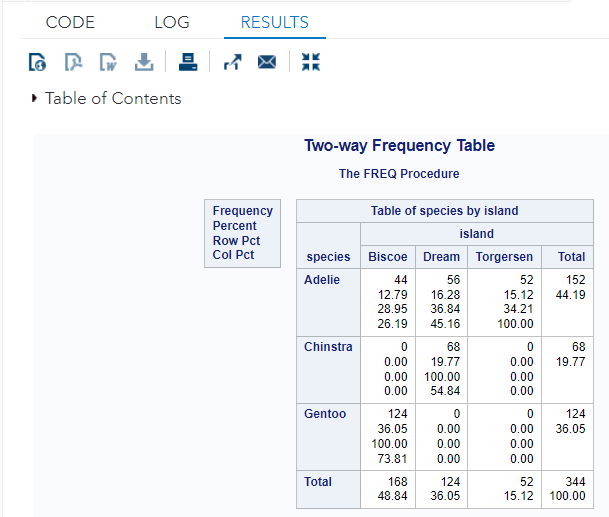
\includegraphics[width=1\linewidth]{img05/w05-2wayFreqTable} \end{center}

Note the asterisk (*) between the variables \texttt{species} and \texttt{island} on the tables statement. The above two-way table contains four different frequencies. Sometimes, we may be interested in only one type of frequency. We can select a particular frequency to print out by using the \texttt{norow}, \texttt{nocol}, and \texttt{nofreq} options on the tables statement to suppress the printing of the row percentages, column percentages, and frequencies (leaving just the cell percentages). Note that the options come after the forward-slash ( / ) on the tables statement.

\begin{verbatim}
TITLE "Two-way Relative Frequency Table";
PROC FREQ DATA=penguin;
  TABLES species * island / NOROW NOCOL NOFREQ ;
RUN;
\end{verbatim}

Note that the order of the options does not matter.

\begin{center}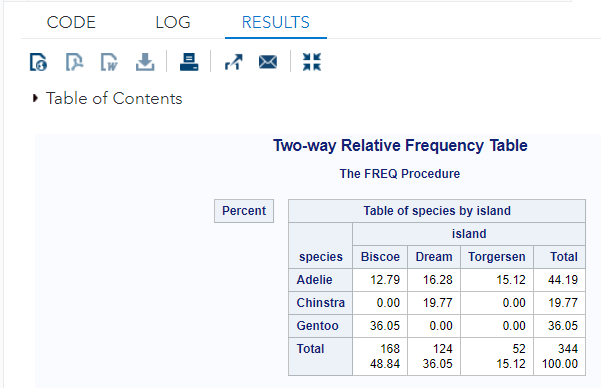
\includegraphics[width=1\linewidth]{img05/w05-2wayFreqRelTable} \end{center}

\hypertarget{numerical-summary-statistics}{%
\section{Numerical Summary Statistics}\label{numerical-summary-statistics}}

In elementary statistics, we learned several numerical measures of numerical data (variable) SAS procedures \texttt{PROC\ MEANS} and \texttt{PROC\ UNIVARIATE} calculate these numerical summary measures and also create plots such as basic statistical graphics as by-products.

Since some of the numerical variables stored in the data are in the character form, we first convert them back to numerical form in order to perform appropriate analysis.

\begin{verbatim}
DATA new_penguin;  /* define a new data set */
   SET Penguin;    /* copy the data original data*/
   body_mass = input(body_mass_g, 8.);  /* conversion */
   flipper_length = input(flipper_length_mm, 8.);
   bill_depth = input(bill_depth_mm, 8.);
   bill_length = input(bill_length_mm, 8.);
RUN;

PROC CONTENTS DATA  = new_penguin; /* check the conversion */
RUN;
\end{verbatim}

\begin{center}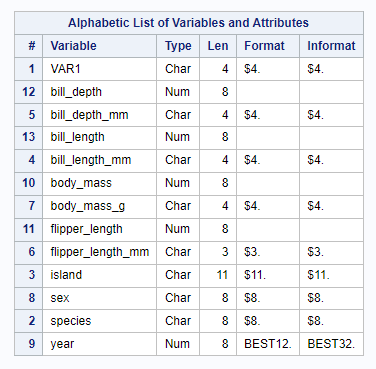
\includegraphics[width=0.7\linewidth]{img05/w05-ConvertedDataSet} \end{center}

\hypertarget{proc-means}{%
\subsection{\texorpdfstring{\texttt{PROC\ MEANS}}{PROC MEANS}}\label{proc-means}}

\texttt{PROC\ MEANS} calculates the summarized statistics such as means, quartiles, size, etc. The detailed list of options is given in the following table.

\begin{center}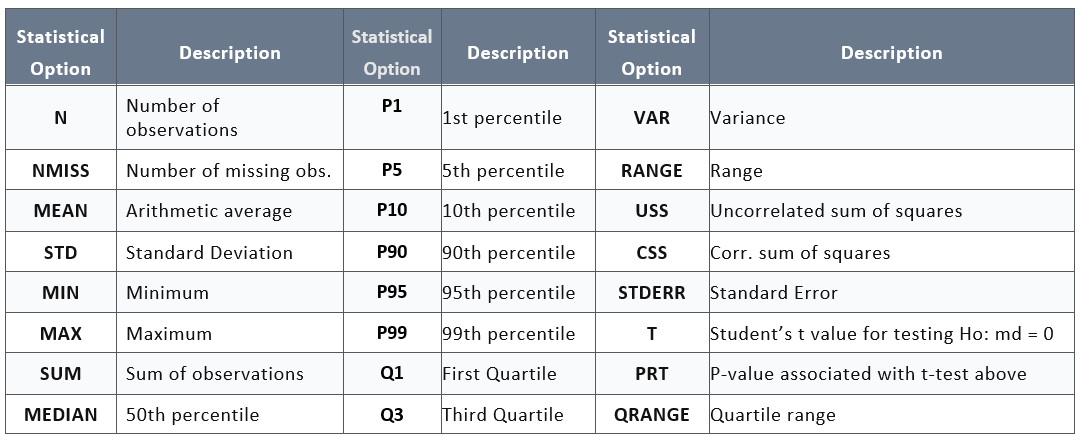
\includegraphics[width=1\linewidth]{img05/w05-ProcMeansOptions} \end{center}

In the following example, we selected several summary statistics to report in \texttt{PROC\ MEANS}.

\begin{verbatim}
TITLE "Summary Statistics by PROC MEANS";
PROC MEANS DATA=new_penguin N MIN Q1 MEAN STD MEDIAN Q3 MAX;
  VAR body_mass;
RUN;
\end{verbatim}

\begin{center}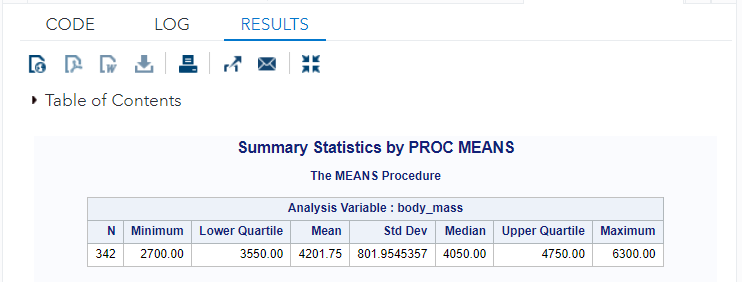
\includegraphics[width=1\linewidth]{img05/w05-ProcMeansTables} \end{center}

Suppose we would like to get the summary statistics separately for different species. We can use the class statement (shown below) to get separate results for the different values of \texttt{species}.

\begin{verbatim}
TITLE "Summary Statistics by SPECIES";
PROC MEANS DATA=new_penguin N MIN Q1 MEAN STD MEDIAN Q3 MAX;
  CLASS species;
  VAR body_mass;
RUN;
\end{verbatim}

\begin{center}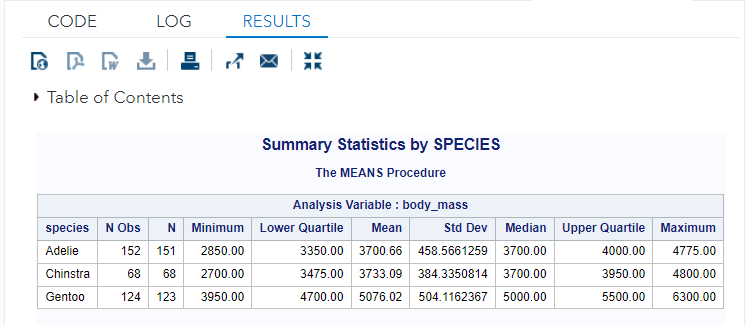
\includegraphics[width=1\linewidth]{img05/w05-ProcMeansTablesBySpecies} \end{center}

We can also save the output of the summary table as a SAS data set.

\begin{verbatim}
  
TITLE "Summary Statistics by OUTPUT SAS dataset";
PROC MEANS DATA=new_penguin N MIN Q1 MEAN STD MEDIAN Q3 MAX;
  CLASS species;
  VAR body_mass;
  OUTPUT OUT= SummaryPenguin /autoname;
RUN; 
  
PROC PRINT;
RUN;
\end{verbatim}

\begin{center}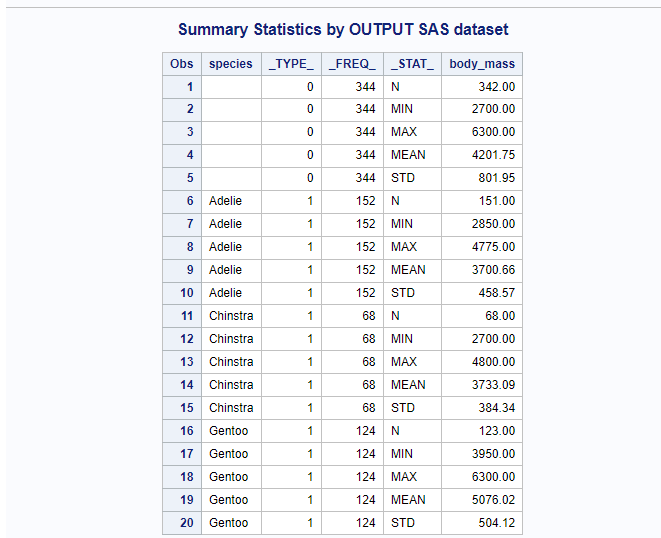
\includegraphics[width=1\linewidth]{img05/w05-outputSummaryData} \end{center}

\hypertarget{proc-univariate}{%
\subsection{\texorpdfstring{\texttt{PROC\ UNIVARIATE}}{PROC UNIVARIATE}}\label{proc-univariate}}

We first look at the univariate analysis using \texttt{PROC\ UNIVARIATE}.

\begin{verbatim}
PROC UNIVARIATE DATA=new_penguin;
  VAR body_mass;
RUN;
\end{verbatim}

The output tables of \texttt{PROC\ UNIVARIATE} are summarized in the following.

\begin{center}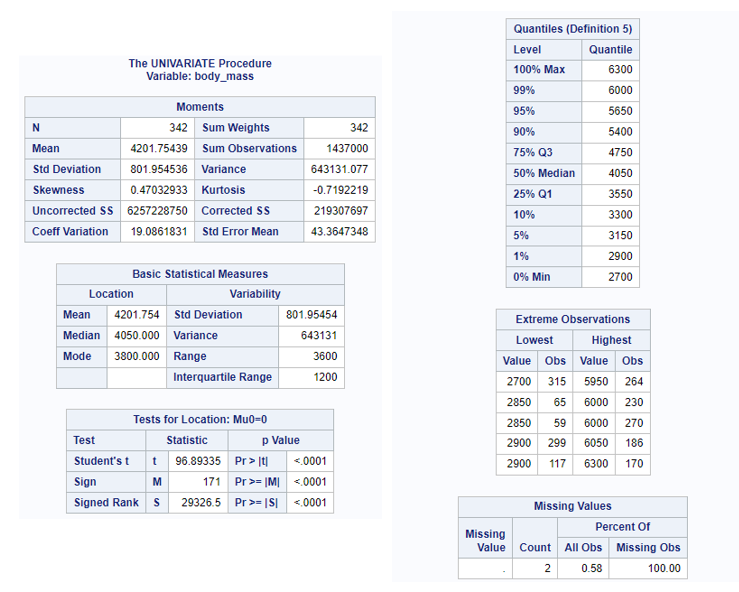
\includegraphics[width=1\linewidth]{img05/w05-UnivariateOutput} \end{center}

\hypertarget{learning-coding-by-examples-1}{%
\section{Learning Coding by Examples}\label{learning-coding-by-examples-1}}

The following examples contain more detailed information on the three procedures: MEANS, FREQ, and UNIVARIATE.

We still use the iris data set in different formats that can be found at

\url{https://raw.githubusercontent.com/pengdsci/STA311/main/w04-iris-csv.csv}, \url{https://raw.githubusercontent.com/pengdsci/STA311/main/w04-iris-text.txt},
\url{https://github.com/pengdsci/STA311/raw/main/w04-iris-xls.xls}
\url{https://github.com/pengdsci/STA311/raw/main/w04-iris-xlsx.xlsx}

Some inferential information introduced in various examples is not required for this class. We keep this type of information in this note to make the ePack a useful reference book.

\begin{verbatim}
/**********************************************************
    Author: Cheng Peng
      Date: 2/15/2021
 Topics  1. Loading tab and csv file to SAS
         2. PROC MEANS Basics
         3. PROC MEANS - beyond averages
         4. PROC FREQ Basics
         5. PROC UNIVARIATE basics
***********************************************************/
DM "CLEAR LOG";
DM "CLEAR OUT";

LIBNAME w05 "C:\STA311\w05";
OPTIONS PS = 94 LS =74 NODATE NONUMBER NOCENTER;



/*******************************************************
      Topic 1: Loading Data with Data and PROC step

      Read text and csv data into SAS with DATA STEP
      and PROC IMPORT - Pay attention to the DELIMITER
      When using INFILE-INPUT statement in a data step
********************************************************/

/** txt - tab-delimited data **/
DATA TXTIRIS;
LENGTH variety $ 10;
/* txt files are tab-delimited data. The delimiter of this data is '09'x
   that has to be specified in the following INFILE statement            */
INFILE "C:\STA311\w05\w05-iris-text.txt" 
        delimiter = '09'x  FIRSTOBS = 2;
INPUT SepalLengt SepalWidth  PetalLength  PedalWidth  variety $;
RUN;

PROC CONTENTS DATA = TXTIRIS;
RUN;

/** CSV - comma separated values, dlm ="," should be specified in the
    INFILE statement.                                             **/
DATA CSVIRIS;
LENGTH variety $ 10;
INFILE "C:\STA311\w05\w05-iris-csv.csv" 
          dlm="," FIRSTOBS = 2;
INPUT SepalLength SepalWidth PetalLength PedalWidth variety $;
RUN;

PROC CONTENTS DATA = CSVIRIS;
RUN;

/** PROC IMPORT Methods **/
/** PROC IMPORT TXT **/
PROC IMPORT OUT= WORK.txt_iris 
            DATAFILE= "C:\STA311\w05\w05-iris-text.txt" 
            DBMS=TAB REPLACE;   /* .txt is a tab-delimited data  */
     GETNAMES=YES;
     DATAROW=2;         /** data record starts from row 2, 
                            The first row lists variable names  **/
     GUESSINGROWS =150;  /** This option is required since the 
                            length of variety is more than 8 bytes **/
RUN;

/* PROC IMPORT - CSV */
PROC IMPORT OUT= WORK.iris_csv 
            DATAFILE= "C:\STA311\w05\w05-iris-csv.csv" 
            DBMS=CSV REPLACE;  /* database management system identifier: CSV */
     GETNAMES=YES;
     DATAROW=2;  /*  */
     GUESSINGROWS =MAX; /* Need to be specified whenever the data set has character 
                          variables. The maximum number of row SAS can guess is 
                          32767. */
RUN;


/****************************************************************
                   Topic 2. PROC MEANS
 Certain SAS procedures can only be performed on numeric data. 
 Two such procedures - PROC MEANS and PROC UNIVARIATE - are 
 illustrated here using the height/weight SAS data set. 
 (Note that PROC SUMMARY generates output similar to PROC MEANS.)

  Several Statements to know:
  1. CLASS
  2. BY
  3. OUTPUT
****************************************************************/
DM "CLEAR LOG";
DM "CLEAR OUT";

/** Example 2.1: default descriptive statistics -  
               N Mean Std Dev Minimum Maximum     **/
PROC MEANS DATA = iris_csv;    /* Begin the PROC step */
  /* Add 2 titles */
  TITLE1 'PROC MEANS:  Example 2.1';
  TITLE2 'No keywords specified';
RUN;             /* End the PROC step */

/** Explore the information in the data set **/
PROC CONTENTS DATA = IRIS_CSV;
RUN;


/******************************************************************
   Example 2.2: available keywords - all descriptive statistics 

   When using PROC MEANS, the CLASS statement avoids having
   to sort the data first, but the CLASS statement is more 
   suited to smaller data sets or when just a few CLASS 
   variables are to be used.                    
 
 Some of the keywords available with PROC MEANS:
        N - number of observations
        MEAN - mean value
        MIN - minimum value
        Q1 - first quartile
        Median - middle value of the sorted data set
        Q3 - third quartile
        MAX - maximum value
        SUM - the total values
        NMISS - number of missing values
        MAXDEC = n - setting the maximum number of decimal places 

*******************************************************************/

PROC MEANS DATA = IRIS_CSV N MIN Q1 MEDIAN MEAN Q3 MAX SUM NMISS ; 
     VAR sepal_length;
     /*Separate the analysis by values of variety */
     CLASS variety; /* CLASS statement produces a single table */

     /* Add 3 titles */
     TITLE1 'PROC MEANS:  Example 2.2';
     TITLE2 'Use of VAR, CLASS, and TITLE statements';
     TITLE3 'CLASSED by variety';
RUN;        

/* Example 2.3: BY- statement to replace CLASS statement!
                BY statement will be used frequently in the future.
                In order to use the BY statement, the data set has to
                be sorted by the CLASS variable - variety!      */
PROC SORT DATA = IRIS_CSV; 
BY variety;
RUN;

OPTION LS=150;

/* pay attention to the  */
PROC MEANS N MIN Q1 MEAN MEDIAN Q3 MAX STD SUM NMISS MAXDEC = 1 
     DATA = iris_csv MAXDEC = 3; 
     /*Separate the analysis by values of variety */
     BY variety;   /* BY statement produces three separate tables! */
     /*Apply analysis only to "sepal_length" variable*/
     VAR sepal_length;    
     /* Add 3 titles */
     TITLE1 'PROC MEANS:  Example 2.3';
     TITLE2 'Use of VAR, BY, and TITLE statements';
     TITLE3 'CLASSED by variety';
     TITLE4 "BY Statement - Produces 3 Tables";
RUN;        

/** Other descriptive statistics with PROC MEANS:

    SUM Sum of observations
    MEDIAN  50th percentile
    P1  -> 1st percentile
    P5  -> 5th percentile
    P10 -> 10th percentile
    P90 -> 90th percentile
    P95 -> 95th percentile
    P99 -> 99th percentile
    Q1  -> First Quartile
    Q3  -> Third Quartile
    *****
    VAR -> Variance
    RANGE   -> Range
    USS -> Uncorr. sum of squares
    CSS -> Corr. sum of squares
    STDERR  -> Standard Error
    T   -> Student抯 t value for testing Ho: md = 0
    PRT -> P-value associated with t-test above
    SUMWGT  -> Sum of the WEIGHT variable values
    QRANGE  -> Quartile range
    *****
    CLM -> confidence limits on the mean
    LCLM -> lower confidence limit on the mean (one-sided)
    UCLM -> upper confidence limit on the mean (one-sided)
**/

/** Example 2.4: confidence interval for mean sepal_length and 
                 sepal_width by variety                    **/

PROC MEANS DATA = IRIS_CSV   MAXDEC = 3
                 N             /* sample size */
                 MEAN          /* sample mean */
                 MAXDEC = 1    /* decimal places to keep */
                 ALPHA = 0.01  /* significant level  */
                 CLM           /* two-sided confidence limits: 99%  */
                 LCLM          /* lower confidence limit: 99% */
                 UCLM          /* upper confidence limit: 99% */
                 ; 
     /*Separate the analysis by values of variety */
     CLASS variety;   /* want to create a single table */
     /*Apply analysis only to "sepal_length" and "sepal_width" variables*/
     VAR sepal_length sepal_length; 
     /* Add 3 titles */
     TITLE1 'PROC MEANS:  Example 2.4';
     TITLE2 'Confidence Intervals: 99%';
     TITLE3 'CLASSED by variety';
RUN;        

PROC PRINT; RUN;


OPTIONS PS = 90 LS =70 NONUMBER NODATE;   /* global options */

/* Example 2.5: OUTPUT- statement creates an SAS data set that stores
                the output information from PROC MEANS! - This is another
                method for creating SAS data sets.                  */

PROC MEANS DATA = IRIS_CSV ALPHA=0.01 NOPRINT; /* Setting up confidence level.
                                 If not specified, default level 0.05  */
                 *CLM             /* suppress the output statistics */
                 N                /* sample size */
                 MEAN            /* sample mean */
                 MAXDEC = 1      /* decimal places to keep */
                 ALPHA = 0.01    /* significant level  */
                 CLM             /* two-sided confidence limits: 99%  */
                 LCLM            /* lower confidence limit: 99% */
                 UCLM            /* upper confidence limit: 99% */
                 ; 
     /*Separate the analysis by values of variety */
     CLASS variety;   /* want to create a single table */
     /*Apply analysis only to "sepal_length" and "sepal_width" variables*/
     VAR sepal_length sepal_length; 
     /* output a SAS data set */ 
     OUTPUT OUT = My_CLM            /* output SAS data set --> temp lib*/
               N = size             /* sample size */
               MEAN = avg         
               STDERR = sd_err      /* standard error */
               LCLM = LCI           /* lower confidence limit  */
               UCLM = UCI;          /* upper confidence limit  */
     /* Add 3 titles */
     TITLE1 'PROC MEANS:  Example 2.5';
     TITLE2 'Confidence Intervals: 99%';
     TITLE3 'CLASSED by variety';
RUN;        

TITLE "";  /* this clears all previous titles */

PROC PRINT; RUN;

/**************************************************************
            Topic 3:  PROC FREQ

Frequency tables and crosstabulation tables provide a way to
summarize data for ordinal and categorical variables. 
Frequency tables show the distribution of a variable's values.
**************************************************************/

/**  Example 3.1. Simple frequency table **/
PROC FREQ DATA = IRIS_CSV;
TABLE VARIETY;
TITLE "Frequency Table of Variety";
RUN;

/** Example 3.2. Output frequency table to a SAS data set 
    Frequencies and percentages calculated using Proc Freq 
    can also be saved to an output dataset using the OUT option 
    combined with the TABLES statement.
   
    The OUTCUM option can also be added to include the 
    cumulative frequencies in the output dataset          **/

PROC FREQ DATA = IRIS_CSV;
TABLE VARIETY / OUT = Variety_FREQ OUTCUM;
TITLE1 "Frequency Table of Variety";
TITLE2 "Store the output to a SAS data set";
RUN;

PROC PRINT;
TITLE "Print out the output Frequency table";
RUN;

TITLE "";

/** We will revisit PROC FREQ after we do some data manipulation **/

/**************************************************************
            Topic 4:  PROC UNIVARIATE

PROC UNIVARIATE produces descriptive statistics on continuous 
variables just like proc means, but many more of them, and also 
can produce some univariate plots.

**************************************************************/

OPTION NOCENTER LS = 90;

/* Example 4.1:  Univariate analysis of a numerical variable
                 -- a simple example                     */
PROC UNIVARIATE DATA = IRIS_CSV 
    NORMAL  /* normality test */
    FREQ    /* frequency table of sepal_length: not useful*/
    PLOT;   /* plot of the histogram of sepal_length */
    VAR Sepal_length;
    /* specification of details in the histogram
       1. Place a normal curve on the top of the histogram
    */
    HISTOGRAM Sepal_length/NORMAL;
    TITLE 'PROC UNIVARIATE EXAMPLE';
    FOOTNOTE 'Evaluate the distribution of Sepal_length';
RUN;

TITLE "";
FOOTNOTE "";


/* Example 4.2:  PROC UNIVARIATE -- OUTPUT SAS Data set     
   This is a very simple example with a few descriptive statistics  */
PROC UNIVARIATE  DATA = IRIS_CSV NOPRINT;
    VAR Sepal_length;
      OUTPUT OUT = UNIVAR_OUT_AVG          /* output data set #1 */
              MEAN = Sepal_length_avg;
    OUTPUT    OUT = UNIV_OUT_MORE        /* output data set #2 */
              /* Three descriptive statistics were written to the SAS data set */
              MEAN =Sepal_L_AVG        
              STD = Sepal_L_STD
              MIN = Sepal_L_MIN;
RUN;


/******************************************************
  Available Statistics for OUT in PROC UNIVARIATE

*** Descriptive Statistics ***
CSS ==> Sum of squares corrected for the mean
CV ==> Percent coefficient of variation
KURTOSIS | KURT ==> Measurement of the heaviness of tails
MAX ==> Largest (maximum) value
MEAN ==> Arithmetic mean
MIN ==> Smallest (minimum) value
MODE ==> Most frequent value (if not unique, the smallest mode)
N==> Number of observations on which calculations are based
NMISS==> Number of missing observations
NOBS==> Total number of observations
RANGE==> Difference between the maximum and minimum values
SKEWNESS | SKEW==> Measurement of the tendency of the deviations to be larger 
    in one direction than in the other
STD | STDDEV==> Standard deviation
STDMEAN | STDERR==> Standard error of the mean
SUM==> Sum
SUMWGT==> Sum of the weights
USS==> Uncorrected sum of squares
VAR==> Variance

**** Quantile Statistics  ****
MEDIAN | Q2 | P50==> middle value (50th percentile)
P1==> 1st percentile
P5==> 5th percentile
P10==> 10th percentile
P90==> 90th percentile
P95==> 95th percentile
P99==> 99th percentile
Q1 | P25==> Lower quartile (25th percentile)
Q3 | P75==> Upper quartile (75th percentile)
QRANGE==> Difference between the upper and lower quartiles 
           (also known as the inner quartile range)

*** Robust Statistics ***
GINI==> Gini抯 mean difference
MAD==> Median absolute difference
QN==> 2nd variation of median absolute difference
SN==> 1st variation of median absolute difference
STD_GINI==> Standard deviation for Gini抯 mean difference
STD_MAD==> Standard deviation for median absolute difference
STD_QN==> Standard deviation for the second variation of 
          The median absolute difference
STD_QRANGE==> Estimate of the standard deviation, based on 
              interquartile range
STD_SN==> Standard deviation for the first variation of the 
          median absolute difference

*** Hypothesis Test Statistics ***
MSIGN==> Sign statistic
NORMAL==> Test statistic for normality. If the sample size is less than or 
          equal to 2000, this is the Shapiro-Wilk W statistic. Otherwise, 
          it is the Kolmogorov D statistic.
PROBM==> Probability of a greater absolute value for the sign statistic
PROBN==> Probability that the data came from a normal distribution
PROBS==> Probability of a greater absolute value for the signed-rank statistic
PROBT==> Two-tailed p-value for Student抯 t statistic with  degrees of freedom
SIGNRANK==> Signed rank statistic
T==> Student t statistic to test the null hypothesis that the
     The population mean is equal to mu_0 

****************************************************/
\end{verbatim}

\hypertarget{basic-statistics-graphics}{%
\chapter{Basic Statistics Graphics}\label{basic-statistics-graphics}}

Making high-quality statistical graphics is not an easy task in early versions of SAS. Since SAS 9.2, `ODS graphics ' was introduced and supported by several SAS products (see the following list).

\begin{center}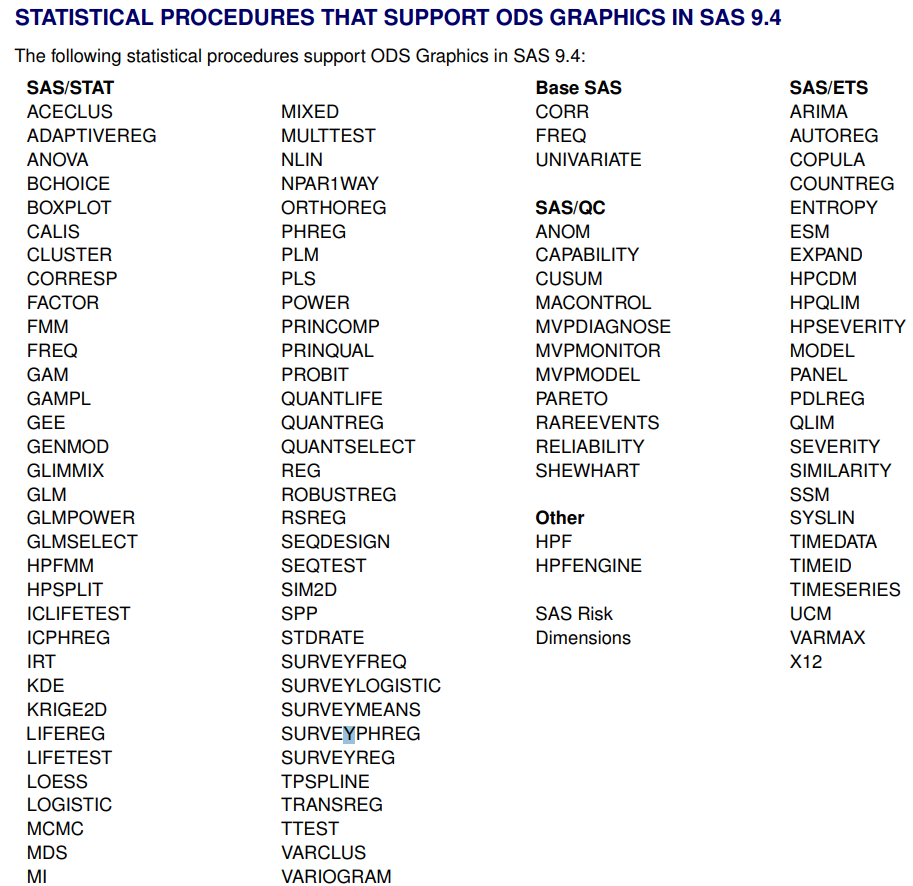
\includegraphics[width=0.8\linewidth]{img06/w06-OdsGraphicSupportedSASProducts} \end{center}

The current SAS license at WCU has a few SAS products and all of them support ODS graphics.

\begin{center}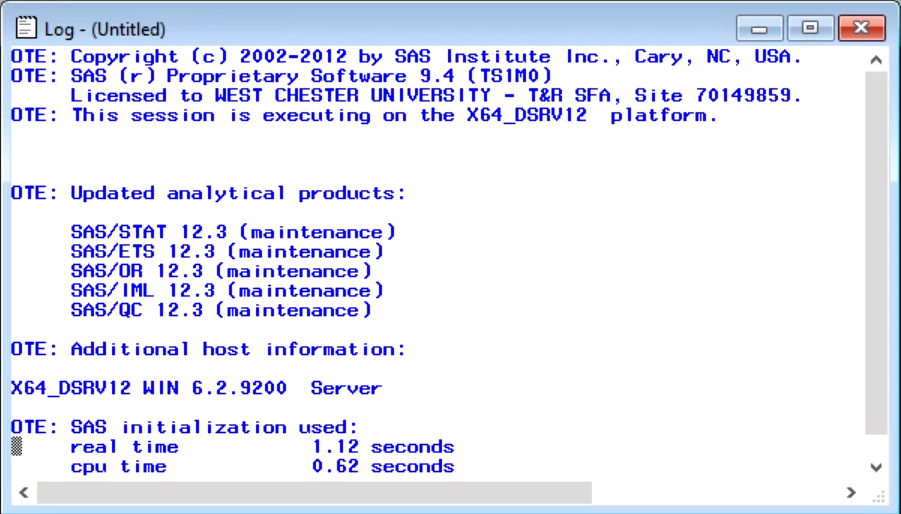
\includegraphics[width=0.8\linewidth]{img06/w06-WCUSASlicenseInfo} \end{center}

The OnDemand SAS Studio (free) has a much longer list of SAS products than the current WCU's SAS license.

\begin{center}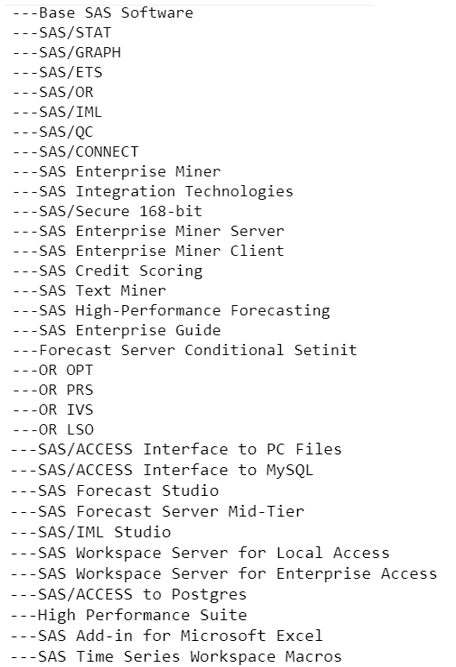
\includegraphics[width=1\linewidth]{img06/w06-SASStudioOnDemand} \end{center}

We will not systematically introduce SAS ODS (Output Delivery System) and ODS graphics, instead, we only demonstrate how to use SAS PROC SGPLOT, PROC SGSCATTER, PROC SGPANEL to create basic statistics graphics such as bar charts, scatter plots, line graphs, etc.

Quite different from the traditional SAS graphics, graphs created with ODS graphics will be in the \texttt{Results\ Window}, not in the \texttt{Graph\ Window}. We can double‐click on the graphics icon to view the file, using a local Windows graphics viewer. Graphs will be automatically saved in .png (portable network graphics) format
files that are
* Raster graphics;
* Compact format;
* Usable in most Windows applications.

For convenience, we still use the penguin data set as our working data set to make various statistics graphics.

\url{https://raw.githubusercontent.com/pengdsci/sta553/main/w02-penguins.csv}

\begin{verbatim}
FILENAME pguin URL "https://raw.githubusercontent.com/pengdsci/sta553/main/w02-penguins.csv";

PROC IMPORT DATAFILE = pguin
    OUT = penguin        
    DBMS = CSV  
    REPLACE;
    GETNAMES = YES;
RUN;

DATA new_penguin;  /* define a new data set */
   SET Penguin;    /* copy the data original data*/
   body_mass = input(body_mass_g, 8.);  /* conversion */
   flipper_length = input(flipper_length_mm, 8.);
   bill_depth = input(bill_depth_mm, 8.);
   bill_length = input(bill_length_mm, 8.);
RUN;
\end{verbatim}

We will only include the minimum graphical features in all graphics. More complex SAS graphics will be discussed later if time permits.

\hypertarget{boxplot}{%
\section{Boxplot}\label{boxplot}}

The box plot is a graphical representation of a five-number summary. It is used to get a rough idea of the distribution of the underlying continuous variable.

\hypertarget{basic-box-plot}{%
\subsection{Basic Box Plot}\label{basic-box-plot}}

The next example draws a basic vertical box plot.

\begin{verbatim}
TITLE "Vertical Box-plot of Body Mass Index";
PROC SGPLOT DATA = new_penguin;
    VBOX body_mass; 
RUN;
\end{verbatim}

\begin{center}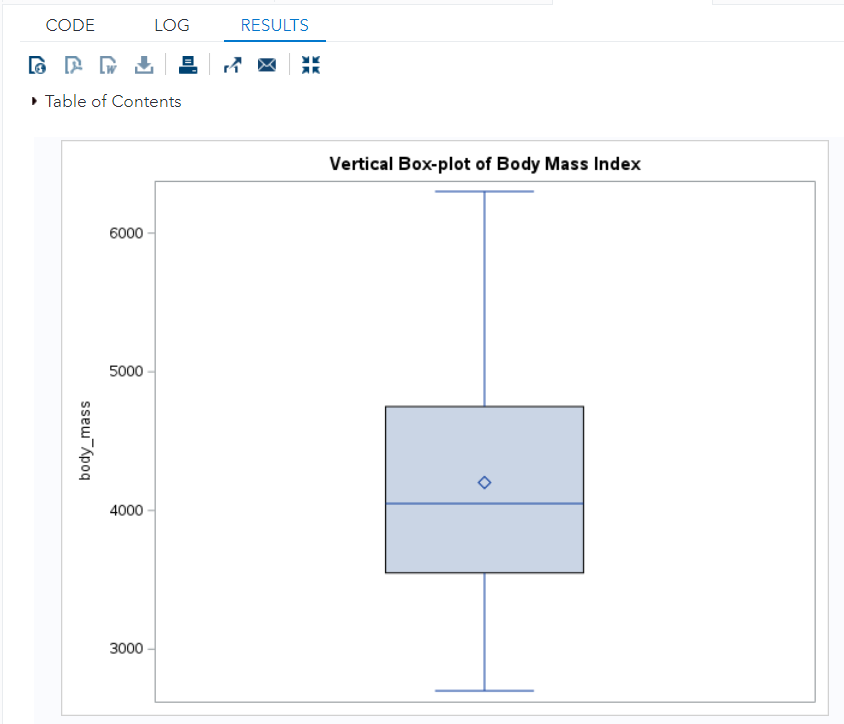
\includegraphics[width=1\linewidth]{img06/w06-Vboxplot} \end{center}

\hypertarget{boxplots-for-categories}{%
\subsection{Boxplots for Categories}\label{boxplots-for-categories}}

If we want to compare the distributions of body mass index among three species of penguins, the following code will create three box plots for comparisons.

\begin{verbatim}
TITLE "Vertical Box-plot of Body Mass Index by species";
PROC SGPLOT DATA = new_penguin;
    VBOX body_mass / category= species; 
RUN;
\end{verbatim}

\begin{center}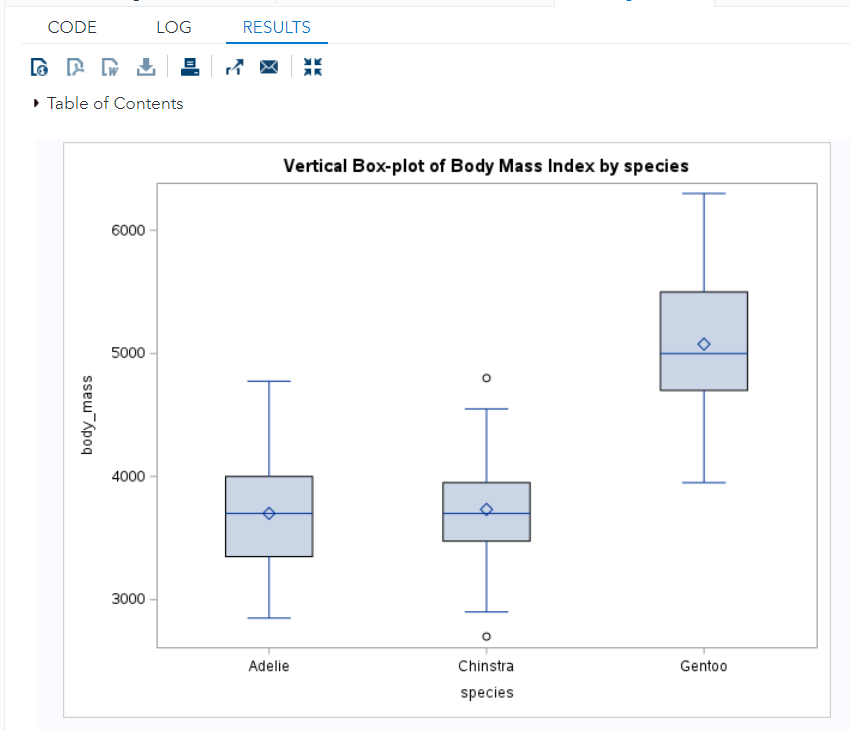
\includegraphics[width=1\linewidth]{img06/w06-BoxplotbySpecies} \end{center}

\hypertarget{panel-box-plot}{%
\subsection{Panel Box Plot}\label{panel-box-plot}}

Further, we could also compare the distribution between \texttt{species} across \texttt{island}. The following panel box plots serve the purpose.

\begin{verbatim}
TITLE "Panel Box-plot of Body Mass Index by species across the islands";
PROC SGPANEL DATA = new_penguin;
    PANELBY island / ROWS = 1 COLUMNS = 3;
    VBOX body_mass / category= species; 
RUN;
\end{verbatim}

\begin{center}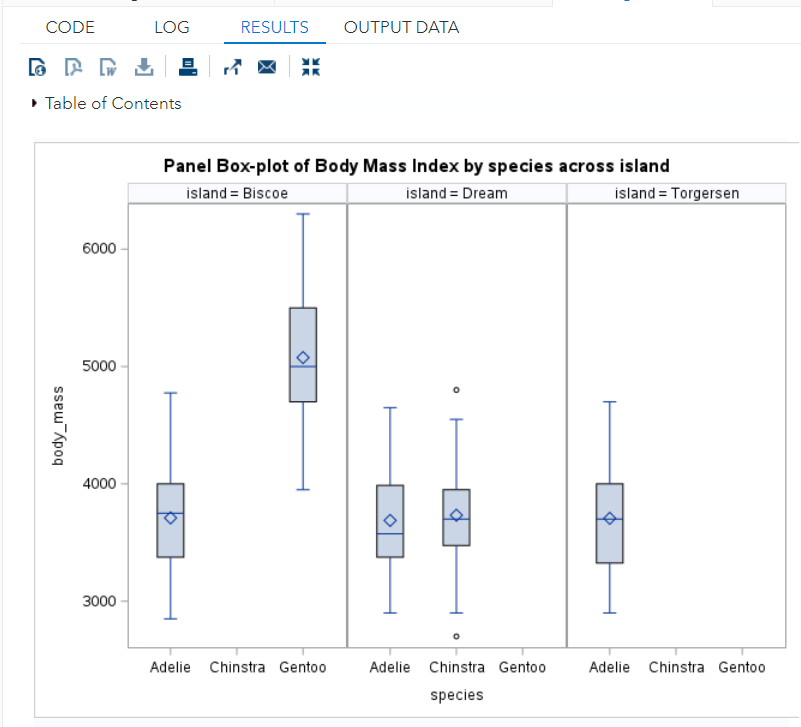
\includegraphics[width=1\linewidth]{img06/w06-PanelBoxPlot} \end{center}

\hypertarget{bar-charts}{%
\section{Bar Charts}\label{bar-charts}}

Bar charts are used to visually display the distribution of categorical variables. This section will illustrate several different bar charts for different purposes. There are three categorical variables in the penguin data set, we will use them in different examples.

\hypertarget{basic-bar-chart-for-one-variable}{%
\subsection{Basic Bar Chart for One Variable}\label{basic-bar-chart-for-one-variable}}

We first make a bar cart for species.

\begin{verbatim}
TITLE "Vertical Baar Chart of Species";
PROC SGPLOT DATA = new_penguin;
    VBAR species; 
RUN;
\end{verbatim}

\begin{center}\includegraphics[width=1\linewidth]{img06/w06-VbarChart} \end{center}

\hypertarget{stacked-bar-charts}{%
\subsection{Stacked Bar Charts}\label{stacked-bar-charts}}

A stacked bar chart can be used to compare the distributions of two categorical variables.

\begin{verbatim}
TITLE "Stacked Bar Chart of Species";
PROC SGPLOT DATA = new_penguin;
    VBAR species/GROUP= sex; 
RUN;
\end{verbatim}

\begin{center}\includegraphics[width=1\linewidth]{img06/w06-stackedBarChart} \end{center}

\hypertarget{bar-charts-with-means-and-error-bars}{%
\subsection{Bar Charts with Means and Error Bars}\label{bar-charts-with-means-and-error-bars}}

In some fields such as health and biological sciences, it is common to visualize means and standard deviations (standard errors) of different groups for comparison. The bar chart of means and errors is the right choice.

\begin{verbatim}
TITLE "Means and Standard Errors by Species";
PROC SGPLOT DATA = new_penguin;
    VBAR species/RESPONSE = body_mass
                 LIMITSTAT = stddev
                 LIMITS = upper 
                 STAT = mean; 
RUN;
\end{verbatim}

\begin{center}\includegraphics[width=1\linewidth]{img06/w06-ErrorBar} \end{center}

\hypertarget{panel-bar-charts}{%
\subsection{Panel Bar Charts}\label{panel-bar-charts}}

Panel bar charts are used to compare means (of a numerical variable) across two categorical variables.

\begin{verbatim}
TITLE "Panel bar chart";
PROC SGPANEL DATA = new_penguin;
    PANELBY sex/ ROWS = 1 COLUMNS = 3;
    VBAR species/RESPONSE = body_mass
                 LIMITSTAT = stddev
                 LIMITS = upper 
                 STAT = mean; 
RUN;
\end{verbatim}

\begin{center}\includegraphics[width=1\linewidth]{img06/w06-PanelBarChart} \end{center}

\hypertarget{histogram}{%
\section{Histogram}\label{histogram}}

A histogram is used to display the distribution of numerical variables. For comparison, it is quite often to overlay two (but rarely more than three) histograms of different numerical variables. In many cases, we also add a density curve on the histogram for comparison (between the estimated density or the reference density function).

\hypertarget{histogram-with-density-curves}{%
\subsection{Histogram with Density Curves}\label{histogram-with-density-curves}}

\begin{verbatim}
PROC SGPLOT DATA = new_penguin;
HISTOGRAM body_mass;
density body_mass;
density body_mass / type = kernel;
keylegend / location=inside position=topright;
RUN;
\end{verbatim}

\begin{center}\includegraphics[width=1\linewidth]{img06/w06-HistDensity} \end{center}

\hypertarget{overlaid-histograms}{%
\subsection{Overlaid Histograms}\label{overlaid-histograms}}

Overlaid histograms are used to compare the distributions of two numerical variables.

\begin{verbatim}
TITLE "Overlaid histogram";
PROC SGPLOT DATA = new_penguin;
HISTOGRAM bill_depth;
HISTOGRAM bill_length / TRANSPARENCY = 0.5;
RUN;
\end{verbatim}

\begin{center}\includegraphics[width=1\linewidth]{img06/w06-OverLaidHist} \end{center}

\hypertarget{panel-histogram}{%
\subsection{Panel Histogram}\label{panel-histogram}}

\begin{verbatim}
TITLE "Histogram with a kernel density curve";
PROC SGPANEL DATA = new_penguin NOAUTOLEGEND;
PANELBY sex / ROWS = 1 COLUMNS = 3;
HISTOGRAM body_mass;
DENSITY body_mass;
DENSITY body_mass / TYPE = kernel;  /* kernel density estimator */
KEYLEGEND / POSITION = BOTTOM;
RUN;
\end{verbatim}

\begin{center}\includegraphics[width=1\linewidth]{img06/w06-PanelHistogram} \end{center}

\hypertarget{scatter-plots}{%
\section{Scatter Plots}\label{scatter-plots}}

A scatter plot of two numerical variables shows the relationship between them. It is quite often that the relationship between numerical variables varies in categories of one or categorical variables. This section displays this kind of relationship between numerical variables under different conditions.

\hypertarget{basic-scatter-plot-for-two-numeric-variables}{%
\subsection{Basic Scatter Plot for Two Numeric Variables}\label{basic-scatter-plot-for-two-numeric-variables}}

\begin{verbatim}
TITLE "Scatter plot of Bill_depth and Bill_length by species";
PROC SGPLOT DATA = new_penguin;
SCATTER x = bill_depth y = bill_length / GROUP = species;
RUN;
\end{verbatim}

\begin{center}\includegraphics[width=1\linewidth]{img06/w06-BasicScatterPlot} \end{center}

The above scatter used color to represent different species.

\hypertarget{scatter-plot-with-least-squares-regression-line}{%
\subsection{Scatter Plot With Least Squares Regression Line}\label{scatter-plot-with-least-squares-regression-line}}

If we simply look at the scatter plot for the over-association between \texttt{bill\_depth} and \texttt{bill\_length}, the pattern is not quite obvious. We may want to add a least regression line to the scatter plot to make it clearer.

\begin{verbatim}
TITLE "Scatter plot of Bill_depth and Bill_length by species";
TITLE2 "with lease square regression line";
PROC SGPLOT DATA = new_penguin;
SCATTER x = bill_depth y = bill_length / GROUP = species;
REG x = bill_depth y = bill_length / cli clm nomarkers;
RUN;
\end{verbatim}

\begin{center}\includegraphics[width=1\linewidth]{img06/w06-ScatterReg} \end{center}

We can see an overall negative correlation between \texttt{bill\_depth} and \texttt{bill\_length}.

\begin{center}\includegraphics[width=0.5\linewidth]{img06/w06-penguinBill} \end{center}

If we look at the same relationship within individual species, the scatter plot shows a positive correlation. We may want to add regression lines to individual species as well to the scatter plot.

\begin{verbatim}
TITLE "Correlation between Bill_depth and Bill_length by species";
TITLE2 "with lease square regression lines";
PROC SGPLOT DATA = new_penguin;
SCATTER x = bill_depth y = bill_length;
REG x = bill_depth y = bill_length / GROUP = species clm;
RUN;
\end{verbatim}

\begin{center}\includegraphics[width=1\linewidth]{img06/w06-IndividualCorrBySpecies} \end{center}

Surprisingly, \texttt{bill\_depth} and \texttt{bill\_length} within each species are all positively correlated which is opposite to what we observed from the overall scatter plot. This pattern is called \textbf{Simpson's paradox} in statistics.

\hypertarget{panel-scatter-plot}{%
\subsection{Panel Scatter Plot}\label{panel-scatter-plot}}

The notion of panel scatter plots is the same. We want to visualize the potential correlation between two \textbf{numerical variables} across the categories of a categorical variable. We have made a single scatter plot and colored different species with different colors. We can also make panel scatter plots such that the scatter plots of individual species are placed in distinct panels.

\begin{verbatim}
TITLE "Panel Scatter Plots: Bill_depth and Bill_length by Species";
TITLE2 "with LOESS smooth curves";
PROC SGPANEL DATA = new_penguin;
  PANELBY species/ROWS = 1 COLUMNS = 3;
  SCATTER x = bill_depth y = bill_length/ GROUP = species;
  LOESS x = bill_depth y = bill_length; 
RUN;
\end{verbatim}

\begin{center}\includegraphics[width=1\linewidth]{img06/w06-panelScatterWithLoess} \end{center}

\hypertarget{pair-wise-scatter-plot}{%
\section{Pair-wise Scatter Plot}\label{pair-wise-scatter-plot}}

It is useful to visually inspect the potential high correlation between \textbf{numerical variables} (usually three or more) in regression modeling to see the potential impact of (pair-wise) collinearity (not the multicollinearity).

For illustration, we use the 4 numerical variables in the \texttt{new\_penguin} data set to make a pair-wise scatter plot.

\begin{verbatim}
TITLE "Pair-wise Scatter Plot";
TITLE2 "Penguins on Biscoe Island";
PROC SGSCATTER DATA = new_penguin;
WHERE island = 'Biscoe';
MATRIX bill_depth bill_length flipper_length 
      body_mass / GROUP = species 
                  DIAGONAL=(HISTOGRAM KERNEL);
RUN;
\end{verbatim}

\begin{center}\includegraphics[width=1\linewidth]{img06/w06-PairWiseScatter} \end{center}

\hypertarget{learning-coding-by-examples-2}{%
\section{Learning Coding by Examples}\label{learning-coding-by-examples-2}}

This section provides more examples that use more SAS graphical statements to improve the previously introduced statistics graph aesthetically.

For convenience, we use the SAS built-in data set in the following examples.

\begin{verbatim}
/***************************************************
        High-Quality Statistical Plots - SGPLOT
  Topics:   1 - Histograms
            2 - Barcharts
            3 - Scatter Plots          
            4 - Box-plots
            5 - Simple Linear Regression Lines
            6 - Density Curves
***************************************************/

DM "CLEAR OUT";
DM "CLEAR LOG";

/***  Permanent library  ***/
LIBNAME sgplot "C:\STA311\w06";   
/* permanent library for saving SAS data related to PROC SGPLOT  */

/** Global options for outputs **/
OPTIONS PS = 76 LS = 76 NONUMBER NODATE;

/****************************************
   Review: Loading SAS data set to SAS
*****************************************/

/** Have to use library reference to access
    any SAS data sets and load them to SAS  */

DATA sgplot.myAirDataSet;
SET sashelp.Air;    /* This is a SAS built-in data set*/
RUN;

DATA work.myWorkAirData;
SET sgplot.myAirDataSet;
RUN;

/***********************************
***   Explore car.sas7bdat
************************************/
TITLE "SAS Built-in Data Set: cars.sas7bdat";   
                  /* global option. Keep in mind that this title should be 
                     updated appropriately according to the new output*/
PROC CONTENTS DATA = sashelp.cars;     
                  /* sashelp is the library reference to the SAS built-in 
                     permanent library */
RUN;              /* IMPORTANT: If you want to load a SAS data set to SAS 
                     from a folder, you should always create an SAS permanent 
                     library pointing to the folder, then use the library 
                     reference and SAS data or procedure steps to access the SAS
                     format data.  */

/************************
** Topic 1: Histogram
*************************/

* Example 1.0 - basic histogram;
PROC SGPLOT DATA = Sashelp.cars;
 HISTOGRAM MSRP;        /* The default histogram is based on the relative 
                           frequency table */
 TITLE "The Simplest Histogram of MSRP";
RUN; 


/********************************************************************* 
Example 1.1. Histogram with more controls by specifying options.
               The syntax is: HISTOGRAM MSRP/<options>
               Available options can be found on the SAS web page

**********************************************************************/

ODS GRAPHICS ON / WIDTH = 4.5IN HEIGHT = 3.5IN;  
                                   /* control the size of the SAS graphic */
PROC SGPLOT DATA = Sashelp.cars;
 HISTOGRAM MSRP/ NBINS = 6         /* 6 vertical bars are requested. */
                 SCALE = count     /* Default scale is percent */
                         Y2AXIS            /* draw two vertical axes */
                         DATASKIN = GLOSS; /* effects of vertical bars */
                                
 TITLE "Histogram of MSRP with more controls";
RUN; 
ODS GRAPHICS OFF;


/* Example 1.3 - histogram with a density curve: 
   i.e., stack one curve on the other; */
   
ODS GRAPHICS ON / WIDTH = 4.5IN HEIGHT = 3.5IN;   
                      /** control the size of the SAS graphic  **/
PROC SGPLOT DATA = Sashelp.cars;
  HISTOGRAM MSRP;   /* use the default number of vertical bars */
  DENSITY MSRP;     /* By default, a default density curve is normal: 
                      mu = sample mean, sd = sample std 
                      you can also choose KERNEL option --> 
                      data driven density estimator.           */
 TITLE "Histogram of MSRP with Density Curve";
RUN; 
ODS GRAPHICS OFF;

/************************
** Topic 2: Bar Charts
*************************/

* Example 2.1 Basic Bar Charts;
ODS GRAPHICS ON / WIDTH = 4.5IN HEIGHT = 3.5IN;    
PROC SGPLOT DATA = Sashelp.cars;
 VBAR Type;     /* name of character variable used in the bar chart */        
 TITLE 'Barchart of Type of Vehicles';
RUN;
ODS GRAPHICS OFF;

/* Example 2.2 - bar chart by the origin ; */
ODS GRAPHICS ON / WIDTH = 4.5IN HEIGHT = 3.5IN;  
PROC SGPLOT DATA = Sashelp.cars;
 HBAR Type / GROUP = Origin;
 TITLE 'Barchart of Type by the origin';
RUN; 
ODS GRAPHICS OFF;

*Example 2.3 - Response option  ;
DATA temp_cars;
  SET Sashelp.cars;
  counter = 1;   /* add a new constant variable to the SAS data  */
RUN;

/* We use the counter as a response variable   */
ODS GRAPHICS ON / WIDTH = 4.5IN HEIGHT = 3.5IN;
PROC SGPLOT DATA = temp_cars;
 VBAR Type / RESPONSE = counter;
              /* RESPOSE option adds up all values of the variable 
                 counter in each category of the categorical variable Type. 
                The resulting bar chart is the same as the regular bar chart */
 TITLE 'Barchart - bar';
RUN; 
ODS GRAPHICS OFF;

/****************************************
**  Topic 3:  Scatter plot 
*****************************************/
* Example 3.1 - scatter plot - basic;
ODS GRAPHICS ON / WIDTH = 4.5IN HEIGHT = 3.5IN;
PROC SGPLOT DATA = Sashelp.cars;
 SCATTER X = MSRP Y = invoice;  
        /* It doesn't matter which variable is X and which is Y. */
 TITLE 'Scatter plot of MSRP vs Invoices';
RUN; 
ODS GRAPHICS OFF;

* Example 3.2 - scatter plot - by groups
  PROC SGPanel - allows making each for each category of the categorical 
                 the variable specified in the PANELBY statement;

ODS GRAPHICS ON / WIDTH = 4.5IN HEIGHT = 3.5IN;
PROC SGPANEL DATA = Sashelp.cars;
 PANELBY Type;      /* The  */
 SCATTER X = MPG_Highway Y = MPG_City;
 TITLE 'Line plot of MSRP vs Invoices';
RUN; 
ODS GRAPHICS OFF;

* plot matrix: plot    ;
TITLE "Scatter Plot Matrix Several Continuous Variables in CARS";
ODS GRAPHICS ON / WIDTH = 4.5IN HEIGHT = 3.5IN;
PROC SGSCATTER DATA =Sashelp.cars;
MATRIX MSRP INVOICE HORSEPOWER 
       MPG_CITY MPG_HIGHWAY / TRANSPARENCY = 0.6  
                              /* degree of transparency of the plot */
                              ELLIPSE   /* Add an ellipse to the data points 
                                           to visualize the strength of 
                                           the association between the two
            variables.*/
                              MARKERATTRS =(symbol=circlefilled)
                              DIAGONAL=(histogram normal kernel);
RUN;
ODS GRAPHICS OFF;


/*************************************
**   Topic 4: Box-plots
**************************************/

/** Example 4.1 Simple box-plot **/
TITLE 'Distribution of Mileage';
ODS GRAPHICS ON / WIDTH =4.5IN HEIGHT=3.5IN;
PROC SGPLOT DATA =sashelp.cars noautolegend;
HBOX mpg_city ;     /* Horizontal box-plot */
YAXIS GRID;  /* DISPLAY is not specified. The default value of 
                DISPLAY = (all): ticks, label and values are all displayed */
XAXIS DISPLAY = (nolabel);   /* only the x-label is not displayed  */
RUN;
ODS GRAPHICS OFF;


/** Example 4.2: Box-plot - by type  **/
ODS GRAPHICS ON / WIDTH =4.5IN HEIGHT=3.5IN;
TITLE 'Distribution of Mileage by Type';
PROC SGPLOT DATA =sashelp.cars noautolegend;
HBOX mpg_city / CATEGORY =type;
YAXIS GRID; 
XAXIS DISPLAY = (nolabel);
RUN;
ODS GRAPHICS OFF;

/** 4.3. Box-plot with a line plot connecting means  **/
TITLE 'Mileage by Type';
ODS GRAPHICS ON / WIDTH =4.5IN HEIGHT=3.5IN;   
                 /** control the size of the graphic  **/
PROC SGPLOT DATA =sashelp.cars;
/* vertical box-plot, opposed to horizontal box-plot with HBOX option */
VBOX mpg_city / CATEGORY =type  /* The categorical to be used to  */
                CONNECT = mean  /* connect the specified quantities of 
                                  each category with a line segment */
                DATALABEL;      /* use observation ID of the data value 
                                 if the value is an outlier      */
XAXIS GRID DISPLAY = (noticks nolabel); /* whether ticks, label, values 
                                          associated with the axis are displayed*/
YAXIS GRID DISPLAY = (novalues nolabel);
RUN;
ODS GRAPHICS OFF; 

/** Example 4.4. Multiple box-plots on the same plot   **/
PROC SGPLOT DATA =sashelp.cars;
 VBOX enginesize / CATEGORY=type     /* Make a box plot for each category 
                                        of the character variable*/
                   BOXWIDTH=0.25     /* box width of the box-plot */
                   DISCRETEOFFSET = -0.15; /* the deviation of box-plot 
                                              associated with variable 
                                              enginesize to the left of 
                                              the center of the category */
  VBOX horsepower / CATEGORY=type 
                   BOXWIDTH=0.25 
                   DISCRETEOFFSET=0.15  /* the deviation of the box-plot associated 
                                           with variable enginesize to the 
                                           right of the center of the category.
                                                   The distance between the two 
                                                   box-plots is 0.15-(-0.15) = 0.3 */
    2AXIS;                /* Make two vertical axes since two numerical 
                             variables are at different scales!   */
RUN;


/*************************************
**   Topic 5: Regression Line
**************************************/

/* Example 5.1. Scatter plot with a regression line  */
TITLE "Scatter Plot with Regression Line";
PROC SGPLOT DATA = sashelp.cars;
REG y = Horsepower x=Weight; /* y = response var, x = horizontal var */
RUN;


/** Example 5.2. Regression with confidence limits **/
TITLE1 "Scatter Plot with Regression Line";
TITLE2 "with Confidence Limits/Band";
PROC SGPLOT DATA = sashelp.cars;
REG y = Horsepower x=Weight/ CLI   /* confidence limits of individual 
                                      predicted values */
                             CLM   /* confidence limit of the regression line 
                                      - confidence band */
                             alpha=0.1;  /* confidence level = 1 - 0.1 = 90%, 
                                            default ALPHA = 0.05  */
RUN;

/** Example 5.3. Regression with confidence limits **/
TITLE1 "Scatter Plot with Regression Line";
TITLE2 "with Confidence Limits/Band, line/marker attributes";
PROC SGPLOT DATA = sashelp.cars;
REG y = Horsepower x=Weight/ CLI         
                             CLM         
                             alpha=0.1   
                             lineattrs=(color=red thickness=5)
                             markerattrs=(color=blue size=10
                             symbol=squarefilled);
RUN;


/*************************************
** Topic 6: Density function 
**************************************/

/* Example 6.1. calculate the mean and standard deviation and then use
   the mean and standard deviation to fit a normal distribution.
   The density curve will be placed on the histogram*/

TITLE 'Normal Density for Horsepower';
ODS GRAPHICS ON / WIDTH = 4.5IN HEIGHT = 3.5IN;
PROC SGPLOT DATA=sashelp.cars NOAUTOLEGEND;  /* NOAUTOLEGEND: disables automatic 
                                                legends from being generated.  */
HISTOGRAM HORSEPOWER;
DENSITY HORSEPOWER;
YAXIS GRID; 
XAXIS DISPLAY = (nolabel);  /* X-axis label is disabled. */
RUN;
ODS GRAPHICS OFF;

/**Example 6.2: Use a different variable: MSRP  **/
TITLE 'Normal Density for MSRP';
ODS GRAPHICS ON / WIDTH = 4.5IN HEIGHT = 3.5IN;
PROC SGPLOT DATA=sashelp.cars NOAUTOLEGEND; 
              /* By default, legends are created automatically for some plots, 
                 depending on their content. This option has no effect 
                 if you specify a KEYLEGEND statement. */
HISTOGRAM MSRP;
DENSITY MSRP;
YAXIS GRID; 
XAXIS DISPLAY = (nolabel);   /* X-axis label is disabled. */
RUN;
ODS GRAPHICS OFF;

/** Example 6.3: kernel density curve **/
TITLE 'Normal Density for MSRP';
ODS GRAPHICS ON / WIDTH = 4.5IN HEIGHT = 3.5IN;
PROC SGPLOT DATA=sashelp.cars; *NOAUTOLEGEND;
HISTOGRAM MSRP / SCALE = percent;
DENSITY MSRP / SCALE = percent 
               TYPE = Kernel;
YAXIS GRID; 
XAXIS DISPLAY = (nolabel);
RUN;
ODS GRAPHICS OFF;

/** Example 6.4. Kernel and normal density  **/
TITLE 'Normal/Kernel Density for MSRP';
ODS GRAPHICS ON / WIDTH = 4.5IN HEIGHT = 3.5IN;
PROC SGPLOT DATA=sashelp.cars;
HISTOGRAM MSRP / SCALE = percent;   /* percent = relative frequency, 
                                       This is the default scale in SAS */
DENSITY MSRP;     
DENSITY MSRP / TYPE = Kernel;
KEYLEGEND / LOCATION =inside 
            POSITION = topright 
            ACROSS = 1;
YAXIS GRID DISPLAY = (nolabel); 
XAXIS GRID DISPLAY = (nolabel);
RUN;
ODS GRAPHICS OFF;
\end{verbatim}

\hypertarget{subsetting-data}{%
\chapter{Subsetting Data}\label{subsetting-data}}

\textbf{Subsetting Data} is a process of creating a smaller data set based on a larger data set. There are major methods for subsetting a data set: selecting and splitting.

\begin{itemize}
\item
  Selecting: We \textbf{select/keep} rows and columns from a data set to make a smaller data set. We can also \textbf{delete} rows and \textbf{drop} columns to make a smaller data set.
\item
  Splitting: From the self-explanatory term, we can split a larger data set into several smaller data sets.
\end{itemize}

This chapter discusses the above different methods with some examples. We will still use the penguin data set in illustrative examples.

\url{https://raw.githubusercontent.com/pengdsci/sta553/main/w02-penguins.csv}

\begin{verbatim}
FILENAME pguin URL "https://raw.githubusercontent.com/pengdsci/sta553/main/w02-penguins.csv";

PROC IMPORT DATAFILE = pguin
    OUT = penguin        
    DBMS = CSV  
    REPLACE;
    GETNAMES = YES;
RUN;

DATA new_penguin;  /* define a new data set */
   SET Penguin;    /* copy the data original data*/
   body_mass = input(body_mass_g, 8.);  /* conversion */
   flipper_length = input(flipper_length_mm, 8.);
   bill_depth = input(bill_depth_mm, 8.);
   bill_length = input(bill_length_mm, 8.);
RUN;
\end{verbatim}

\begin{center}\includegraphics[width=1\linewidth]{img07/w07-penguinContents} \end{center}

\hypertarget{selecting-columns}{%
\section{Selecting Columns}\label{selecting-columns}}

This subsetting method is straightforward. SAS statements \textbf{KEEP} and \textbf{DROP} to define a smaller data set.

The \texttt{new\_penguin} is defined based on the original \texttt{penguin} data set in which all numerical variables were defined in character form. We converted four character-encoded variables into numerical variables and added them to \texttt{penguin} with new names.

We now drop variables \texttt{bill\_depth\_mm}, \texttt{bill\_length\_mm}, \texttt{body\_mass\_g}, and \texttt{flipper\_length\_mm} from the data set \texttt{new\_penguin} and only keep only numerical version of these variables.

\begin{verbatim}
DATA penguin01;
  SET new_penguin;
  DROP bill_depth_mm bill_length_mm body_mass_g flipper_length_mm;
RUN;

PROC CONTENTS DATA = penguin01;
RUN;
\end{verbatim}

\begin{center}\includegraphics[width=1\linewidth]{img07/w07-penguin01Contents} \end{center}

We can also use \texttt{KEEP} statement to subset the data set.

\begin{verbatim}
DATA penguin02;
  SET new_penguin;
  KEEP bill_depth 
  bill_length 
  body_mass 
  flipper_length
  island
  sex
  species
  year;
RUN;

PROC CONTENTS DATA = penguin02;
RUN;
\end{verbatim}

\begin{center}\includegraphics[width=1\linewidth]{img07/w07-penguin02Contents} \end{center}

\hypertarget{selecting-rows}{%
\section{Selecting Rows}\label{selecting-rows}}

Selecting columns is relatively straightforward. Working with rows is challenging since there are different ways of selecting rows under certain conditions.

\hypertarget{partial-reading}{%
\subsection{Partial Reading}\label{partial-reading}}

Sometimes file movements have a size limit. For example, the file size in an email attachment should not be bigger than, say 15MB. If you have a 25 MB data file, we can use \texttt{OBS=} to read part of the data file and create two smaller data files.

We have used \texttt{OBS\ =} and \texttt{FIRSTOBS\ =} in the previous chapter to read a data file with descriptions and comments.

For example, we now define a data set by including observations 100 - 200 in the \texttt{penguin02}.

\begin{verbatim}
DATA penguin03;
SET penguin02(FIRSTOBS = 100 OBS = 200);
RUN;

PROC CONTENTS DATA = penguin03;
RUN;
\end{verbatim}

\begin{center}\includegraphics[width=1\linewidth]{img07/w07-penguin03Contents} \end{center}

\hypertarget{conditional-selecting-methods}{%
\subsection{Conditional Selecting Methods}\label{conditional-selecting-methods}}

This type of method uses conditional statements to select rows. Three keywords \texttt{WHERE}, \texttt{IF-THEN}, and \texttt{IN} are used to define conditions for selecting rows.

\hypertarget{where-and-in}{%
\subsubsection{\texorpdfstring{\texttt{WHERE} and \texttt{IN}}{WHERE and IN}}\label{where-and-in}}

We have used \texttt{WHERE} in the previous chapter on SAS graphics. For example, we create a subset that contains two of the three \texttt{species}: \emph{Chinstra} and \emph{Gentoo}.

\begin{verbatim}
DATA penguin04;
  SET penguin02;
  WHERE (species = 'Chinstra' OR species = 'Gentoo');
RUN;

PROC FREQ DATA = penguin04;
TABLE species;
TITLE "Checking species in the new subset";
RUN;
title ""
\end{verbatim}

\begin{center}\includegraphics[width=1\linewidth]{img07/w07-penguinSpeciesWHERE} \end{center}

We can see that \texttt{WHERE} successfully subsets the data. We can also use \texttt{IN} statement to perform the same task.

\begin{verbatim}
DATA penguin04;
  SET penguin02;
  WHERE species IN ('Chinstra' 'Gentoo');
RUN;

PROC FREQ DATA = penguin04;
TABLE species;
TITLE " WHERE-IN: species in the new subset";
RUN;
title ""
\end{verbatim}

\begin{center}\includegraphics[width=1\linewidth]{img07/w07-penguinSpeciesWHERE-IN} \end{center}

\hypertarget{if-then-delete}{%
\subsubsection{\texorpdfstring{\texttt{IF-THEN-DELETE}}{IF-THEN-DELETE}}\label{if-then-delete}}

We can also delete those rows that we don't want to include in the final subset by using the statement \texttt{IF-THEN-DELETE}. We next create the above data set \texttt{penguin05} by deleting species \emph{Adelie}

\begin{verbatim}
DATA penguin05;
  SET penguin02;
  IF species = 'Adelie' THEN DELETE;
RUN;

PROC FREQ DATA = penguin05;
TABLE species;
TITLE " IF-THEN-DELETE: species in the new subset";
RUN;
title ""
\end{verbatim}

\begin{center}\includegraphics[width=1\linewidth]{img07/w07-penguinSpeciesIF_THEN_DELETE} \end{center}

\hypertarget{subsetting-by-splitting}{%
\section{Subsetting by Splitting}\label{subsetting-by-splitting}}

We can split a large data set into several small data sets by using the conditional statement \texttt{IF-THEN-OUTPUT}. This allows us to define several subsets in a single data step. The next example shows how the split \texttt{penguin02} into three subsets and each subset contains only one species.

\begin{verbatim}
DATA Adelie Chinstra Gentoo;
  SET penguin02;
  IF species = 'Adelie' THEN OUTPUT Adelie;
  IF species = 'Chinstra' THEN OUTPUT Chinstra;
  IF species = 'Gentoo' THEN OUTPUT Gentoo;
RUN;
\end{verbatim}

\begin{center}\includegraphics[width=1\linewidth]{img07/w07-IT_THEN_OUT-log} \end{center}

The above log file indicates that three subsets are successfully defined.

\hypertarget{learning-coding-by-examples-3}{%
\section{Learning Coding by Examples}\label{learning-coding-by-examples-3}}

This section provides numerous examples using different methods to subset data. One of the working data sets can be found at
\url{https://raw.githubusercontent.com/pengdsci/STA311/main/w07-us-counties.csv}

The last example uses automatic variables to subset data.

\begin{verbatim}
/***************************************************************
             Subsetting and Splitting Data Sets

          Topics 1. Subsetting Datasets by Conditional Processing
                 2. Subsetting Datasets by Rows
                 3. Splitting a Dataset
                 4. Subsetting Variables
                 5. Subsetting Rows with Auto Variables
***************************************************************/

DM "CLEAR LOG";
DM "CLEAR OUT";

OPTIONS PS = 76 LS = 76 NONUMBER NODATE;

LIBNAME w07 "C:\STA311\w07";

/*************************************************
This session focuses on subsetting SAS data sets
using SAS keywords and SAS conditional statements. 
Most of the examples will be based on the following 
two working data sets.
**************************************************/


/***********************************/
/*       Working data set #1       */
/***********************************/

DATA auto ;
  LENGTH make $ 20 ;
  INPUT make $ 1-17 
        price 
        mpg 
        rep78 
        hdroom 
        trunk 
        weight 
        length 
        turn
        displ 
        gratio 
        foreign ;
DATALINES;
AMC Concord        4099 22 3 2.5 11 2930 186 40 121 3.58 0
AMC Pacer          4749 17 3 3.0 11 3350 173 40 258 2.53 0
AMC Spirit         3799 22 . 3.0 12 2640 168 35 121 3.08 0
Audi 5000          9690 17 5 3.0 15 2830 189 37 131 3.20 1
Audi Fox           6295 23 3 2.5 11 2070 174 36  97 3.70 1
BMW 320i           9735 25 4 2.5 12 2650 177 34 121 3.64 1
Buick Century      4816 20 3 4.5 16 3250 196 40 196 2.93 0
Buick Electra      7827 15 4 4.0 20 4080 222 43 350 2.41 0
Buick LeSabre      5788 18 3 4.0 21 3670 218 43 231 2.73 0
Buick Opel         4453 26 . 3.0 10 2230 170 34 304 2.87 0
Buick Regal        5189 20 3 2.0 16 3280 200 42 196 2.93 0
Buick Riviera     10372 16 3 3.5 17 3880 207 43 231 2.93 0
Buick Skylark      4082 19 3 3.5 13 3400 200 42 231 3.08 0
Cad. Deville      11385 14 3 4.0 20 4330 221 44 425 2.28 0
Cad. Eldorado     14500 14 2 3.5 16 3900 204 43 350 2.19 0
Cad. Seville      15906 21 3 3.0 13 4290 204 45 350 2.24 0
Chev. Chevette     3299 29 3 2.5  9 2110 163 34 231 2.93 0
Chev. Impala       5705 16 4 4.0 20 3690 212 43 250 2.56 0
Chev. Malibu       4504 22 3 3.5 17 3180 193 31 200 2.73 0
Chev. Monte Carlo  5104 22 2 2.0 16 3220 200 41 200 2.73 0
Chev. Monza        3667 24 2 2.0  7 2750 179 40 151 2.73 0
Chev. Nova         3955 19 3 3.5 13 3430 197 43 250 2.56 0
Datsun 200         6229 23 4 1.5  6 2370 170 35 119 3.89 1
Datsun 210         4589 35 5 2.0  8 2020 165 32  85 3.70 1
Datsun 510         5079 24 4 2.5  8 2280 170 34 119 3.54 1
Datsun 810         8129 21 4 2.5  8 2750 184 38 146 3.55 1
Dodge Colt         3984 30 5 2.0  8 2120 163 35  98 3.54 0
Dodge Diplomat     4010 18 2 4.0 17 3600 206 46 318 2.47 0
Dodge Magnum       5886 16 2 4.0 17 3600 206 46 318 2.47 0
Dodge St. Regis    6342 17 2 4.5 21 3740 220 46 225 2.94 0
Fiat Strada        4296 21 3 2.5 16 2130 161 36 105 3.37 1
Ford Fiesta        4389 28 4 1.5  9 1800 147 33  98 3.15 0
Ford Mustang       4187 21 3 2.0 10 2650 179 43 140 3.08 0
Honda Accord       5799 25 5 3.0 10 2240 172 36 107 3.05 1
Honda Civic        4499 28 4 2.5  5 1760 149 34  91 3.30 1
Linc. Continental 11497 12 3 3.5 22 4840 233 51 400 2.47 0
Linc. Mark V      13594 12 3 2.5 18 4720 230 48 400 2.47 0
Linc. Versailles  13466 14 3 3.5 15 3830 201 41 302 2.47 0
Mazda GLC          3995 30 4 3.5 11 1980 154 33  86 3.73 1
Merc. Bobcat       3829 22 4 3.0  9 2580 169 39 140 2.73 0
Merc. Cougar       5379 14 4 3.5 16 4060 221 48 302 2.75 0
Merc. Marquis      6165 15 3 3.5 23 3720 212 44 302 2.26 0
Merc. Monarch      4516 18 3 3.0 15 3370 198 41 250 2.43 0
Merc. XR-7         6303 14 4 3.0 16 4130 217 45 302 2.75 0
Merc. Zephyr       3291 20 3 3.5 17 2830 195 43 140 3.08 0
Olds 98            8814 21 4 4.0 20 4060 220 43 350 2.41 0
Olds Cutl Supr     5172 19 3 2.0 16 3310 198 42 231 2.93 0
Olds Cutlass       4733 19 3 4.5 16 3300 198 42 231 2.93 0
Olds Delta 88      4890 18 4 4.0 20 3690 218 42 231 2.73 0
Olds Omega         4181 19 3 4.5 14 3370 200 43 231 3.08 0
Olds Starfire      4195 24 1 2.0 10 2730 180 40 151 2.73 0
Olds Toronado     10371 16 3 3.5 17 4030 206 43 350 2.41 0
Peugeot 604       12990 14 . 3.5 14 3420 192 38 163 3.58 1
Plym. Arrow        4647 28 3 2.0 11 3260 170 37 156 3.05 0
Plym. Champ        4425 34 5 2.5 11 1800 157 37  86 2.97 0
Plym. Horizon      4482 25 3 4.0 17 2200 165 36 105 3.37 0
Plym. Sapporo      6486 26 . 1.5  8 2520 182 38 119 3.54 0
Plym. Volare       4060 18 2 5.0 16 3330 201 44 225 3.23 0
Pont. Catalina     5798 18 4 4.0 20 3700 214 42 231 2.73 0
Pont. Firebird     4934 18 1 1.5  7 3470 198 42 231 3.08 0
Pont. Grand Prix   5222 19 3 2.0 16 3210 201 45 231 2.93 0
Pont. Le Mans      4723 19 3 3.5 17 3200 199 40 231 2.93 0
Pont. Phoenix      4424 19 . 3.5 13 3420 203 43 231 3.08 0
Pont. Sunbird      4172 24 2 2.0  7 2690 179 41 151 2.73 0
Renault Le Car     3895 26 3 3.0 10 1830 142 34  79 3.72 1
Subaru             3798 35 5 2.5 11 2050 164 36  97 3.81 1
Toyota Celica      5899 18 5 2.5 14 2410 174 36 134 3.06 1
Toyota Corolla     3748 31 5 3.0  9 2200 165 35  97 3.21 1
Toyota Corona      5719 18 5 2.0 11 2670 175 36 134 3.05 1
Volvo 260         11995 17 5 2.5 14 3170 193 37 163 2.98 1
VW Dasher          7140 23 4 2.5 12 2160 172 36  97 3.74 1
VW Diesel          5397 41 5 3.0 15 2040 155 35  90 3.78 1
VW Rabbit          4697 25 4 3.0 15 1930 155 35  89 3.78 1
VW Scirocco        6850 25 4 2.0 16 1990 156 36  97 3.78 1
;
RUN;

PROC CONTENTS DATA=auto;
RUN;

/***********************************/
/*       Working data set #2       */
/*         NYT COVID-19            */
/***********************************/
PROC IMPORT OUT= WORK.us_county_covid19 
            DATAFILE= "C:\STA311\w07\w07-us-counties.csv" 
            DBMS=CSV REPLACE;
     GETNAMES=YES;
     GUESSINGROWS=3000; /* Caution: if omitted, the default is 20 */
     DATAROW=2; 
RUN;

PROC CONTENTS DATA = us_county_covid19;
RUN;

/**************************************************
  Topic #1: Subsetting Datasets by Conditions
      Conditional keywords:
      1. IF
      2. IF-THEN-DELETE
      3. IF-THEN-OUTPUT 
      4. WHERE
***************************************************/

PROC CONTENTS DATA = auto;
RUN;


/* IF condition */
DATA FOREIN_CARS01;
SET AUTO;      /* SAS data set */
IF FOREIGN =1;  /* foreign = 1 (foreign), 0 (domestic) */
RUN;


/* IF-THEN-DELETE */
DATA FOREIGN_CARS02;
SET AUTO;
IF FOREIGN = 0 THEN DELETE; /* deleting domestic cars */
RUN;


/*  IF-THEN-OUTPUT  */
DATA FOREIGN_CARS03;
SET AUTO;
IF FOREIGN =1 THEN OUTPUT;
RUN;


/*  WHERE  */
DATA FOREIGN_CARS04;
SET AUTO;
WHERE FOREIGN = 1;
RUN;

/* IF statement can also be used in the data input step after 
   INPUT statement. However, WHERE can not be used
   before the SAS data set is created,                    */

DATA FOREIGN_CARS05 ;
  LENGTH make $ 20 ;
  INPUT make $ 1-17 price mpg rep78 hdroom trunk weight length turn
        displ gratio foreign ;
  IF FOREIGN =1;  /*  WHERE does not work with INPUT statement  */
DATALINES;
AMC Concord        4099 22 3 2.5 11 2930 186 40 121 3.58 0
AMC Pacer          4749 17 3 3.0 11 3350 173 40 258 2.53 0
AMC Spirit         3799 22 . 3.0 12 2640 168 35 121 3.08 0
Audi 5000          9690 17 5 3.0 15 2830 189 37 131 3.20 1
Audi Fox           6295 23 3 2.5 11 2070 174 36  97 3.70 1
BMW 320i           9735 25 4 2.5 12 2650 177 34 121 3.64 1
Buick Century      4816 20 3 4.5 16 3250 196 40 196 2.93 0
Buick Electra      7827 15 4 4.0 20 4080 222 43 350 2.41 0
Buick LeSabre      5788 18 3 4.0 21 3670 218 43 231 2.73 0
Buick Opel         4453 26 . 3.0 10 2230 170 34 304 2.87 0
Buick Regal        5189 20 3 2.0 16 3280 200 42 196 2.93 0
Buick Riviera     10372 16 3 3.5 17 3880 207 43 231 2.93 0
Buick Skylark      4082 19 3 3.5 13 3400 200 42 231 3.08 0
Cad. Deville      11385 14 3 4.0 20 4330 221 44 425 2.28 0
Cad. Eldorado     14500 14 2 3.5 16 3900 204 43 350 2.19 0
Cad. Seville      15906 21 3 3.0 13 4290 204 45 350 2.24 0
Chev. Chevette     3299 29 3 2.5  9 2110 163 34 231 2.93 0
Chev. Impala       5705 16 4 4.0 20 3690 212 43 250 2.56 0
Chev. Malibu       4504 22 3 3.5 17 3180 193 31 200 2.73 0
Chev. Monte Carlo  5104 22 2 2.0 16 3220 200 41 200 2.73 0
Chev. Monza        3667 24 2 2.0  7 2750 179 40 151 2.73 0
Chev. Nova         3955 19 3 3.5 13 3430 197 43 250 2.56 0
Datsun 200         6229 23 4 1.5  6 2370 170 35 119 3.89 1
Datsun 210         4589 35 5 2.0  8 2020 165 32  85 3.70 1
Datsun 510         5079 24 4 2.5  8 2280 170 34 119 3.54 1
Datsun 810         8129 21 4 2.5  8 2750 184 38 146 3.55 1
Dodge Colt         3984 30 5 2.0  8 2120 163 35  98 3.54 0
Dodge Diplomat     4010 18 2 4.0 17 3600 206 46 318 2.47 0
Dodge Magnum       5886 16 2 4.0 17 3600 206 46 318 2.47 0
Dodge St. Regis    6342 17 2 4.5 21 3740 220 46 225 2.94 0
Fiat Strada        4296 21 3 2.5 16 2130 161 36 105 3.37 1
Ford Fiesta        4389 28 4 1.5  9 1800 147 33  98 3.15 0
Ford Mustang       4187 21 3 2.0 10 2650 179 43 140 3.08 0
Honda Accord       5799 25 5 3.0 10 2240 172 36 107 3.05 1
Honda Civic        4499 28 4 2.5  5 1760 149 34  91 3.30 1
Linc. Continental 11497 12 3 3.5 22 4840 233 51 400 2.47 0
Linc. Mark V      13594 12 3 2.5 18 4720 230 48 400 2.47 0
Linc. Versailles  13466 14 3 3.5 15 3830 201 41 302 2.47 0
Mazda GLC          3995 30 4 3.5 11 1980 154 33  86 3.73 1
Merc. Bobcat       3829 22 4 3.0  9 2580 169 39 140 2.73 0
Merc. Cougar       5379 14 4 3.5 16 4060 221 48 302 2.75 0
Merc. Marquis      6165 15 3 3.5 23 3720 212 44 302 2.26 0
Merc. Monarch      4516 18 3 3.0 15 3370 198 41 250 2.43 0
Merc. XR-7         6303 14 4 3.0 16 4130 217 45 302 2.75 0
Merc. Zephyr       3291 20 3 3.5 17 2830 195 43 140 3.08 0
Olds 98            8814 21 4 4.0 20 4060 220 43 350 2.41 0
Olds Cutl Supr     5172 19 3 2.0 16 3310 198 42 231 2.93 0
Olds Cutlass       4733 19 3 4.5 16 3300 198 42 231 2.93 0
Olds Delta 88      4890 18 4 4.0 20 3690 218 42 231 2.73 0
Olds Omega         4181 19 3 4.5 14 3370 200 43 231 3.08 0
Olds Starfire      4195 24 1 2.0 10 2730 180 40 151 2.73 0
Olds Toronado     10371 16 3 3.5 17 4030 206 43 350 2.41 0
Peugeot 604       12990 14 . 3.5 14 3420 192 38 163 3.58 1
Plym. Arrow        4647 28 3 2.0 11 3260 170 37 156 3.05 0
Plym. Champ        4425 34 5 2.5 11 1800 157 37  86 2.97 0
Plym. Horizon      4482 25 3 4.0 17 2200 165 36 105 3.37 0
Plym. Sapporo      6486 26 . 1.5  8 2520 182 38 119 3.54 0
Plym. Volare       4060 18 2 5.0 16 3330 201 44 225 3.23 0
Pont. Catalina     5798 18 4 4.0 20 3700 214 42 231 2.73 0
Pont. Firebird     4934 18 1 1.5  7 3470 198 42 231 3.08 0
Pont. Grand Prix   5222 19 3 2.0 16 3210 201 45 231 2.93 0
Pont. Le Mans      4723 19 3 3.5 17 3200 199 40 231 2.93 0
Pont. Phoenix      4424 19 . 3.5 13 3420 203 43 231 3.08 0
Pont. Sunbird      4172 24 2 2.0  7 2690 179 41 151 2.73 0
Renault Le Car     3895 26 3 3.0 10 1830 142 34  79 3.72 1
Subaru             3798 35 5 2.5 11 2050 164 36  97 3.81 1
Toyota Celica      5899 18 5 2.5 14 2410 174 36 134 3.06 1
Toyota Corolla     3748 31 5 3.0  9 2200 165 35  97 3.21 1
Toyota Corona      5719 18 5 2.0 11 2670 175 36 134 3.05 1
Volvo 260         11995 17 5 2.5 14 3170 193 37 163 2.98 1
VW Dasher          7140 23 4 2.5 12 2160 172 36  97 3.74 1
VW Diesel          5397 41 5 3.0 15 2040 155 35  90 3.78 1
VW Rabbit          4697 25 4 3.0 15 1930 155 35  89 3.78 1
VW Scirocco        6850 25 4 2.0 16 1990 156 36  97 3.78 1
;
RUN;


/********************************************
        Topic #2: Extracting Rows

This method is usually used in conjunction with
RPCO SORT and PROC FREQ. The following are a 
few examples. I am going to create the same data
set: foreign_cars. We first create the SAS data 
set AUTO.
*********************************************/

PROC SORT DATA = AUTO OUT = AUTO_SRT;
BY DESCENDING FOREIGN;  /* default sorting order is ASCENDING */
RUN;

/** After sorting the data by FOREIGN in descending order,
    Foreign cars are on the top few rows, We next find the number of 
    foreign cars before we use FIRSTOBS and OBS to extract the foreign cars **/
PROC FREQ DATA = AUTO_SRT;
TABLE FOREIGN;
RUN;

/** The frequency table shows there are 22 foreign cars in the data **/
DATA FOREIGN_CARS06;
SET AUTO_SRT(FIRSTOBS = 1 OBS = 22);
RUN;



/********************************************
        Topic #3: Subsetting Variables

     -- KEEP and DROP statements
*********************************************/
/** Create new data with 3 variables by keeping the 3 variables **/
DATA FEW_VAR_AUTO_01;
SET AUTO;
KEEP make price mpg;  /* keep only 3 variables */
RUN;


/** Create a new data with 3 variables by dropping the rest of the variables**/
DATA FEW_VAR_AUTO_02;
SET AUTO;
DROP rep78 hdroom trunk weight length turn
        displ gratio foreign;  /* keep only 3 variables */
RUN;


/*****************************************************
  Topic 4: Splitting Data Sets (Splitting by rows)

"Splitting an SAS dataset" means to partition the big
data set into several sub-datasets. "Combining" the 
partitioned datasets will get the original dataset.

The following statements can be used for this purpose: 

1. IF-THEN-OUTPUT
2. SELECT-WHEN-OTHERWISE-OUTPUT-END
*****************************************************/
/** IF-THEN-OUTPUT  **/
DATA Foreign Domestic;
SET AUTO;
IF FOREIGN = 1 THEN OUTPUT FOREIGN;
IF FOREIGN = 0 THEN OUTPUT Domestic;
RUN;

/* SELECT-WHEN-OTHERWISE-OUTPUT-END */
DATA FOREIGN_SELECT DOMESTIC_SELECT;
SET AUTO;
SELECT(FOREIGN);
  WHEN(1) OUTPUT FOREIGN_SELECT;
  OTHERWISE OUTPUT DOMESTIC_SELECT;
END;
RUN;


/*  */
DATA FOREIGN_SELECT_01 DOMESTIC_SELECT_01;
SET AUTO;
SELECT(FOREIGN);
  WHEN(1) OUTPUT FOREIGN_SELECT_01;
  WHEN(0) OUTPUT DOMESTIC_SELECT_01;
END;
RUN;

/* Caution: CLAUSES within SELECT-END statement must exhaust all values 
            of the selected variable. That means you have to partition
            the input dataset into at least two sub-datasets if the 
            SELECT-END statement is used.
            The following data step DOES NOT work!                     */
DATA FOREIGN_SELECT_02; 
SET AUTO;
SELECT(FOREIGN);
  WHEN(1) OUTPUT FOREIGN_SELECT_02;
END;
RUN;

/** If you are interested in extract a small subset defined based on
    a selected variable (we call this variable partition variable)
    that has more than two categories, you can use clause OTHERWISE to 
    split the original data into two subsets.                      **/

PROC CONTENTS DATA = US_COUNTY_COVID19;
RUN;

/* Example: COVID-19 case count data: using SELECT-END statement
            Goal: extract PA data                                */

/* Find the exact string of the values of variable STATE */
PROC FREQ DATA = US_COUNTY_COVID19;
TABLE STATE;
RUN;

/* Splitting:  PA and OTHER_STATES */
DATA PA OTHER_STATES;
SET US_COUNTY_COVID19;;
SELECT (STATE);
   WHEN ('Pennsylvania') OUTPUT PA;
   OTHERWISE           OUTPUT OTHER_STATES; 
END;
RUN;

/** IN operator to select multiple values of a categorical variable **/

DATA PAneighbors;
SET US_COUNTY_COVID19;
IF STATE IN ('Pennsylvania' 'New Jersey' 'Ohio'  'New York'  'West Virginia'
             'Maryland'  'Delaware');
RUN;

PROC FREQ DATA =PAneighbors;
TABLE STATE;
RUN;


/*****************************************************
  Topic 5: Splitting Data Sets (Splitting by rows)

  Using AUTOMATIC Variables:
 *****************************************************/
PROC SORT DATA = PAneighbors;
BY STATE COUNTY DATE;
RUN;

DATA County_one_obs;
SET PAneighbors;
BY STATE COUNTY DATE;
IF LAST.COUNTY;
RUN;

PROC FREQ DATA = County_one_obs;
TABLE STATE;
RUN;


/**********************************************************************
  Concluding Remark: This note covered most of the splitting/subsetting
  methods using a data step. In the future, you will learn more advanced
  methods such as PROC SQL for subsetting and splitting data sets.    
************************************************************************/

\end{verbatim}

\hypertarget{combining-data-sets}{%
\chapter{Combining Data Sets}\label{combining-data-sets}}

In real-world applications, aggregating information from different data sources is a routine job for data and analytic professionals. There are two basic types of ways of combining data
sets.

\begin{center}\includegraphics[width=0.8\linewidth]{img08/w08-combingDataMethods} \end{center}

Before we move to individual combining methods, we use the following flowchart to explain the process of how the data step creates SAS data records.

\begin{center}\includegraphics[width=1\linewidth]{img08/w08-DataStepProcessing02} \end{center}

Next, we create 5 working data sets based on the \texttt{penguin} data using the following code.

\begin{verbatim}
FILENAME pguin URL "https://raw.githubusercontent.com/pengdsci/sta553/main/w02-penguins.csv";

PROC IMPORT DATAFILE = pguin
    OUT = penguin        
    DBMS = CSV  
    REPLACE;
    GETNAMES = YES;
RUN;

DATA numeric_penguin;  /* define a new data set */
   SET Penguin;    /* copy the data original data*/
     body_mass = input(body_mass_g, 8.);  /* conversion */
     flipper_length = input(flipper_length_mm, 8.);
     bill_depth = input(bill_depth_mm, 8.);
     bill_length = input(bill_length_mm, 8.);
     ID = VAR1;
    KEEP ID body_massflipper_length bill_depth bill_length;
RUN;

DATA char_penguin;
  SET penguin;
  ID = VAR1;
  DROP VAR1;
RUN;

DATA Adelie Chinstra Gentoo;
  SET penguin;
  IF species = 'Adelie' THEN OUTPUT Adelie;
  IF species = 'Chinstra' THEN OUTPUT Chinstra;
  IF species = 'Gentoo' THEN OUTPUT Gentoo;
RUN;
\end{verbatim}

A glance at the four working data sets is given in the following figure.

\begin{center}\includegraphics[width=1\linewidth]{img08/w08-workingDataSet} \end{center}

\hypertarget{stackingconcatenating}{%
\section{Stacking/Concatenating}\label{stackingconcatenating}}

To \textbf{append the observations} from one data set to another data set, we concatenate them by specifying the data set names in the SET statement. When SAS concatenates, data sets in the SET statement are read \emph{sequentially}, in the order in which they are listed. The new data set contains all the variables and the total number of observations from all input data sets.

The syntax is

\begin{verbatim}
DATA concat;
    SET dataset_a dataset_b;
RUN;
\end{verbatim}

This above code assumes that both data sets have the same variables with the same names. If the same variable with different names, the resulting data set will treat the variables with different names as two different variables, therefore, missing values will be produced. Similarly, if a variable is not in one of the source data sets, the resulting data set will also end up with missing values.

In case of the same variable with different names, we can use \texttt{REMAE\ =\ (old\_name\ =\ new\_name)} to rename any variable. At the same time, we may also need to include an indicator variable in the resulting data set to indicate the source of every record.

\begin{verbatim}
/* sex in different data sets has different names  */
DATA combined_penguin;
  SET Adelie(RENAME=(Adelie_sex = sex))
      Chinstra(RENAME=(Chinstra_sex = sex))
      Gentoo(RENAME=(Gentoo_sex = sex));
RUN; 

PROC PRINT DATA = combined_penguin;
RUN;
\end{verbatim}

The resulting combined data set is given below. We can see that the names of sex variables in different data sets have been changed to \texttt{sex}.

\begin{center}\includegraphics[width=1\linewidth]{img08/w08-workingDataSet} \end{center}

\hypertarget{in-statement-and-ghost-variable}{%
\section{\texorpdfstring{\texttt{IN} Statement and \texttt{ghost} Variable}{IN Statement and ghost Variable}}\label{in-statement-and-ghost-variable}}

The issue in the previous combined data set is that the species information is lost. We need to bring that information back to the data set. Therefore different ways to bring this information back. One way to do this is to add a species variable in the individual data sets before concatenating them.

The other way is to use \texttt{IN\ =} to bring an invisible \texttt{ghost} indicator variable. The reason I call it a ``ghost'' variable is because you cannot print it out and view the variable!

However, we can define the variable explicitly pick up the values of the \emph{ghost} variable, and print the explicitly defined variable to see the values of the \emph{ghost} variable.

\begin{verbatim}
/* sex in different data sets has different names  */
DATA combined_penguin;
  SET Adelie(RENAME=(Adelie_sex = sex) IN = Adelie)
      Chinstra(RENAME=(Chinstra_sex = sex) IN = Chinstra)
      Gentoo(RENAME=(Gentoo_sex = sex) IN = Gentoo);
RUN; 

TITLE "IN Statement - implicit indicator";
PROC PRINT DATA = combined_penguin;
RUN;
\end{verbatim}

\begin{center}\includegraphics[width=1\linewidth]{img08/w08-IN-invisibleIndicator} \end{center}

\texttt{IN} statement defined an indicator variable but it did not appear in the combined data set. But we can use the value of the invisible indicator to define the actual \texttt{species} variable using a conditional statement (\texttt{IF-THEN}) as explained in the following code.

\begin{verbatim}
/* sex in different data sets has different names  */
DATA combined_penguin;
  SET Adelie(RENAME=(Adelie_sex = sex) IN = Adelie)
      Chinstra(RENAME=(Chinstra_sex = sex) IN = Chinstra)
      Gentoo(RENAME=(Gentoo_sex = sex) IN = Gentoo);
      IF Adelie THEN species = 'Adelie';
      IF Chinstra THEN species = 'Chinstra';
      IF Gentoo THEN species = 'Gentoo';
RUN; 

TITLE "IN Statement joint with IF-THEN";
PROC PRINT DATA = combined_penguin;
RUN;
\end{verbatim}

\begin{center}\includegraphics[width=1\linewidth]{img08/w08-IN-Indicator-IF-THEN} \end{center}

The above printout indicates that the variable `species ' has been successfully added to the combined data set.

\hypertarget{interleaving-data-sets}{%
\section{Interleaving Data Sets}\label{interleaving-data-sets}}

If we use a BY statement when you concatenate data sets, the result is interleaving. Interleaving intersperses observations from two or more data sets, based on one or more common variables.

\begin{itemize}
\item
  \textbf{Each input data set must be sorted or indexed in ascending order based on the BY variable(s)}.
\item
  The observations in the interleaved data sets are not combined; they are copied from the original data sets in the order of the values of the BY variable.
\item
  Observations in each BY group in each data set in the SET statement are read sequentially, in the order in which the data sets and BY variables are listed until all observations have been processed.
\item
  Observations in the output data set \textbf{are arranged by the values of the BY variable}.
\end{itemize}

The new data set contains all the variables and the total number of observations from all input data sets.

The general syntax is

\begin{verbatim}
DATA interlv;
        SET dataset_a dataset_b;
        BY num;
     RUN;
\end{verbatim}

The following is a toy example.

\begin{verbatim}

DATA Animal;
INPUT common $ animal $;
DATALINES;
a Ant
a Ape
b Bird
c Cat
d Dog
e Eagle
;
RUN;

DATA plant;
INPUT common $ plant $;
DATALINES;
a Apple
b Banna
c Coconut
c Celery
d Dewberry
e Eggplant
;
RUN;

* Sort the data by the common variable;

PROC SORT DATA = Animal;
BY Common;
RUN;

PROC SORT DATA = plant;
BY common;
RUN;

DATA InterleaveData;
SET animal plant;
BY common;
RUN;

TITLE "Interleaving Data Sets";
PROC PRINT DATA = InterleaveData;
RUN;
\end{verbatim}

The output data set

\begin{center}\includegraphics[width=1\linewidth]{img08/w08-interleaveData} \end{center}

This method is commonly used in creating longitudinal data sets.

\hypertarget{merging-by-matching}{%
\section{Merging by Matching}\label{merging-by-matching}}

Sometimes we need to combine observations from two or more data sets into a
single observation in a new data set according to the values of a same-named
variable. This is match-merging, which uses a MERGE statement rather than a
SET statement to combine data sets. Each input data set must be sorted or
indexed in ascending order based on the BY variable(s). During match-merging,
SAS sequentially checks each observation of each data set to see whether
the BY values match, then writes the combined observation to the new data set.

We next merge the combined penguin data set and the 4th penguin data set with only numerical variables. Since the numerical variables in the 4th data set have their corresponding character variables, we will drop these character variables that have their corresponding numerical version.

We can do this by dropping these character variables first and then merging them. Next, we will do this by dropping when merging.

**Keep in mind that we must sort the \texttt{by-variable} when we use the \texttt{BY} statement.

\begin{verbatim}


PROC SORT DATA = combined_penguin;
BY ID;
RUN;

PROC SORT DATA = numeric_penguin;
BY ID;
RUN;

/** merge two data sets **/
DATA merge_data;
MERGE combined_penguin
      numeric_penguin;
  BY ID;
  DROP flipper_length_mm body_mass_g bill_depth_mm bill_length_mm;
RUN;

TITLE "Merge Data";
PROC PRINT DATA = merge_data;
RUN;
\end{verbatim}

\begin{center}\includegraphics[width=1\linewidth]{img08/w08-MergeData} \end{center}

\hypertarget{summary-of-some-key-words-and-statements}{%
\section{Summary of Some KEY Words and Statements}\label{summary-of-some-key-words-and-statements}}

\begin{itemize}
\tightlist
\item
  \textbf{Execution of Merging}: After compiling the DATA step, SAS sequentially match-merges observations by moving the pointers down each observation of each data set and checking to see whether the BY values match.

  \begin{itemize}
  \tightlist
  \item
    If Yes, the observations are written to the \texttt{PDV} (\texttt{program\ data\ vector}) in the order in which the data sets appear in the MERGE statement. Values of any same-named variable are overwritten by values of the same-named variable in subsequent data sets. SAS writes the combined observation to the new data set and retains the values in the PDV until the BY value changes in all the data sets.
  \item
    If No, SAS determines which of the values comes first and writes the observation that contains this value to the \texttt{PDV}. Then the observation is written to the new data set.
  \item
    When the BY value changes in all the input data sets, the PDV is initialized to missing. The DATA step merge continues to process every observation in each data set until it has processed all observations in all data sets.
  \end{itemize}
\item
  \textbf{Handling Unmatched Observations and Missing Values}: All observations that are written to the PDV, including observations that have missing data and no matching BY values, are written to the output data set.

  \begin{itemize}
  \tightlist
  \item
    If an observation contains missing values for a variable, then the observation in the output data set contains the missing values as well. Observations that have missing values for the BY variable appear at the top of the output data set.
  \item
    If an input data set doesn't have a matching BY value, then the observation in the output data set contains missing values for the variables that are unique to that input data set.
  \end{itemize}
\item
  \textbf{Renaming Variables}: Sometimes you might have same-named variables in more than one input data set. In this case, match-merging overwrites values of the same-named variable in the first data set with values of the same-named variable in subsequent data sets.

  \begin{itemize}
  \tightlist
  \item
    To prevent overwriting, use the RENAME= data set option in the MERGE statement to rename variables
  \end{itemize}
\item
  \textbf{Excluding Unmatched Observations} By default, match-merging combines all observations in all input data sets. However, we might want to select only observations that match two or more input data sets.

  \begin{itemize}
  \tightlist
  \item
    To exclude unmatched observations, use the \texttt{IN\ =} data set option and the subsetting IF statement in your DATA step. The \texttt{IN\ =} data set option creates a variable (`ghost' variable because you cannot see it) to indicate whether the data set contributed data to the current observation.
  \item
    The subsetting IF statement then checks the \texttt{IN\ =} values and writes to the merged data set only observations that appear in the data sets for which \texttt{IN\ =} is specified.
  \end{itemize}
\item
  \textbf{Selecting Variables}: We can specify the variables you want to drop or keep by using the \texttt{DROP\ =} and \texttt{KEEP\ =} data set options.

  \begin{itemize}
  \tightlist
  \item
    When match-merging, you can specify these options in either the DATA statement or the MERGE statement, depending on whether or not you want to process values of the variables in that DATA step.
  \item
    When used in the DATA statement, the \texttt{DROP\ =} option simply drops the variables from the new data set. However, they are still read from the original data set and are available within the DATA step.
  \end{itemize}
\item
  \textbf{Summary}

  \begin{itemize}
  \tightlist
  \item
    We can rename any number of variables in each occurrence of the \texttt{RENAME\ =} option.
  \item
    In match-merging, the \texttt{IN\ =} data set option can apply to any data set in the MERGE statement. The \texttt{RENAME\ =,\ DROP\ =}, and \texttt{KEEP\ =} options can apply to any data set in the DATA or \texttt{MERGE} statements.
  \item
    Use the \texttt{KEEP\ =} option instead of the \texttt{DROP\ =} option if more variables are dropped than kept.
  \item
    When we specify multiple data set options for a particular data set, enclose them in a single set of parentheses.
  \end{itemize}
\end{itemize}

\hypertarget{learning-coding-by-examples-4}{%
\section{Learning Coding by Examples}\label{learning-coding-by-examples-4}}

The following examples explain most of the methods of combining data sets. Some new statements and keywords are also used in some of these examples.

The related working data sets can be found using the following URLs:

\begin{enumerate}
\def\labelenumi{\arabic{enumi}.}
\item
  \url{https://raw.githubusercontent.com/pengdsci/STA311/main/w07-us-counties.csv}
\item
  \url{https://raw.githubusercontent.com/pengdsci/STA311/main/w08-Edu01.csv}
\item
  \url{https://raw.githubusercontent.com/pengdsci/STA311/main/w08-Unemp01.csv}
\item
  \url{https://raw.githubusercontent.com/pengdsci/STA311/main/w08-PovEst01.csv}
\end{enumerate}

\begin{verbatim}
/***********************************************************
             Merging SAS Data Sets

Topics: 1. Concepts of a relational database- primary key
        2. One-to-one reading: Use with caution!
        3. concatenating
        4. Interleaving
        5. Match-merging
        6. Data set options in the merging process: 
           (1) renaming variables
           (2) excluding unmatched observations
           (3) Selecting variables
***************************************************************/
DM 'CLEAR OUT';
DM 'CLEAR LOG';

/****** Permanent Library   *****/
LIBNAME my311 "C:\STA311\w08";
OPTIONS PS = 94 LS =75 NONUMBER NODATE;

/***************************************************
          Topic 1: one-to-one reading
****************************************************/

/* Let's first use two tiny datasets to show the process
   of one-to-one reading                            */
DATA one;
    INPUT ID VarA $ VarB $;
    DATALINES;
    10 A1 B1
    20 A2 B2
    30 A3 B3
  ;
RUN;

DATA two;
   INPUT ID VarB $ VarC $;
   DATALINES;
   40 B4 C1
   50 B5 C2
   ;
RUN;

/** Here is the process: Two common variables (ID and VarB) are in both datasets 

Step 1: SAS picks the first record in the data set ONE and puts it in the 
        input buffer:

             ID     VarA      VarB      VarC
             10      A1        B1       .

Step 2: SAS picks the first record in data set TWO to put in the buffer and 
        creates the first record in the combined data set. Here is what SAS 
        actually does in the 2nd step
    (1). The values of the common variables will be overwritten by the 
         corresponding values in the same row of the second data set.
    (2). The total number of rows will be equal to the smaller number of 
         rows in the two data sets.
Based on the above reading process, the first complete record in the combined 
the data set should be of the following form:

             ID       VarA      VarB      VarC 
             40        A1       B4         C1
       (overwritten)       (overwritten)

Step 3: SAS picks up the 2nd record from ONE and puts it in the buffer
             
            ID        VarA         VarB      VarC
            20         A2           B2         .
 
Step 4: SAS moves to TWO picks up the 2nd record and repeats step 2. 
        After fishing over-writing, the 2nd complete record in the combined 
        data set will have the following form:

            ID        VarA         VarB      VarC
            50         A2           B5        C2
      (overwritten)          (overwritten)

SAS will stop reading since TWO has only two rows:

The final combined set has two records:

             ID       VarA      VarB      VarC 
             40        A1       B4         C1
             50        A2       B5         C2
**/

DATA onetwo;
   SET one;
   SET two;
RUN;

PROC PRINT DATA = onetwo;
TITLE "ONE 2 TWO";
RUN;

/** Example 2: Because of the way SAS processes the one2one reading
             by updating the values of the common variables with the
             ones in the second dataset, you will get different combined
             if you reverse the order of the two SET statements!!!   **/

DATA twoone;
   SET two;
   SET one;
RUN;

PROC PRINT DATA = twoone;
TITLE "TWO 2 ONE";
RUN;

/**  Example 3: A slightly larger data set. You should be able
                to figure out when you can use one-to-one reading
                methods to create a combined dataset correctly! **/

 DATA one2oneread;
    SET patients;
    SET scale;
 RUN;

 PROC PRINT NOOBS;
    TITLE 'The one2oneread data set';
 RUN;

/*****************************************************************
               Topic 2: Concatenating
*****************************************************************/

/** Example 1. Simple stacking- all datasets have the same variable names, 
              types ...  **/
DATA one;
    INPUT ID VarA $ VarB $;
    DATALINES;
    10 A1 B1
    20 A2 B2
    30 A3 B3
  ;
RUN;

DATA two;
   INPUT ID VarB $ VarA $;
   DATALINES;
   40 B4 A4
   50 B5 A5
   ;
RUN;

DATA Concatenate_1_2;
  SET one two;
RUN;

PROC PRINT DATA = Concatenate_1_2;
TITLE "Stacking with same variable names, type, length, ...";
RUN;

/** Example 2. Two data sets have the same type of information but with 
               different variable names. You have two different ways to 
               combine these types of data sets:
    (1). Create a new data set based on one of the data sets and make 
         variables with the same name, types, and length first, then 
         concatenate the two data sets
    (2). Use the RENAME option to rename the variables in the data step of 
         concatenating two or more data sets   **/
         
DATA data_one;
    INPUT Subj VariableA $ VarB $;
    DATALINES;
    10 A1 B1
    20 A2 B2
    30 A3 B3
  ;
RUN;

DATA data_two;
   INPUT ID VarB $ VarA $;
   DATALINES;
   40 B4 A4
   50 B5 A5
   ;
RUN;

/* We use the RENAME option in the following data step to stack the two 
   data sets with different variable names
   
     RENAME = (old1=new1 old2=new2 .... oldk=newk);
 
*/
DATA Concat_one_two;
SET data_one (RENAME = (SUBJ=ID VariableA = VarA))
    data_two;
RUN;
QUIT;

PROC PRINT DATA = Concat_one_two;
TITLE "Concatenating datasets: with rename option";
RUN;

/**
Example 3. We can also stack two or more data sets with different variables
           but with a set of common variables (maybe with different names) 
           that will be combined in a new data set.

           Options RENAME and DROP can be used in the data step. 

           We expect the combined data set to have ID and VarB only!
**/

DATA Dataone;
    INPUT SUBJ VarA $ VariableB $ VarD $;
    DATALINES;
    10 A1 B1 D1
    20 A2 B2 D2
    30 A3 B3 D3
  ;
RUN;

DATA Datatwo;
   INPUT ID VarB $ VarC $;
   DATALINES;
   40 B4 C1
   50 B5 C2
   ;
RUN;

DATA Dataone_datatwo;
     /** DROP =  var1 var2  (no parenthesis is needed for a list of 
                multiple variables!!!)                           **/
SET  dataone(RENAME = (SUBJ=ID VariableB=VarB) DROP = VarA VarD)
     datatwo(DROP = VarC);
RUN;

PROC PRINT DATA = Dataone_datatwo;
TITLE "STacking: RENAME and DROP options";
RUN;


/**************************************************************************
        Topic 3: Merging data set - interleaving data sets
**************************************************************************/

DATA DataA;
    INPUT year x;
    DATALINES;
    2000 1
    2003 4
    2001 2
    2002 3
    ;
RUN;
 
DATA DataB;
    INPUT year x;
    DATALINES;
    2001 5
    2002 6
    2003 7
    2004 8
    ;
RUN;
 
/**
Caution: Whenever using the BY statement,  you have to
         SORT the data first!
**/
PROC SORT DATA = DataA;
BY year;
RUN;

PROC SORT DATA = DataB;
BY Year;
RUN;

/** interleaving the two sorted data sets  **/
DATA DataC;
    SET DataA DataB;
    BY year;
RUN;
 
PROC PRINT DATA = DataC NOOBS;
    TITLE 'The interleaved three data set';
RUN;

/**************************************************************************
                   Topic 4: Merging by Matching  
***************************************************************************/

/** Example 1. Simple match-merging **/
DATA demog;
    INPUT subj gender $ age;
    DATALINES;
    1000 M 42
    1001 M 20
    1002 F 53
    1003 F 40
    1004 M 29
    ;
RUN;
 
DATA status;
    INPUT subj disease $ test $ ;
    DATALINES;
    1000 Y Y
    1001 N Y
    1002 N N
    1003 Y Y
    1004 N N
    ;
RUN;
 
/** Caution: It is always a good practice to sort the source datasets
             before match-merge the data sets. In our example, the
             source data sets were naturally ordered by year. We can simply 
             match-merge the source data sets                     **/

PROC SORT DATA = demog;
BY subj;
RUN;

PROC SORT DATA = status;
BY subj;
RUN;

DATA patients;
    MERGE demog status;
    BY subj;
RUN;
 
PROC PRINT DATA=patients NOOBS;
    TITLE 'The patients' data set';
RUN;

/** Example 2. Match-merge two datasets and exclude unmatched observations:
Consider a situation: You have large data sets with many patients' data.  We only extract a subset of the data set based on a given subset of patients.

**/

DATA allvoids;  /** the large data set with more patients' data **/
    INPUT id v_date : mmddyy8. void_no volume;
    FORMAT v_date mmddyy8.;
    DATALINES;
    110011  01/01/06 1 250
    110011  01/01/06 2 300
    110011  01/01/06 3 302
    110011  01/01/06 4 231
    110012  01/02/06 1 305
    110012  01/02/06 2 225
    110012  01/02/06 3 400
    110013  01/04/06 1 300
    110013  01/04/06 2 333
    110013  01/04/06 3 401
    110013  01/04/06 4 404
    110014  01/06/06 1 398
    110014  01/06/06 2 413
;
RUN;

/** subset of patients to be included in an analysis **/
DATA patients;
    INPUT id v_date : mmddyy8.;   /* informat  */
    FORMAT v_date mmddyy8.;       /* display format */
    DATALINES;
    110011 01/01/06
    110012 01/02/06
    110013 01/04/06
    ;
RUN;

/** If the two sets are merged by matching the two KEYs (ID and V_date)  **/ 
DATA analysis;
    MERGE patients allvoids;
    BY id v_date;
RUN;
      
PROC PRINT DATA=analysis NOOBS; 
    TITLE 'The analysis data set'; 
RUN;


/** The resulting datasets still have data for other patients!! **/
/************************************************************************
                              IN option!
*************************************************************************/
/** One way to fix this problem is to introduce new variables to indicate 
    each individual record coming from the corresponding source data sets.
    
   IN = option will do the trick. 
   
   DASET01 (IN = FRMdata01): FRMdata01 is a "ghost" indicator variable in
                             in the resulting dataset: FRMdata01 = 1, the    
                             record is from DASET01, FRMdata01 = 0, the 
                             record is NOT from DASET01.
                             The reason I call it a "ghost" variable is because
                             we cannot print it out and view the variable! 

   However, you can define variables explicitly and pick up the values of the
   "ghost" variable and print the explicitly defined variable to see the 
   values of the "ghost" variable.

  Although you cannot see the "ghost" variable, you can use it to define
  conditional statements. **/

    
/** Example 3: "ghost" variables!  **/
DATA ghost_variables;
    MERGE patients (IN = inpatients)
          allvoids (IN = inallvoids);
    BY id v_date;
RUN;
      
PROC PRINT DATA = ghost_variables;* NOOBS; 
    TITLE 'Cannot see the "ghost" variables!! '; 
RUN;

/** Example 4: View the values of the "ghost" variables!!  **/

DATA ghost_views;
    MERGE patients (IN = inpatients)
          allvoids (IN = inallvoids);
    BY id v_date;
    ghost01 = inpatients;  /* Add ghost01 to the resulting data set  */
    ghost02 = inallvoids;  /* Add ghost02 to the resulting data set  */
    /** We will study methods of manipulating datasets. Adding a variable
        to an existing data set is one of the topics!!              **/
RUN;
      
PROC PRINT DATA = ghost_views;* NOOBS; 
    TITLE 'View the values of the "ghost" variable!!!'; 
RUN;

/** Example 5: Define the required data sets that have on 
                 patients in the patients' dataset.  
              Using the explicit indicator variables!!!! 
       **/

DATA final_data_with_explicit_dummy;
    MERGE patients (IN = inpatients)
          allvoids (IN = inallvoids);
    BY id v_date;
    ghost01 = inpatients;
    ghost02 = inallvoids;
    IF ghost01 = ghost02;
    DROP ghost01 ghost02; /* DROPPING the explicit dummy variables */
RUN;

PROC PRINT DATA = final_data_with_explicit_dummy;
TITLE "Final Data: Using explicit indicator variables";
RUN;

/** Example 6: Define the required data sets that have on
              patients in the patients' dataset.
              Using the implicit ghost variables! 
       **/

DATA final_data_with_inplicit_ghosts;
    MERGE patients (IN = inpatients)
          allvoids (IN = inallvoids);
    BY id v_date;
    IF inpatients = inallvoids; /* only keep records where both ghost 
                                 variables are equal! */
RUN;

PROC PRINT DATA = final_data_with_inplicit_ghosts;
TITLE "Final Data: Using explicit ghost variables";
RUN;


/*****************************************************************************

          Topic 5: Working with the real-world data
                      COVID-19 DATA SET 

******************************************************************************/
/** import all relevant data sets **/
PROC IMPORT OUT= county_covid 
            DATAFILE= "C:\STA311\w08\w07-us-counties.csv" 
            DBMS=CSV REPLACE;
     GETNAMES=YES;
     GUESSINGROWS = 30000;
     DATAROW=2; 
RUN;

PROC IMPORT OUT= edu01 
            DATAFILE= "C:\STA311\w08\w08-Edu01.csv" 
            DBMS=CSV REPLACE;
     GETNAMES=YES;
     GUESSINGROWS = 30000;
     DATAROW=2; 
RUN;

PROC IMPORT OUT= unemploy 
            DATAFILE= "C:\STA311\w08\w08-Unemp01.csv" 
            DBMS=CSV REPLACE;
     GETNAMES=YES;
     GUESSINGROWS = 30000;
     DATAROW=2; 
RUN;

PROC IMPORT OUT= poverty 
            DATAFILE= "C:\STA311\w08\w08-PovEst01.csv" 
            DBMS=CSV REPLACE;
     GETNAMES=YES;
     GUESSINGROWS = 30000;
     DATAROW=2; 
RUN;

/** checking the contents of the SAS data sets created 
    in the above procedures   **/
PROC CONTENTS DATA = county_covid; 
RUN;

PROC CONTENTS DATA = edu01; 
RUN;

PROC CONTENTS DATA = unemploy;
RUN;

PROC CONTENTS DATA = poverty;
RUN;

/***
Covid-19
1.cases
2.county
3.date
4.deaths
5.fips
6.state

Edu
1.ASDeg
2.BSplus
3.BelowHS
4.County
5.FIPSCode
6.HSonly
7.State

Unemployment
1.FIPStxt
2.Med_income_18
3.Stabr
4.Unemp_rate_19
5.area_name

Poverty
1. Area_name
2.FIPStxt
3.PCTPOV017_2018
4.PCYPOC517_2018
5.PCTPOVALL_2018
6.Stabr
***/

/** Every county had many records: we created a subset to
    include on the record on Sept. 27, 2020          **/
DATA COVID19_CURRENT;
SET county_covid;
IF DATE = '27SEP2020'd;  /*  */
KEEP FIPS CASES DEATHS county;
RUN;

/** FIPSCode is the primary key  **/
PROC SORT DATA =COVID19_CURRENT;
BY FIPS;
RUN;

/** FIPS is the primary key: need to rename FIPSCode as FIPS  **/
DATA EDUCATION;
SET EDU01(RENAME=(FIPSCode=FIPS));
RUN;

PROC SORT DATA = EDUCATION;
BY FIPS;
RUN;

/** FIPS is the primary key: need to rename FIPStext as FIPS  **/
DATA UNEMPLOYMENT;
SET unemploy (RENAME=(FIPStxt=FIPS));
DROP Stabr;
RUN;

PROC SORT DATA =UNEMPLOYMENT;
BY FIPS;
RUN;

/** FIPS is the primary key: need to rename FIPStext as FIPS  **/
DATA Poverty_01;
SET poverty(RENAME=(FIPStxt=FIPS));
DROP stabr;
RUN;

PROC SORT DATA = Poverty_01;
BY FIPS;
RUN;

/** FIPS is the primary key. Hidden dummy variables are logical  **/
DATA Analytic_data;
MERGE COVID19_CURRENT(IN = ghost1)
      EDUCATION(IN = ghost2)
      UNEMPLOYMENT(IN = ghost3 )
      Poverty_01(IN = ghost4);
BY FIPS;
IF ghost1 * ghost2 * ghost3 * ghost4 = 1;  
                /* Keep all FIPS that have a complete 
                   or partial record in all four data sets */
RUN;


/******************************************************************
   There are a lot of different methods to combine data sources
   using different tools. Some of them are more effective than others.
   These methods will be introduced in more advanced SAS programming
   or other database programming such as MySQL. SAS PROC SQL uses the
   standard SQL syntax.
*******************************************************************/
\end{verbatim}

\hypertarget{modifying-data}{%
\chapter{Modifying Data}\label{modifying-data}}

In the previous chapter, we introduced methods for manipulating data by either entire rows or entire columns. This chapter will introduce methods for data manipulation by accessing cell elements inside a data table and defining/modifying new variables. Methods include handling SAS dates and times, using automatic variables, calculating new variables, using logical expressions and operators with \texttt{WHERE} statements, etc.

\hypertarget{sas-functions-date-and-others}{%
\section{SAS Functions: Date and Others}\label{sas-functions-date-and-others}}

Handling SAS dates and times can be a challenging task in data manipulation. There are many different SAS date formats. The most commonly used ones are listed below.

\begin{verbatim}
date                        format

09/19/07                    MMDDYY8.
09-19-07                    MMDDYY8.
09+19,07                    MMDDYY8.
19SEP07                     DATE7.
091907                      MMDDYY6.
09/19/2007                  MMDDYY10.
19/09/07                    DDMMYY8.
September 19, 2007          WORDDATE.
Wed, Sept, 19, 2007         WEEKDATE
\end{verbatim}

It is not uncommon that the source data file contains three separate
variables representing day, month, and year respectively. Example:
Creating a SAS date from month, day, and year.

\begin{center}\includegraphics[width=1\linewidth]{img09/w09-dateFunction} \end{center}

\hypertarget{using-date-functions}{%
\subsection{Using Date Functions}\label{using-date-functions}}

We can use the SAS date function to define new variables. For example

\begin{center}\includegraphics[width=1\linewidth]{img09/w09-DateFun4NewVar} \end{center}

\hypertarget{other-related-sas-functions}{%
\subsection{Other Related SAS Functions}\label{other-related-sas-functions}}

The following are some of the functions that are commonly used in data manipulation.

\begin{center}\includegraphics[width=1\linewidth]{img09/w09-RelatedSASFunctions} \end{center}

We have used \texttt{input()} to convert a character variable to a numeric variable. We could also use \texttt{put()} to convert a numerical variable to a character variable.

\begin{center}\includegraphics[width=0.8\linewidth]{img09/w09-DataConversion} \end{center}

\hypertarget{automatic-variables}{%
\section{Automatic Variables}\label{automatic-variables}}

Automatic variables are created automatically by the DATA step or by DATA step statements. These variables are added to the program data vector but are not written to the output data set. The values of automatic variables are retained from one iteration of the DATA step to the next, rather than set to missing

There are many automatic variables in SAS, the following 4 are very commonly used in data manipulation.

\begin{center}\includegraphics[width=1\linewidth]{img09/w09-4autoVar} \end{center}

\texttt{\_N\_} is an implicit counter. The other three automatic variables are binary logical variables. In the following example, we use \texttt{\_N\_} to define an observation ID variable and add it to the data.\texttt{FIRST.var} and \texttt{LAST.var} are used to detect whether an observation is the first or last within the individual group of the categorical variable.

\begin{verbatim}
DATA pets1;
 INPUT @1 name $9. @10 time time5. @20 date mmddyy8. @30 species $;
 mistakes=_error_; /* New variable mistakes=1 if error in reading obs*/
DATALINES;
Fluffy   9:00      02/13/98   cat
Tom      10:00     02/13/98   cat
Rex      13:00     02/31/98   dog
Fido     14:00     02/13/98   dog
Felix    9:30      02/13/98   cat
Spot     15:00     02/13/98   dog
;
RUN;

PROC SORT data=pets1;
  BY species time;
RUN;

DATA pets1;      /* Make changes to dataset PETS1. */
  SET pets1;
  BY species;
  pet_num=_n_;            /* Pet number equal to observation number */
  firstgrp=first.species; /* firstgrp=1 if first obs of each species*/
  lastgrp=last.species;   /* lastgrp=1 if last obs of each species */
RUN;

TITLE "Defining new variables using automatic variables";
PROC PRINT data=pets1;
  VAR pet_num name species time date mistakes firstgrp lastgrp;
  FORMAT time time5. date mmddyy8.;
RUN;
\end{verbatim}

\begin{center}\includegraphics[width=1\linewidth]{img09/w09-autoVarNewFun} \end{center}

We can also use automatic variables in a conditional statement to subset a given data set. For example,

\begin{center}\includegraphics[width=1\linewidth]{img09/w09-First.varSubsetting} \end{center}

\hypertarget{calculating-new-variables}{%
\section{Calculating New Variables}\label{calculating-new-variables}}

To define new variables using basic mathematical operations and functions. Many mathematical functions are built in base SAS. The following are very commonly used.

\begin{verbatim}
Newvar = log(var1);                value is natural logarithm of var1
Newvar = log10(var1);                value is common logarithm of var1
Newvar = log2(var1);                 value is base 2 logarithm of var1
Newvar = sqrt(var1);                 value is square root of var1
Newvar = mdy(month, day, year);    create SAS date variable from   
                                   individual month, day, and year values.
Newvar = abs(var1);                value is the absolute value of var1
\end{verbatim}

\hypertarget{logical-expressions}{%
\section{Logical Expressions}\label{logical-expressions}}

We have used logical expressions in conditional statements used in subsetting data sets. The general structure of a logical expression is similar to the following example.

\begin{verbatim}
IF logical_condition_true THEN action_1;
    ELSE action_2;
\end{verbatim}

It is critical to use logical operations correctly in logical expressions.

\begin{verbatim}
Logical operators:  EQ equals  (=)
                      NE not equal (~=, ^=)
                    GT greater than (>)
                    LT less than (<)
                      GE greater than or equal to (>=)
                      LE less than or equal to (<=)
                    AND all comparisons must be true (&)
                    OR only one comparison must be true (!, |)
                    
Actions:              ANY SAS DATA or MACRO statement 
                      (e.g. another assignment, IF, DO …)
\end{verbatim}

The following example uses \texttt{EQ} for logical operation and \texttt{=} for assignment operation.

\begin{center}\includegraphics[width=1\linewidth]{img09/w09-logicalAssignOperations} \end{center}

\hypertarget{operators-with-where-statement}{%
\section{Operators with WHERE statement}\label{operators-with-where-statement}}

The \texttt{WHERE} statement selects observations in SAS data sets only, whereas the subsetting \texttt{IF} statement selects observations from an existing SAS data set or from observations that are created with an \texttt{INPUT} statement. \texttt{WHERE} is one of the most powerful statements in SAS. \texttt{WHERE} can be used jointly with many other operators to make more powerful data operations.

This section introduces operators that are commonly used with the \texttt{WHERE} statement.

\hypertarget{where-between-and}{%
\subsection{\texorpdfstring{\texttt{WHERE-BETWEEN-AND}}{WHERE-BETWEEN-AND}}\label{where-between-and}}

\begin{center}\includegraphics[width=1\linewidth]{img09/w09-WHERE-BETWEEN-AND} \end{center}

Example,

\begin{center}\includegraphics[width=1\linewidth]{img09/w09-BETWEEN-AND-EXP} \end{center}

\hypertarget{where-contains-or}{%
\subsection{\texorpdfstring{\texttt{WHERE-CONTAINS\ or\ ?}}{WHERE-CONTAINS or ?}}\label{where-contains-or}}

\begin{center}\includegraphics[width=1\linewidth]{img09/w09-WHERE-CONTAINS} \end{center}

Example

\begin{center}\includegraphics[width=1\linewidth]{img09/w09-CONTAINS-EXP} \end{center}

\hypertarget{where-is-missing-or-is-null}{%
\subsection{\texorpdfstring{\texttt{WHERE-IS\ MISSING\ or\ IS\ NULL}}{WHERE-IS MISSING or IS NULL}}\label{where-is-missing-or-is-null}}

\begin{center}\includegraphics[width=1\linewidth]{img09/w09-WHERE_IS_MISSING} \end{center}

\hypertarget{where-like}{%
\subsection{\texorpdfstring{\texttt{WHERE-LIKE}}{WHERE-LIKE}}\label{where-like}}

\begin{center}\includegraphics[width=1\linewidth]{img09/w09-WHERE_LIKE} \end{center}

Example,

\begin{center}\includegraphics[width=1\linewidth]{img09/w09-LIKE-EXP} \end{center}

\hypertarget{where}{%
\subsection{\texorpdfstring{\texttt{WHERE\ =*}}{WHERE =*}}\label{where}}

\begin{center}\includegraphics[width=1\linewidth]{img09/w09-WHERE-SOUND} \end{center}

Example,

\begin{center}\includegraphics[width=1\linewidth]{img09/w09-SOUND-EXP} \end{center}

\hypertarget{learning-coding-by-examples-5}{%
\section{Learning Coding by Examples}\label{learning-coding-by-examples-5}}

This section provides a few examples that illustrate the topics introduced in previous sections.

One external data set used in the following example can be found at

\url{https://raw.githubusercontent.com/pengdsci/STA311/main/w07-us-counties.csv}

\begin{verbatim}

/*********************************************************
   Topics: 1. SAS Date and Time Functions
           2. Automatic Variables
           3. Defining New Variables
           4. Variable type conversion  
           5. Use of Logical Expressions
           6. Operators with WHERE statement
           7. Real-world application
**********************************************************/

LIBNAME my311 "C:\STA311\w09";
OPTIONS PS = 76 LS = 76 NONUMBER NODATE;

DM "CLEAR LOG";
DM "Clear OUT";


/************************************************/
/** Topic #1. More on Date and Date functions  **/
/************************************************/

/* Example 1: MDY() is a SAS built-in function. We can use it to define 
              (ensemble) an SAS date.    */
DATA MDY_FUNCTION;
INPUT DAY
      MONTH
      YEAR;
      DOB = MDY(MONTH, DAY, YEAR);
FORMAT DOB WORDDATE.;
DATALINES;
12 11 1992
11 9 1999
13 10 2007
12 10 7
;
RUN;

PROC PRINT DATA = MDY_FUNCTION;
RUN;

/** Example 2: Commonly used Date formats/informats.

    CAUTION: When a fixed date is used in any conditional
             statement, the only formats we can specify 
             are in the 'ddMONyy'd or 'ddMONyyyy'd. 
             No other forms will work!  
**/
DATA More_Date_Formats;
SET MDY_FUNCTION;
    DATE01 = DOB;
    DATE02 = DOB;  
    DATE03 = DOB;
    DATE04 = DOB;
    DATE05 = DOB;
    DATE06 = DOB;
    DATE07 = DOB;
FORMAT DATE01 MMDDYY8.
       DATE02 DDMMYY8.
       DATE03 MMDDYY10.
       DATE04 DDMMYY10.
       DATE05 DATE7.
       DATE06 MMDDYY6.
       DATE07 WEEKDATE.;
DROP DAY MONTH YEAR;
RUN;

PROC PRINT DATA = More_Date_Formats;
RUN;


/* Example 3. We can also extract the day, month, and year from a 
              SAS date variable DAY(), MONTH(), YEAR() are three 
              commonly used built-in SAS functions
              We also review the user-defined FORMAT.
*/

PROC FORMAT;
/* Numeric format!  */
VALUE WKDAYS 1 = "Monday"
             2 = "Tuesday"
             3 = "Wednesday"
             4 = "Thursday"
             5 = "Friday"
             6 = "Saturday"
             7 = "Sunday";
RUN;

/* For character format, the syntax is */
   PROC FORMAT;
    VALUE $ CHFRMT "F" = 1
                   "M" = 0;
   RUN;


DATA SPLITTING_DATE;
SET MDY_FUNCTION;
    DY = DAY(DOB);
    MNTH = MONTH(DOB);
    YR = YEAR(DOB); 
    QUARTER = QTR(DOB);
    WKDAY = WEEKDAY(DOB);
    FRMT_WKDAY = WKDAY;
FORMAT FRMT_WKDAY WKDAYS.;
RUN;

PROC PRINT DATA = SPLITTING_DATE;
RUN;

/** Example 4: Calculate the difference between two dates. 
               The functions that can 
               be used to calculate intervals include:

1. YRDIF(startdate, enddate, 'method') returns the difference in years 
         between two SAS date values (startdate, enddate) using one of 
         four methods ('method')

2. DATDIF(startdate, enddate, 'method') returns the difference in days 
          between  two SAS date values (startdate, enddate) using one 
          of four methods ('method')

3. INTCK('interval', fromdate, todate) returns the number of time 
          intervals ('interval') that occur between two dates 
          (fromdate, todate)

4. INTNX('interval', date, increment) applies multiples (increment) 
          of a given interval ('interval') to a date value (date) and 
          returns the resulting value,  and hence can be used to IDENTIFY 
          past or future days, weeks, months, and so on.

---- PLEASE READ THE ABOVE DESCRIPTION CAREFULLY BEFORE YOU DO 
     THE FOLLOWING EXAMPLE!

**/

DATA DIET;
    LENGTH name $ 18;
    INFILE DATALINES DSD MISSOVER;
    INPUT subj 1-4 
        name $ 6-24
        gender 25-26
            height 28-29
        weight 30-33
        +1 wt_date1 mmddyy8. 
       @43 wt_date2 mmddyy8. 
       @52 b_date mmddyy8.;
    AGE_YRDIF   = YRDIF(b_date, wt_date1, 'act/act');
    AGE_INTCK   = INTCK('year', b_date, wt_date1);
    DAYS_DATDIF = DATDIF(wt_date1, wt_date2, 'act/act');
    DAYS_INTCK  = INTCK('day', wt_date1, wt_date2);
    FORMAT wt_date1 wt_date2 b_date date9.; 
    INT_AGE     = ROUND(age_yrdif, 1);
DATALINES;
1024  Alice Smith        1 65 125 12/1/05  03/04/06 01/01/60
1167  Maryann White      1 68 140 12/01/05 03/07/06 01/01/59
1168  Thomas Jones       2  . 190 12/2/05  3/30/06  06/15/60
1201  Benedictine Arnold 2 68 190 11/30/05 2/27/06  12/31/60
1302  Felicia Ho         1 63 115 1/1/06   4/1/06   06/15/58
  ;
RUN;

PROC PRINT data=diet;
    TITLE "The calculation of subject's age";
    *var subj b_date wt_date1 age_yrdif age_intck;
RUN;
 

/************************************************/
/**       Topic #2. Automatic Variables        **/
/************************************************/

/** Example 1 **/
DATA pets1;
 INPUT @1 name $9. 
       @10 time time5. 
       @20 date mmddyy8. 
       @30 species $;
       /* New variables defined using automatic variables*/
       MISTAKES = _ERROR_; /* Error indicator.  */    
       OBS_SEQ = _N_;      /* Observation sequence. */
DATALINES;
Fluffy   9:00      02/13/98   cat
Tom      10:00     02/13/98   cat
Rex      13:00     02/31/98   dog
Fido     14:00     02/13/98   dog
Felix    9:30      02/13/98   cat
Spot     15:00     02/13/98   dog
;
RUN;

PROC PRINT DATA = pets1;
TITLE "Automatic Variables: _N_ and _ERROR_";
RUN;


/**  Example 2: FIRST.OBS and LAST.obs - most commonly used 
                in longitudinal data sets  **/
PROC SORT DATA = pets1;
  BY species time;
RUN;

DATA pets2;      /* Make changes to dataset PETS1. */
  SET pets1;
  BY species;
  pet_num = _n_ ;            /* Pet number equal to observation number */
  firstgrp = FIRST.species; /* firstgrp=1 if first obs of each species*/
  lastgrp = LAST.species;   /* lastgrp=1 if last obs of each species */
RUN;

PROC PRINT DATA = pets2;
  * VAR pet_num name species time date mistakes firstgrp lastgrp;
  FORMAT time time5. date mmddyy8.;
RUN;

/*--------------------------------------------------------/
/* Example 3. A typical clinical trial data set        ***/
/* We want to find the duration of individual patient  ***/
/* from the first admission and the last discharge     ***/
/*-------------------------------------------------------*/
DATA CLINICAL_TRIAL;
INPUT @1 CPID 4. 
      @5 CSTATE $2. 
      @7 CHOSPID 3.
      @10 CGENDER $1.
      @11 CADMIT_D MMDDYY10.
      @21 CDISCH_D MMDDYY10.
      @31 CFIRST $1. 
      @32 CMIDDLE $1. 
      @33 CLAST $1.
      @34 CHXDIAB 1.
      @35 CDEATH 1. 
      @36 C60DEATH 1. 
      @37 C1YRDEATH 1.
      @38 CDOB MMDDYY10.
      @48 CTHERAPY 1.; 
FORMAT CADMIT_D MMDDYY10. CDISCH_D MMDDYY10. CDOB MMDDYY10.;
DATALINES;
400101101M05/16/199605/29/1996U A101010/21/19460
400101101M05/16/199605/21/1996B P100107/08/19651
400101102F06/01/199606/02/1996J R100003/04/19651
400101102F08/15/199608/16/1996VSA100110/10/19561
400102201M07/02/199607/04/1996NIF010006/28/19460
400202202F06/20/199607/02/1996L I000009/06/19630
400202202M08/09/199608/11/1996QQN001007/13/19510
400203301F04/01/200204/02/2002I L110010/09/19080
400203301M07/12/199607/26/1996Q F101007/28/19600
401303302F02/06/199602/07/1996CKH100004/19/19640
401303302M06/03/199606/10/1996F N000108/09/19651
401303302M06/03/199606/10/1996F N000008/09/19651
401304401F05/15/199607/19/1996ZZA100012/23/19660
401304401F02/01/199502/10/1995IOV000101/01/19650
401304402F09/18/199609/19/1996TZP010006/18/19801
401404402F09/18/199609/19/1996TZP0.0106/18/19801
401404402M07/15/199607/24/1996MRT100003/04/19610
401405501F08/15/199608/22/1996CTL100004/05/19630
401405502M07/22/199608/05/1996M F010005/06/19680
402505502F09/11/199609/12/1996SIJ000006/07/19601
402505502F09/11/199609/12/1996SIJ000106/07/19600
402506601M11/18/199611/20/1996BGX100108/09/19820
402506601F03/15/199603/16/1996YJQ110009/09/19680
402606610M10/18/199610/19/1996MEZ100110/10/19311
402601102F06/01/199606/02/1996J R100003/04/19651
402602202F06/20/199607/02/1996L I000009/06/19630
402605502M07/22/199608/05/1996M F010005/06/19680
402606601M11/18/199611/20/1996RGX100108/09/19820
;
RUN;

/** Sort by DOB before you use automatic variables
    first.var and last.var                         **/
PROC SORT DATA = CLINICAL_TRIAL;
BY CPID CADMIT_D;  /* sort ID first, then sort by date within each CPID */
RUN;

/** We create two data sets: the first data set contains
    the information about the first visit of each patient, 
    and the second data set has the information about the last 
    visit. Then merge the two data sets and define the
    duration between the first and the last visits.  **/

DATA FIRSADMIT LASTDISCH;
SET CLINICAL_TRIAL;
BY CPID;
   IF FIRST.CPID THEN OUTPUT FIRSADMIT;
   IF LAST.CPID THEN OUTPUT LASTDISCH;
RUN;


PROC PRINT DATA = FIRSADMIT;
RUN;


/* We match-merge the two data sets and keep the variables
   relevant to the calculation of the duration. Since 
   Match-merging requires the BY statement, we sort the
   data sets by CPID and then merge the two data sets
   and keep only CPID and CADMIT_D in FIRSTVIS and CPID 
   and CDISCH_D in the LASTVIS */

PROC SORT DATA = FIRSADMIT;
BY CPID;
RUN;

PROC SORT DATA = LASTDISCH;
BY CPID;
RUN;

/** Merging the two data sets **/
DATA FIRSTADMIT_LASTSICH;
MERGE FIRSADMIT(KEEP = CPID CADMIT_D) /*only keep two variables */
      LASTDISCH(KEEP = CPID CDISCH_D); /*only keep two variables */
BY CPID;
DURATION = CDISCH_D - CADMIT_D;   /* calculate the duration from the first
                                      admission the last discharge dates   */
DUR_DATEDIF = DATDIF(CADMIT_D, CDISCH_D, "act/act"); 
                                  /*using the date function to find the
                                    difference between the two dates */
RUN;

TITLE "Calculating the duration";
PROC PRINT DATA = FIRSTADMIT_LASTSICH;
RUN;
TITLE "";

/**************************************************************/
/**       Topic #3. Numerical Operators and Functions        **/

/*                    Common Functions              Example
INT: the integer portion of a numeric value         a = int(x);
ABS: the absolute value of the argument             a = abs(x);
SQRT: the square root of the argument               a = sqrt(x);
MIN: the minimum value of the arguments             a = min(x, y, z);
MAX: the maximum value of the arguments             a = max(x, y, z);
SUM: the sum of the arguments                       a = sum(x, y, z);
MEAN: the mean of the arguments                     a = mean(x, y, z);
ROUND: round the argument to the specified unit     a = round(x, 1);
LOG: the log (base e) of the argument               a = log(x);
LAG: the value of the argument in the 
     previous observation                           a = lag(x);
DIF: the difference between the values of the argument 
     in the current and previous observations       a = dif(x);
N: the number of non-missing values of the argument a = n(x);
NMISS: the number of missing values of the argument a = nmiss(x);
/***************************************************************************/

/** Example 1: Define new variables using numerical functions and operators  **/

DATA GRADES;
    INPUT name $ 1-15 e1 e2 e3 e4 p1 f1;
    * calculate the average by definition;
    AVG1 = (e1+e2+e3+e4)/4;    /* mathematical operations */
    * calculate the average using the mean function;
    AVG2 = MEAN(e1,e2,e3,e4);  /** MEAN is a SAS Mathematical function **/
    DATALINES;
Alexander Smith  78 82 86 69  97 80
John Simon       88 72 86  . 100 85
Patricia Jones   98 92 92 99  99 93
Jack Benedict    54 63 71 49  82 69
Rene Porter     100 62 88 74  98 92
;
RUN;
 
PROC PRINT DATE = grades;
    TITLE "New variables defined by functions and operations";
    VAR name e1 e2 e3 e4 avg1 avg2;
RUN;

/** Example 2: defining new variables using logical operators  **/

DATA GRADES01;
    SET GRADES;
    IF (AVG2 < 65) THEN status = 'Failed';
    ELSE status = 'Passed';
RUN;
 
PROC PRINT data = grades01;
    var name e1 e2 e3 e4 avg2 status;
RUN;

/***********************************************************************/
/**                  Topic #4. Data Type Conversion                   **/
/**                                                                   **/
/**   INPUT function converts character values to numeric values.     **/
/**   PUT function to convert your numeric values to character values **/
/***********************************************************************/

/** Example 1: explicit conversion using INPUT() and PUT() **/

DATA oscars;
  INPUT Title $ 1-20 
        ch_Year $ 23-26 
        Rating $ 29-32 
        Duration 35-37 
        num_gross 40-45;
DATALINES; 
Slumdog Millionaire   2008  R     120  141.32
The Hurt Locker       2009  R     131   15.70
The King's Speech     2010  R     118  138.80
The Artist            2011  PG13  100   44.67
Argo                  2012  R     120  136.02
12 Years a Slave      2013  R     134   56.67
Birdman               2014  R     119   42.34
Spotlight             2015  R     128   44.99
;
RUN;

/** Checking variable types **/
PROC CONTENTS DATA = oscars;
RUN;

/** Variable conversion: numerical coding **/
DATA Variable_conversion;
  SET oscars;
    new_num_year = input(ch_year, 5.);     /* ch -> num */
    new_ch_gross = put(num_gross, 8.2);    /* num -> ch */                     
RUN;   

PROC CONTENTS DATA = Variable_conversion;
RUN;


/****************************************************
   Topic 5: Contains and Between-And operators
            in WHERE statement - subsetting 
******************************************************/

/** Example 1 **/
DATA readin; 
INPUT name $ Section $ Score; 
DATALINES; 
Raj  A 80 
Atul A 77 
Priya B 45 
Sandeep A 95 
Rahul C 84 
Shreya C 44 
Rahil C 87 
Sahil B 49
; 
RUN; 
  
DATA readin_Between; 
SET readin; 
WHERE Score BETWEEN 50 and 90; 
RUN;

PROC PRINT DATA = readin_Between; 
RUN;

/** Example 2: CONTAINS  **/
 
DATA readin_contains; 
SET readin; 
WHERE name CONTAINS 'hil'; 
RUN; 

PROC PRINT DATA = readin_contains; 
TITLE "CONTAINS operator";
RUN;


/** Example 3: Like  **/
/*
  WHERE NAME LIKE 慉___?;   *  3 underscores
  (Selects all names of length 4, beginning with A)

  WHERE NAME LIKE 慉_%?;
  (Selects all names that begin with A and are at least two
   characters in length)
*/

DATA readin_Like02; 
SET readin; 
WHERE name LIKE '_ah%';  /* value contains string sh starting from the 
                            2nd character! */
RUN; 

PROC PRINT DATA = readin_like02; 
TITLE "LIKE operator";
RUN;

/** Example 4: Like  **/
DATA readin_Like; 
SET readin; 
WHERE name LIKE 'Ra%'; 
RUN; 

PROC PRINT DATA = readin_like; 
TITLE "LIKE operator";
RUN;


/** Example 5: fuzzy testing - wildcard  **/
DATA readin_wildcard; 
SET readin; 
WHERE name =* 'Ral'; 
RUN; 

PROC PRINT DATA = readin_wildcard; 
TITLE "LIKE operator";
RUN;


/**************************************************
       Real-world Application
We want to calculate the duration of COVID-19 for
EACH COUNTY in the US. The steps are given below:
1. Create a data set that contains the first covid case
2. Define a new variable 
    DURATION = (09/27) - date of first record
3. we then use PROC MEANS to see the distribution 
   of the duration.

The dataset is on the course web page. We used this
data set last week. You can download this data and
save it in a local folder that SAS can access.
***************************************************/

/** import all relevant data sets **/
PROC IMPORT OUT= COVID_COUNTY
            DATAFILE= "C:\STA311\w09\w07-us-counties.csv" 
            DBMS=CSV REPLACE;
     GETNAMES=YES;
     DATAROW=2; 
RUN;

/** Check the variable names and type **/
PROC CONTENTS DATA = COVID_COUNTY;
RUN;

/** Need to SORT the data by STATE, COUNTY, FIPS (one-to-one), DATE 
    Caution: by the order!!!!  **/

PROC SORT DATA = COVID_COUNTY;
BY STATE COUNTY FIPS DATE;
RUN;

/** Extract the first record of each individual county and save it
    with name: COUNTY_FIRSTOBS                                 **/
DATA COUNTY_FIRSTOBS;
SET COVID_COUNTY;
BY STATE COUNTY FIPS DATE;
IF FIRST.county;        /* only keep the first observation of each county!!  */
DURATION01 = "27SEP2020"d - DATE; /* days since the first case to 9/27/2020 */
RUN;

/** 5-number summary **/
PROC MEANS MIN Q1 Median Q3 MAX MAXDEC = 1 DATA = COUNTY_FIRSTOBS;
CLASS STATE;
VAR DURATION01;
RUN;
\end{verbatim}

\hypertarget{string-functions-and-basic-loops}{%
\chapter{String Functions and Basic Loops}\label{string-functions-and-basic-loops}}

In this chapter, we continue to introduce more SAS functions and loops for efficient data manipulation.

\hypertarget{string-functions}{%
\section{String Functions}\label{string-functions}}

SAS has a few convenient string functions that can be used to extract information from string variables or create new string variables.

Strings in SAS are the values that are enclosed within a pair of single or double quotes. Also, the string variables are declared by adding a space and \$ sign at the end of the variable declaration. SAS has many powerful functions to analyze and manipulate strings.

We introduce some of these commonly used in string variable manipulation. For convenience, we will use \texttt{PUT} function to print out different manipulated strings in the log to see the values (results) of various \texttt{string} functions.

For those string functions that deal with \textbf{blank} (white space) in the string function, we will enclose the outputs in asterisk (*).

\hypertarget{concatenation-cat-cats-catx-and}{%
\subsection{\texorpdfstring{Concatenation CAT, CATS, CATX, and \texttt{\textbar{}\textbar{}}}{Concatenation CAT, CATS, CATX, and \textbar\textbar{}}}\label{concatenation-cat-cats-catx-and}}

Concatenation is a common operation in manipulating string variables. There are several functions in SAS for this purpose. We use several examples to illustrate how to use these string functions.

We first define a toy data set to be used in the examples.

\begin{verbatim}
/*create dataset*/
DATA cats_example;
    INPUT firstName $ lastName $ points;
    DATALINES;
Austin Smith 15
Brad Stevens 31
Chad Miller 22
Dave Michaelson 19
Eric Schmidt 29
Frank Wright 20
Greg Gunner 40
Harold Anderson 35
;
RUN;
\end{verbatim}

\textbf{Concatenate Strings with Space in Between}

\begin{verbatim}
/*create new dataset with concatenated strings*/
DATA CAT_data01;
    set cats_example;
    fullName = CAT(firstName, lastName);
    PUT fullName;
RUN;

TITLE "CAT function";
PROC PRINT;     /* no specified data set to print, 
                 The system will print out the most
                 recently created data set*/
RUN;
\end{verbatim}

\begin{center}\includegraphics[width=1\linewidth]{img10/w10-CAT-output} \end{center}

\textbf{Concatenate Strings with No Space in Between}

\begin{verbatim}
/*create a new dataset with concatenated strings*/
DATA CATS_data;
    SET cats_example;
    fullName = CATS(firstName, lastName);
    PUT fullName;
RUN;

/*view new dataset*/
PROC PRINT; 
RUN;
\end{verbatim}

\begin{center}\includegraphics[width=1\linewidth]{img10/w10-CATS-output} \end{center}

\textbf{Concatenate Strings with Custom Delimiter}

\begin{verbatim}
/*create a new dataset with concatenated strings*/
DATA CATX_data;
    SET cats_example;
    fullName = CATX('-', firstName, lastName);
    PUT fullName;
RUN;

/*view new dataset*/
PROC PRINT; 
RUN;
\end{verbatim}

\begin{center}\includegraphics[width=1\linewidth]{img10/w10-CATS-output} \end{center}

\textbf{An Alternative of CATX(): \texttt{\textbar{}\textbar{}}}

The double vertical bar (\texttt{\textbar{}\textbar{}}) joins strings. It's the oldest method in SAS to combine strings.

\begin{verbatim}
/*create a new dataset with concatenated strings*/
DATA CATX_data02;
    SET cats_example;
    fullName = lastName|| ','|| firstName; 
    PUT fullName;
RUN;

/*view new dataset*/
PROC PRINT; 
RUN;
\end{verbatim}

\begin{center}\includegraphics[width=1\linewidth]{img10/w10-CATX-alter-output} \end{center}

Although \texttt{\textbar{}\textbar{}} is an old concatenation operator, it is still convenient to use. We will use this to explain some string functions that involve blank spaces.

\hypertarget{substr}{%
\subsection{SUBSTR}\label{substr}}

This function extracts a substring using the start and end positions. In case no end position is mentioned it extracts all the characters till the end of the string.

\textbf{Syntax}

\begin{verbatim}
SUBSTRN('stringval', p1, p2)

/* stringval is the value of the string variable.
p1 is the start position of extraction.
p2 is the final position of extraction. */
\end{verbatim}

\textbf{Example}

\begin{verbatim}
DATA string_examples;
   LENGTH string1 $ 6 ;
   String1 = 'Hello';
   sub_string1 = SUBSTRN(String1, 2, 4) ;
   /*Extract from position 2 to 4 */
   sub_string2 = SUBSTRN(String1, 3) ;
   /*Extract from position 3 onwards */
   PUT x = string1;       /* print this string in the log*/
   PUT y = sub_string1;   /* print this string in the log*/
   PUT z = sub_string2;   /* print this string in the log*/
RUN;
\end{verbatim}

The log file contains the resulting substring values.

\begin{center}\includegraphics[width=1\linewidth]{img10/w10-SUBSTR-log01} \end{center}

\hypertarget{string-function-for-handling-blanks}{%
\subsection{String Function for Handling Blanks}\label{string-function-for-handling-blanks}}

\textbf{TRIM and TRIMN}

\begin{itemize}
\item
  The \texttt{TRIM} function copies a character argument, removes \textbf{trailing blanks}, and returns the trimmed argument as a result. \texttt{If\ the\ argument\ is\ blank,\ TRIM\ returns\ one\ blank}. \texttt{TRIM} is useful for concatenating because concatenation does not remove trailing blanks.
\item
  The \texttt{TRIMN} function copies a character argument, removes all trailing blanks, and returns the trimmed argument as a result. If the argument is blank, \texttt{TRIMN} returns a string with a length of zero. \texttt{TRIMN} is useful for concatenating because concatenation does not remove trailing blanks.
\item
  The \texttt{TRIMN} and \texttt{TRIM} functions are similar. \texttt{TRIMN} returns a string with a length of zero for a blank string. \texttt{TRIM} returns one blank for a blank string.
\end{itemize}

\begin{verbatim}
DATA trim_trimn;
   x = "A"||trim("      ")||"B";
   y = "A"||trimn("      ")||"B";
   z = "A"|| ("      ")||"B";
   PUT x;
   PUT y;
   PUT z;
RUN;
\end{verbatim}

\begin{center}\includegraphics[width=1\linewidth]{img10/w10-trim-trimn} \end{center}

\textbf{STRIP, LEFT, and RIGHT}

\begin{itemize}
\item
  The \texttt{STRIP} function removes \texttt{leading\ and\ trailing} spaces.
\item
  The \texttt{LEFT} function moves leading blanks to the end of the value. \textbf{The length of the string does not change}!
\item
  The \texttt{RIGHT} function returns an argument with trailing blanks moved to the start of the value. The argument's length does not change.
\end{itemize}

\textbf{Example}

\begin{verbatim}
DATA strip_example;
  name = '   Hitchy   ';
  char0 = "*"||Name||"*";
  char1 = "*"||STRIP(Name)||"*";
  char2 = "*"||LEFT(name)||"*";
  char3 = "*"||RIGHT(name)||"*";
  PUT char0;
  PUT char1;
  PUT char2;
  PUT char3;
RUN;
\end{verbatim}

\begin{center}\includegraphics[width=1\linewidth]{img10/w10-stripLeftRight} \end{center}

\hypertarget{compress-vs-compbl}{%
\subsection{COMPRESS vs COMPBL}\label{compress-vs-compbl}}

\begin{itemize}
\item
  The \texttt{COMPRESS} function returns a character string with specified characters removed from the original string. The \texttt{COMPRESS} function allows null arguments. A null argument is treated as a string that has a length of zero.
\item
  The \texttt{COMPBL} function removes multiple blanks in a character string by translating each occurrence of two or more consecutive blanks into a single blank.
\item
  The \texttt{COMPRESS} function removes every occurrence of the specific character from a string. If we specify a blank as the character to remove from the source string, the \texttt{COMPRESS} function is similar to the COMPBL function.
\end{itemize}

However, the \texttt{COMPRESS} function removes all blanks from the source string. The \texttt{COMPBL} function compresses multiple blanks to a single blank and has no effect on a single blank.

\begin{longtable}[]{@{}
  >{\raggedright\arraybackslash}p{(\columnwidth - 2\tabcolsep) * \real{0.5333}}
  >{\raggedright\arraybackslash}p{(\columnwidth - 2\tabcolsep) * \real{0.4667}}@{}}
\toprule\noalign{}
\begin{minipage}[b]{\linewidth}\raggedright
Number of Arguments
\end{minipage} & \begin{minipage}[b]{\linewidth}\raggedright
Results
\end{minipage} \\
\midrule\noalign{}
\endhead
\bottomrule\noalign{}
\endlastfoot
Only the first argument, \texttt{source} & All blanks have been removed. If the argument is completely blank, then the result is a string with a length of zero. If you assign the result to a character variable with a fixed length, then the value of that variable will be padded with blanks to fill its defined length. \\
Two arguments, \texttt{source} and \texttt{chars} & All characters that appear in the second argument are removed from the result. \\
\end{longtable}

\textbf{Compressing Blanks}

\begin{verbatim}
DATA compress_example;
    a = '*'||'AB C D '||'*';
    x = '*'||compress(a)||'*';         /* compress blanks  */
    y = '*'||compress(a,'A ')||'*';    /* compress `A` and blanks */
    PUT a;
    PUT x;
    PUT y;
RUN;
\end{verbatim}

\begin{center}\includegraphics[width=1\linewidth]{img10/w10-compressBlank} \end{center}

\textbf{Compressing Vowels}

\begin{verbatim}
DATA compress_example;
    str = '123-4567-8901 e 234-5678-9012 i';
    a = '*'||str||'*';
    x = '*'||compress(str)||'*';       /* compress blanks  */
    y = '*'||compress(str,'ei ')||'*'; /* compress `e`,`i` and blanks */
    PUT a;
    PUT x;
    PUT y;
RUN;
\end{verbatim}

\begin{center}\includegraphics[width=1\linewidth]{img10/w10-compressSpecificCharacter} \end{center}

\textbf{COMPBL} example

\begin{verbatim}
DATA compblanks;
    string ='125    E. Main St.';
    orig_str = "*"||string||"*";
    street = "*"||compbl(string)||"*";
    PUT orig_str;
    PUT street;
RUN;
\end{verbatim}

\begin{center}\includegraphics[width=1\linewidth]{img10/w10-compBL} \end{center}

\hypertarget{change-character-case-functions}{%
\subsection{Change Character Case Functions}\label{change-character-case-functions}}

Three SAS string functions can change character case: \texttt{UPCASE\ LOWECASE,\ PROPCASE}.

\begin{itemize}
\tightlist
\item
  \texttt{UPCASE}: returns the uppercase of the text
\item
  \texttt{LOWCASE}: returns the lowercase of the text
\item
  \texttt{PROPCASE}: returns the word having uppercase in the first letter and lowercase in the rest of the letter.
\end{itemize}

\begin{verbatim}
DATA compblanks;
    string ='125    E. Main St.';
    orig_str = "*"||string||"*";
    str01 = "*"||LOWCASE(string)||"*";
    str02 = "*"||UPCASE(string)||"*";
    str03 = "*"||PROPCASE(string)||"*";
    PUT orig_str;
    PUT str01;
    PUT str02;
    PUT str03;
RUN;
\end{verbatim}

\begin{center}\includegraphics[width=1\linewidth]{img10/w10-lowUpCases} \end{center}

\hypertarget{search-character-functions}{%
\subsection{Search Character Functions}\label{search-character-functions}}

Searching characters in the string function is practically important. For example, if we want to extract dose information from vial labels, we need a search function to be jointly used with other string functions.

There are several such string search functions in SAS:
\texttt{ANYALNUM,\ ANYALPHA,\ ANYDIGIT,\ ANYPUNCT,\ ANYSPACE,\ NOTALNUM,\ NOTALPHA,\ NOTDIGIT,\ NOTUPPER,\ FIND,\ FINDC,\ INDEX,\ INDEXC,\ INDEXW,\ VERIFY}

The names of the above search functions are self-explanatory. We will pick some of them to illustrate the use of this type of search function. the suffix \texttt{NUM} indicates \textbf{numeric} and \texttt{ALPHA} indicates \textbf{character}.

\textbf{Example}

\begin{verbatim}
   STRING = "ABC 123 ?xyz_n_" 
\end{verbatim}

\begin{center}\includegraphics[width=1\linewidth]{img10/w10-ANYSearchFunction} \end{center}

More information about the SAS string function can be found in SAS documentation at \url{https://support.sas.com/publishing/pubcat/chaps/59343.pdf}

\hypertarget{basic-loops}{%
\section{Basic Loops}\label{basic-loops}}

Iterative \texttt{DO\ loops}, \texttt{DO\ UNTIL}, and \texttt{DO\ WHILE} provide a wide variety of ways to perform repeated actions on your SAS data sets over and over again without having to write duplicate code or execute the same statements multiple times manually.

\begin{center}\includegraphics[width=1\linewidth]{img10/w10-SASloops} \end{center}

\hypertarget{do--loop}{%
\subsection{DO -loop}\label{do--loop}}

\textbf{Syntax}

\begin{verbatim}
DO index-variable=start TO stop BY increment;
   SAS statements
END 
\end{verbatim}

\textbf{Example 1}: Default increment 1 is used in the loop.

\begin{verbatim}
DATA DOLoop;         /* SAS dataset  */
     DO i = 1 to 5;  /* I will be a variable in the SAS data set*/
          Y = i**2;  /* values are 1, 4, 9, 16, 25 , Y will be
                        another variable in the data set.*/ 
         OUTPUT;     /*  print out the value at the end of each iteration*/
     END;
RUN;
\end{verbatim}

\begin{center}\includegraphics[width=1\linewidth]{img10/w10-DOloop} \end{center}

\textbf{Example 2}: By default, each iteration of a DO statement increments the value of the counter by 1, but you can use the BY option to increment the counter by other amounts, including non-integer amounts. For example, each iteration of the following DATA step increments the value i by 0.5.

\begin{verbatim}
DATA DOLoopBy;              /* SAS dataset  */
     DO i = 1 to 5 BY 0.5;  /* I will be a variable in the SAS data set*/
        Y = i**2;           /* values are 1, 1.5^2, 2^2 2.5^2,… Y will be
                               another variable in the data set.     */ 
        OUTPUT; 
     END;
 RUN;
\end{verbatim}

\begin{center}\includegraphics[width=1\linewidth]{img10/w10-DOloopBY} \end{center}

\hypertarget{do-while-loop}{%
\subsection{DO-WHILE Loop}\label{do-while-loop}}

By default, each iteration of a \texttt{DO} statement increments the value of the counter by 1, but you can use the BY option to increment the counter by other amounts, including non-integer amounts. For example, each iteration of the following DATA step increments the value i by 0.5:

\begin{verbatim}
DATA DOLoopBy;                     /* SAS dataset  */
     DO i = 1 to 5 WHILE (y < 20); /* i will be a variable in the SAS data set*/
          Y = i**2;                /*  values are 1, 4, 9, 16, 25 , Y will be
                                       another variable in the data set.  */ 
         OUTPUT; 
     END;
 RUN;
\end{verbatim}

\begin{center}\includegraphics[width=1\linewidth]{img10/w10-DO-WHILE} \end{center}

\hypertarget{do-until-loop}{%
\subsection{DO-UNTIL Loop}\label{do-until-loop}}

Using a DO UNTIL loop, SAS executes the DO loop until the expression you've specified is true.

\begin{verbatim}
DATA investment; 
      value = 0;
      year = 0;
      DO UNTIL (value >= 5000); 
              value + 1200;          /* 1st update  */
              value + value * 0.05;  /* 2nd update  */
              year + 1;              /* update of year */
              OUTPUT; 
      END; 
RUN;
\end{verbatim}

\begin{center}\includegraphics[width=1\linewidth]{img10/w10-DO-UNTIL} \end{center}

\hypertarget{retain-statement-and-longitudinal-data-operations}{%
\section{RETAIN Statement and Longitudinal Data Operations}\label{retain-statement-and-longitudinal-data-operations}}

\begin{itemize}
\item
  The \texttt{RETAIN} statement simply copies retaining values by telling the SAS not to reset the variables to missing at the beginning of each iteration of the DATA step.
\item
  If the \texttt{RETAIN} statement is NOT used, SAS will return a missing value at the beginning of each iteration.
\end{itemize}

Next, we use an example to explain how \texttt{RETAIN} statement works.

\begin{verbatim}
DATA base;
INPUT id $ 
      sales
      vis_date mmddyy10.;
DATALINES;
a 235 07/11/1997
a 324 11/12/1997
b 321 06/15/1998
b 319 09/21/1998
b 357 11/11/1998
c 279 07/21/1997               
c 302 10/20/1997                 
c 314 11/19/1997  
c 298 12/27/1997                                
;
RUN;
\end{verbatim}

\textbf{Data Manipulation Task}

\begin{itemize}
\item
  Count the number of sales per person
\item
  Calculate the total sales per person
\item
  Calculate average sales per person
\end{itemize}

The original data set is a longitudinal data set (i.e., each subject has multiple records taken over time). We need to work with the observation within groups.

\begin{verbatim}
DATA new;
   SET base;
   BY id;
   RETAIN count total;   /* retain the value during the DO-loop until the
                            last record of each subject.            */
      IF FIRST.id THEN DO;  /*initialization at first record of each subject*/
          count = 0;  /* set count to 0 for each subject */
          total = 0;  /* set total to 0 for each subject */
       END;
    count = count + 1;        /* accumulative calculation */
    total = total + sales;    /* accumulative calculation */
    IF LAST.id THEN DO;       /* find the last record of each subject */
        mean = total / count; /* Calculate the mean for each subject */
        Total_sale = total;   /* Total sales */
        Total_sale_count = count;  /* Number of sales */
     OUTPUT;                  /* print to the SAS data set: new  */
END;

TITLE "Average Sales";
PROC PRINT DATA=new; 
RUN;
\end{verbatim}

\begin{center}\includegraphics[width=1\linewidth]{img10/w10-RetainExample} \end{center}

\hypertarget{learning-coding-by-examples-6}{%
\section{Learning COding by Examples}\label{learning-coding-by-examples-6}}

This section provides additional examples for practicing SAS string functions, loops, and related functions for effective and efficient data manipulation. Some of the string functions in the examples were not discussed in the previous sections. They are equally important as those covered in the previous sections.

\begin{verbatim}
/******************************************************************************
       Topics: SAS Character Functions
                1. Leading zeros and Blanks: INDEXC, SUBSTR, LENGTH, and LEFT
                2. Substring Substitution: TRANSLATE
                3. Handling Blanks: COMPRESS, COMPBL, TRIM
                4: Concatenation: CATs family of functions
              SAS DO-Block
                1. DO-loop
                2. DO-UNTIL loop
                3. DO-WHILE loop
              RETAIN Statement
                1. RETAIN statement
                2. Within Group Operation in Longitudinal Data
*****************************************************************************/

* OPTIONS PS= 74 LS = 74 NODATE NONUMBER;

/*NNNNNNNNNNNNNNNNNNNNNNNNNNNNNNNNNNNNNNNNNNNNNNN*/
/*************************************************/
/**    SAS Character Functions                ****/
/*************************************************/
/*NNNNNNNNNNNNNNNNNNNNNNNNNNNNNNNNNNNNNNNNNNNNNNN*/

LIBNAME week10 "";

DM 'CLEAR OUT';
DM 'CLEAR LOG';

/*  1. Leading zeros: INDEXC and SUBSTR      */

/** Example 1  **/
DATA ZIP_CODE;
INPUT ID $ 1-7
      NAME $ 9-22
      COUNTY $ 24-30
      STATE $ 31-32
      ZIP $ 34 - 44
      ER $ 46;
DATALINES;
A01101   Smith, Jean   Orange NC 27515-2688  Y
A99126   Moore, Ronald Wake   NC 27511-2414  N
B031073  Adams, Beth   Wake   NC 27705-2102  N
B001324  Polinski, Gus Durham NC 27606-4010  Y
;
RUN;


/* Extract the 5 digit zip code */
DATA Five_digit_ZIP;
SET ZIP_CODE;
ZIP5 = SUBSTR(ZIP, 1, 5);
KEEP NAME COUNTY ZIP ZIP5;
RUN;

PROC PRINT;
RUN;

/** Example 2: leading zeros  **/

DATA LEADING_0;
INPUT NUMBER $;
NON_0 = INDEXC(NUMBER, "123456789"); /* given the index of the first digit
                                          in any of the digits in the second 
                                          argument */
NEW_NUMBER = SUBSTR(NUMBER, NON_0);  /* extract a substring starting from 
                                        the index  (physical location) to 
                                        the end of the string */
DATALINES;
0123
117_0K
00033Y
;
RUN;

PROC PRINT DATA = LEADING_0;
RUN;


/*  2. LENGTH and SCAN    
LENGTH returns the length of the value of the string;
SCAN returns the nth word in a character string.
     By default, positive n from left to right;
     negative n, from right to left.            */

DATA CITY_STATE;
LENGTH CITY_STATE $ 30;
INPUT CITY_STATE & $;  /* attention: &(ampersand) modifier */
/* & tells SAS that words separated by a *SINGLE* blank define a value of 
     a character variable. */
DATALINES;
King and Queen Court House VA
Saint Mary of the Woods IN
West Palm Beach FL
Outer Banks NC
;
RUN;

PROC PRINT;
RUN;



DATA SEP_SITY_STATE;
SET CITY_STATE;
LEN = LENGTH(CITY_STATE);
STATE = SCAN(CITY_STATE, -1);        /* -1 => last word       */
CITY = SUBSTR(CITY_STATE, 1, LEN-3); /* 1=starting character, 
                                        -3 = blank space + 
                                        2 state abbreviation  */
RUN;

PROC PRINT DATA = SEP_SITY_STATE;
RUN;

/****************************************************************************
          3. Functions for Handling Blanks

   TRIM()-->   removes the trailing blanks. however, if there are blank,
               TRIM returns only one blank in case of multiple 
               consecutive blanks.
   TRIMN()-->  returns no blank in case of a blank string. 
   STRIP() --> removes both leading and trailing blanks
   COMPRESS()--> removes all blanks
   COMPBL() --> compresses multiple blanks into a single blank.
*****************************************************************************/

DATA WHITE_SPACES;
INPUT str_name $char14.;
DATALINES;
Mary Smith        /* contains trailing blanks */
 John Brown       /* contains leading blanks */
 Alice Park       /* contains leading and trailing blanks */
Tom Wang          /* contains leading, trailing, and multiple blanks 
                     in between */
                  /* contains a blank string */
;
RUN;

PROC PRINT; RUN;

DATA HANDLING_BLANKS;
SET WHITE_SPACES;
 raw_str_name = '*'||str_name||'*';  /* simple concatenation: we can see 
                                        the blanks in the original str_name.*/
 strip = '*'||STRIP(str_name)||'*'; /* remove both leading and trailing blanks*/
 trim_left = '*'||TRIM(LEFT(str_name))|| '*';  /* TRIM removes the trailing                                                              blanks; LEFT aligns the string 
                                                 to the left. Use the LEFT 
                                                 function and the TRIM function
                                                 together, we can first remove 
                                                 leading blanks and then remove 
                                                 trailing blanks, which will 
                                                 return the same results as 
                                                 the STRIP function.  */
 trimn_left = '*'||TRIMN(LEFT(str_name))||'*';   /* TRIMN returns no blank for 
                                                    a blank string. */
 compressed_name = COMPRESS(raw_str_name);    /* COMPRESS removes all the blanks 
                                                from the string.*/
 comp_BL = COMPBL(raw_str_name);   /* COMPBL removes multiple blanks
                                      compressed into original single blank*/
RUN;


PROC PRINT DATA = HANDLING_BLANKS;
RUN;


/*********************************************************************
  4   Concatenate Strings and Handle Blanks: Play with CATs

CAT()  function concatenates character strings without removing 
       leading or trailing blanks.
CATT() function concatenates character strings and removes 
       trailing blanks.
CATS() function concatenates character strings and removes 
       leading and trailing blanks.
CATX() function concatenates character strings, removes leading 
       and trailing blanks, and insert separators between each string.
*********************************************************************/

/** Concatenating strings: || and CAT
    Sometimes we may want to concatenate two
    or more strings in managing string variables.
    CAT() has several variants                **/

DATA CATS_FUN;
SET WHITE_SPACES;
LENGTH cat_str catt_str cats_str $16 catx_str $20;
text='Hello';
/** new variables by concatenating strings  **/
cat_str = cat ('*',str_name,'*');     /* equivalent to: ||  --> 
                                        simple concatenating of two strings  */
catt_str = catt('*',str_name,'*');    /* equivalent to: TRIM || or TRIMN ||; 
                                         --> removes only trailing blanks  */
cats_str = cats('*',str_name,'*');    /* equivalent to: STRIP ||; --> removes 
                                         leading and trailing blanks      */
catx_str = catx('!',text,str_name);   /* equivalent to: STRIP || separator; 
                                         removes leading and trailing and 
                                         insert separators in between strings */
RUN;

PROC PRINT DATA = CATS_FUN;
RUN;


DATA Concatenation0;
   INFILE DATALINES MISSOVER; /* missing values at the end of the record */
   LENGTH first last $20;
   INPUT first $ last $  ;
DATALINES;
jone smith
john wayne
bill 
phil hodge
;
RUN;

/** CAUTION: There are some white spaces in the original names due to
    the specification of the length. You cannot see this white space in the
    HTML output, but you can see these blanks in the list out the window.

    ***********  ASSUMING X1, X2, X3, and X4 are four strings   ********

    LEFT(X1)       -> left aligns a character and removes leading blanks. 
    CAT(of X1-X4)== X1||X2||X3||X4    --> simply combines strings
    CATS(of X1-X4)==TRIM(LEFT(X1))||...||TRIM(LEFT(X4))   --> removes leading 
                                                          and trailing blanks
    CATT(of X1-X4)== TRIM(X1)||TRIM(X2)||TRIM(X3)||TRIM(X4)  --> removes only 
                                                             trailing blanks
    CATX(of X1-X4)== TRIM(LEFT(X1))||SP||...||SP||TRIM(LEFT(X4)) --> removes 
                                                         leading and trailing                                                                
    SP = separator    and insert separators in between strings  **/
                                                                    
/* check the output in the list output window! */        
DATA Concatenation1;
  SET Concatenation0;
  NAME = catx(", ", of last first ); /* removes leading and trailing and 
                                        add a separator in between strings */
  NAME_CAT = cat(of last first);     /* simple concatenating (with blanks 
                                        in between) strings       */
  NAME_CATS = cats(of last first);  /* concatenating (with no blanks) and 
                                    then removing leading and trailing blanks*/
  NAME_CATT = catt(of last first);  /*  concatenating (with no blanks) and then 
                                        removing the trailing blanks*/
  /* Testing a few other */
  CATS_NAME_CAT = CATS(NAME_CAT);   /* removes the trailing and leading 
                                       (In this particular example, no leading 
                                        and railing blanks found in Name_CAT 
                                        variable!)           */
  CATTS_NAME_CAT = CATT(NAME_CAT);
RUN;

PROC CONTENTS DATA = Concatenation1;
RUN;

PROC PRINT; RUN;


/* 6. TRANSLATE => converts characters that are similar digits
                   to actual digits: for example, Oo -> 00
                   LI -> 11                                  */
DATA STREET;
INPUT ID $ 1-7
      STREET_ADRR $ 9- 30;
DATALINES;
A01101   4 Conner St.
A99126   13O Market St.
B031073  442I Glenwood Ave.
B001324  18o Cannon Dr.
A03121   10L Cannon Dr.
B991401  2IO Ear Ave.
A021313  3O1 Luck Dr.
;
RUN;

/* The following dataset corrects the error to convert to actual digits
   and then use a concatenating function to make a correct address   
   concatenating function and operator:
   || ==> concatenates two strings
*/
DATA DIGIT_CORRECTION;
SET STREET;
DIGIT = SCAN(STREET_ADRR, 1); /* extract the first word of the string */
NEW = TRANSLATE(DIGIT, "00111", "OoLIl"); /* corrected digits */
RUN;

PROC PRINT; RUN;


/*NNNNNNNNNNNNNNNNNNNNNNNNNNNNNNNNNNNNNNNNNNNNNNN*/
/*************************************************/
/**               SAS Loops                   ****/
/*************************************************/
/*NNNNNNNNNNNNNNNNNNNNNNNNNNNNNNNNNNNNNNNNNNNNNNN*/

/** 1.  DO-loop **/
DATA DOLoop;            /* SAS dataset  */
     DO i = 1 TO 5;     /* I will be a variable in the SAS data set */
        Y = i**2;       /* values are 1, 4, 9, 16, 25 , Y will be
                             another variable in the data set.       */ 
        OUTPUT;         /* OUTPUT ==> writes every record to the SAS 
                                   data set.  Only the value in the
                                   last iteration will be written to
                                   the SAS data set if OUTPUT was not
                                   used.                             */
     END;
 RUN;

 PROC PRINT; RUN;

DATA DOLoopBy;                /* SAS dataset  */
     DO i = 1 TO 5 BY 0.5;    /* I will be a variable in the SAS data set*/
          Y = i**2;           /* values are 1, 4, 9, 16, 25 , Y will be
                                    another variable in the data set.     */ 
         OUTPUT;              /* Write the value generated in each iteration
                                 to the SAS data set                      */
     END;
 RUN;

 PROC PRINT; RUN;

/** FOR-each: LAG() function **/
DATA FOR_EACH;
   DO V = 1, 1, 2, 3, 5, 8, 13, 21;  /* DO-loop enumerate all values      */
       lag_V = lag(V);    /* LAG function: drop the last value and a missing 
                                           as the initial value           */
       Y = V/lag(V);
       OUTPUT;                /* Write the value generated in each iteration
                                 to the SAS data set                      */
   END;
RUN;

PROC PRINT; RUN;


 /** 2. DO-WHILE: WHILE clause to iterate as long as a certain condition holds**/
 DATA DO_WHILTW_Loop;      /* SAS dataset  */
     DO i = 1 to 6 WHILE (y < 20);  /*  I will be a variable in the SAS data set*/
          Y = i**2;                /*  values are 1, 4, 9, 16, 25 , Y will be
                                        another variable in the data set.   */ 
         OUTPUT; 
     END;
 RUN;

 PROC PRINT; RUN;


 /** 3. DO-UNTIL: UNTIL clause to iterate as long as a certain condition holds **/
DATA investment; 
      DO UNTIL (value >= 50000);  /* looping until value >= 50000 */
              value + 1200;       /* initial value = 0, after this statement, 
                                     value = 1200  */
              value + value * 0.05; /* The result: 1200 + 1200*0.05 = 12600 */
              year + 1;             /* The result: 0 + 1 = 1 */
              OUTPUT;               /* write the value generated in each 
                                       individual iteration. */
      END;                          /* closing the loop: stopping rule meets */
RUN; 

 PROC PRINT; RUN;

 /** 4.  Nested loop **/

DATA design;
  DO i = 10 to 40 by 10;
       DO j = 3 to 15 BY 3;
           OUTPUT;
      END;
 END;
RUN;

PROC PRINT DATA = design;
RUN;


/** 4. Single loop application: The following example uses DO-loop to
       define a new variable with updated values in each iteration. You 
       define the raw dataset first and then add the new variable with
       updates using the DO loop.                                  **/

/* Example 1: DO-loop in a DATA step with INPUT-DATALINES statements  */
DATA CD_INVEST (DROP = i);  /* i is only used in loop statements,
                               drop this meaningless variable and
                               keep the data clean.           */
    INPUT Type $ 1-7 
          AnnualRate 
          Months;
    /* data modification starts here  */
    Investment = 5000;          /* add a new variable to the data with an 
                                   initial value        */
    DO i = 1 TO Months;         /* DO loop to update the value of INVESTMENT 
                                   in each iteration */
     Investment + (AnnualRate/12)*Investment; /* updating INVESTMENT   */
        * OUTPUT;                   /* OUTPUT should NOT be used here, otherwise, 
                                      It will generate MONTHLY amounts!!!  */
    END;
    FORMAT Investment dollar8.2;  /* formatting INVESTMENT to have a nice 
                                     formatted display      */
    DATALINES;                  
03Month  0.01980  3
06Month  0.02230  6
09Month  0.02230  9
12Month  0.02470 12
18Month  0.02470 18
24Month  0.02570 24
36Month  0.02720 36
48Month  0.02960 48
60Month  0.03445 60
;
RUN;

PROC PRINT DATA = CD_INVEST;
RUN;

/** Example 2: two data steps to create the same data set **/
/* Step 1: create a data set*/
DATA CD_INVEST_RAW;
    INPUT Type $ 1-7 
          AnnualRate 
          Months;
    DATALINES;                  
03Month  0.01980  3
06Month  0.02230  6
09Month  0.02230  9
12Month  0.02470 12
18Month  0.02470 18
24Month  0.02570 24
36Month  0.02720 36
48Month  0.02960 48
60Month  0.03445 60
;
RUN;

/* Step 2: Add new variable */

DATA CD_INVEST_GAIN;
SET CD_INVEST_RAW;
    /* data modification starts here  */
    Investment = 5000;        /* add a new variable to the data with
                                 an initial value */
    DO i = 1 TO Months;       /* DO loop to update the value of INVESTMENT 
                                 in each iteration */
        Investment + (AnnualRate/12)*Investment;    /* updating INVESTMENT*/
        OUTPUT;
    END;
    FORMAT Investment dollar8.2;  /* formatting INVESTMENT to have a 
                                     nice formatted display */
DROP I;
RUN;

PROC PRINT DATA = CD_INVEST_GAIN;
RUN;


/*NNNNNNNNNNNNNNNNNNNNNNNNNNNNNNNNNNNNNNNNNNNNNNNNNNNNNNNNNN
/***********************************************************
          Working with Groups within
   Longitudinal Data Sets: RETAIN and DO-loop
  
 Task: (1). the cumulative sum of the total score of each subject.
       (2). Count the number of records of each subject
       (3). Cumulative average of each subject.
***********************************************************
NNNNNNNNNNNNNNNNNNNNNNNNNNNNNNNNNNNNNNNNNNNNNNNNNNNNNNNNNN*/

/** Typical longitudinal data  **/
DATA BASE;
INPUT ID $ 
      SALES
      VIS_DATE mmddyy10.;
DATALINES;
a 235 07/11/1997
a 304 11/12/1997
b 321 06/15/1998
b 319 09/21/1998
b 357 11/11/1998
c 279 07/21/1997
c 302 10/20/1997
c 314 11/19/1997
c 298 12/27/1997
;
RUN;

/* sort by ID and Date,  */
PROC SORT DATA = BASE;
BY ID VIS_DATE;
RUN;

/** With NO RETAIN: 
    1. New variables that are in the original data will be 
       initialized as missing values in each iteration.    
    2. Any arithmetic operation that involves a missing value
       will result in a missing value.                  **/

DATA NEW_NO_RETAIN;
SET BASE;
BY ID;
IF FIRST.id THEN DO;   /* initialize the variables */
    count = 0;
    total = 0;
END;                   /* 1st iteration         */   /*  2nd iteration      */
count = count + 1;     /*  count = 0 + 1 = 1     */  /*  count = * + 1 = *  */  
total = total + sales; /*  total = 0 + 235 = 235 */  /*  total = * + 304 = * */
avg = total/count;     /*  avg = 235/1 = 235     */  /*  avg = */* = *       */;
OUTPUT;                     /*  write out records in each iteration  */                      
RUN;

PROC PRINT DATA = NEW_NO_RETAIN;
RUN;


/** With RETAIN: 
    1. RETAIN will retain the value from the previous iteration.
    2. New variables will not be initialized as missing values
       since the retained value from the previous iteration 
       will be used.                                         **/

DATA NEW_RETAIN;
SET BASE;
BY ID;
RETAIN count total;  /* retain the value in the current iteration to the next 
                        iteration  */
IF FIRST.id THEN DO;         /* initialize the variables */
    count = 0;
    total = 0;
END;                  /* 1st iteration           */  /* 2nd iteration         */
count = count + 1;    /*  count = 0 + 1 = 1      */  /* count = 1 + 1 = 2     */  
total = total + sales; /*  total = 0 + 235 = 235 */  /* total = 235+304 = 539 */
avg = total/count;     /*  avg = 235/1 = 235     */  /* avg = 539/2 = 269.5  */;
OUTPUT;                /* Write out the new records in each iteration. */          
RUN;

PROC PRINT DATA = NEW_RETAIN;
RUN;

/******************************************************/
/**  Only output the last observation of each subject**/
/******************************************************/
DATA NEW_RETAIN_LAST_OBS;
SET BASE;
BY ID;
RETAIN count total;  /* retain the value in the current iteration to 
                        the next iteration  */
IF FIRST.id THEN DO;         /* initialize the variables */
    count = 0;
    total = 0;
END;
count = count + 1;          /*  count on the right hand is 0  */  
total = total + sales;      /*  total on the right hand is a missing value  */
avg = total/count;                
IF LAST.id THEN DO;
    avg = avg*1;
    OUTPUT;                /* Write out the average when reading the last 
                                record of each subject  */
END;
RUN;

PROC PRINT DATA = NEW_RETAIN_LAST_OBS;
RUN;
\end{verbatim}

\hypertarget{sas-arrays}{%
\chapter{SAS Arrays}\label{sas-arrays}}

In SAS, arrays are used for retrieving and storing a set of values based on an index value. The index denotes the reserved location for storing the particular value in the cell. In a SAS DATA phase, arrays provide an acceptable and simple technique to process a set of variables.

\hypertarget{array-syntax}{%
\section{\texorpdfstring{Array \textbf{Syntax}}{Array Syntax}}\label{array-syntax}}

The syntax of the array is given by

\begin{verbatim}
ARRAY array-name {n} <$> <length> <array-elements> <initial-values>;
\end{verbatim}

The \texttt{ARRAY} statement creates an array in SAS. This statement starts with the \texttt{ARRAY} keyword, followed by the \texttt{ARRAY} name, the \texttt{ARRAY} length, and some optional \texttt{ARRAY} parameters.

\begin{itemize}
\item
  The \textbf{ARRAY Name} must be a valid SAS name. That is to say, it has a maximum length of 32 characters and starts with a letter or an underscore. Subsequent characters must be alphanumeric characters. An array name can't contain blanks or special characters (except underscores). In addition, it can't have the same name as any variable on the dataset. Also, although possible, you should not give your array the same name as an existing SAS function.
\item
  The \textbf{ARRAY Length}, a mandatory component of ARRAR, specifies the number of elements in the array and must be enclosed in braces, brackets, or parenthesis. We can use the asterisk (*) to let SAS determine the number of elements. In this case, we might even omit the specification of the array elements.
\item
  The \textbf{ARRAY Type} specifies whether the array is a character or a numeric array.

  \begin{itemize}
  \tightlist
  \item
    By default, the elements of an array are numeric.
  \item
    We can create a character array in SAS by placing the dollar sign (\$) after the length of the array.
  \end{itemize}
\item
  The \textbf{Elements Length} - length of variables to store in an array.

  \begin{itemize}
  \tightlist
  \item
    All elements in a SAS array have a default length of 8 bytes.
  \item
    For an array with numeric elements, this is enough.
  \item
    For an array with a character element of 8 bytes can only store information of at most 8 characters. If needed, we can specify the length of character elements.
  \end{itemize}
\item
  The \textbf{Array Elements} can be existing variables or new variables. All elements must have the same type, either numeric or character.

  \begin{itemize}
  \tightlist
  \item
    If the elements of the array are existing variables, then the array automatically inherits the type and length of the variables.
  \item
    If the elements of the array are new variables, SAS creates a numeric array with elements of length 8.
  \end{itemize}
\item
  The \textbf{Initial Values} can be either numeric or character. Character strings must be enclosed in quotation marks. The list of initial values must be written between parenthesis, and the values can be separated by a blank or a comma.
\end{itemize}

\textbf{Example}:

\begin{verbatim}
ARRAY names {3} $ first_name middle_name last_name ("Eric", "Arthur", "BLAIR");
\end{verbatim}

\textbf{ARRAY} - Keyword.

\textbf{names} - the name of the array.

\textbf{\{3\}} - the length of the array.

**\(** - the array type: `\)` indicates a character array.

\textbf{first\_name middle\_name last\_name} - three elements in the array.

\textbf{(``Eric'', ``Arthur'', ``BLAIR'')} - initial values of the array.

\hypertarget{methods-of-specifying-array-elements}{%
\section{Methods of Specifying ARRAY Elements}\label{methods-of-specifying-array-elements}}

Depending on the situation, several different ways can be used to specify array elements.

\hypertarget{explicit-definition}{%
\subsection{Explicit Definition}\label{explicit-definition}}

If there are a smaller number of array elements to store in an array, we can define the names of the elements explicitly.

In the above example, three variables \texttt{first\_name,\ middle\_name,\ last\_name} are explicitly defined and listed.

\hypertarget{specify-a-range-of-elements}{%
\subsection{Specify A Range of Elements}\label{specify-a-range-of-elements}}

This is very common in practical applications in which we may have a large number of array elements (variables). To use this method, we need to name the element in a pattern so that we can define a range of the elements.

For example, consider surveying undergraduates' starting salaries at 50 universities. We randomly select 100 recently graduated students and record their salaries in variables Univ1, Univ2, Univ3, \ldots.., Univ50. Then we can define an array and specify the array element in the following way.

\begin{verbatim}
ARRAY SalarySurvey {50} Univ1 - Univ50;
\end{verbatim}

With a \texttt{single\ hyphen\ (-)}, we select (for existing variables) or create (for new variables) a range of elements.

Note that, the length of the array is not necessarily specified, we can also use an asterisk (*) or simply omit the length specification since it is not mandatory in the array definition. That is, the following two array definitions are valid.

\begin{verbatim}
ARRAY SalarySurvey {*} Univ1 - Univ50;
ARRAY SalarySurvey  Univ1 - Univ50;
\end{verbatim}

\hypertarget{select-all-variables-between-a-start-and-end-variable}{%
\subsection{Select All Variables Between A Start and End Variable}\label{select-all-variables-between-a-start-and-end-variable}}

With a \texttt{double\ hyphen\ (–-)} we can select a range of existing variables to form the elements of an array. If we use this method, SAS will create elements of all variables between the first and last variables.

\textbf{Note}: A \texttt{double\ dash\ (-\/-)} is used to specify variables based on the order of the variables as they appear in the file, \textbf{regardless of the name of the variables}.

To explain this, we use an SAS built-in data set in SASHELP library.

\begin{verbatim}
DATA cars;
SET sashelp.cars;
RUN;

PROC CONTENTS DATA = cars VARNUM; /* Print out variable in creation order */
RUN;
\end{verbatim}

\begin{center}\includegraphics[width=1\linewidth]{img11/w11-carVarList-CreationOrder} \end{center}

For example, here we use a \texttt{double\ hyphen} to create a numeric array of all variables between the \texttt{EngineSize} and \texttt{Weight} variables of the \texttt{CARS} dataset in the SASHELP library.

\begin{verbatim}
DATA array_test;
    SET sashelp.cars;
    ARRAY height_array {*} EngineSize--Weight;  /* range is based on the 
                                                   vraiable (creation) order 
                                                   in the data set.*/
    array_size = DIM(height_array);   /* This return ARRAY size*/
RUN;
\end{verbatim}

\begin{center}\includegraphics[width=1\linewidth]{img11/w11-DoubleHyphens} \end{center}

\hypertarget{using-automatic-variable}{%
\subsection{Using Automatic Variable}\label{using-automatic-variable}}

There is an efficient way to create an array of all existing numeric or character variables.

With the \texttt{\_NUMERIC\_} keyword, you can declare an array where all the numeric variables are used as elements. Like, you can use the \texttt{\_CHARACTER\_} keyword to select all character variables as the array elements. If you use one of these keywords, it isn't necessary to define the type and length of the array.

\begin{verbatim}
DATA Num_array;
    SET sashelp.cars;
    ARRAY num_array {*} _numeric_;  /* array to store all numeric variables */
    numarray_dim = DIM(num_array);  /*  length of array */
RUN;
\end{verbatim}

\begin{center}\includegraphics[width=1\linewidth]{img11/w11-NumArraySize} \end{center}

\hypertarget{sas-created-elements}{%
\subsection{SAS Created Elements}\label{sas-created-elements}}

If we don't specify the elements of the array with one of the methods mentioned above, SAS creates elements based on the array name. In this case, it is necessary to define the length of the array.

For example, with the ARRAY statement below, we create an array of length 6 where the elements are called \texttt{height1,\ height2,\ …,\ height6}.

\begin{verbatim}
DATA SAS_Auto_Def;
    ARRAY height {6};
RUN;
\end{verbatim}

\hypertarget{use-of-array}{%
\section{Use of Array}\label{use-of-array}}

SAS arrays are extremely useful to create new variables and carry out repetitive operations. An array is usually used jointly with loops and related SAS functions.

In this section, we will use various examples to demonstrate the various applications using SAS arrays.

\hypertarget{referencing-elements-of-an-array}{%
\subsection{Referencing Elements of an Array}\label{referencing-elements-of-an-array}}

If we work with arrays in SAS, we need to know how to reference their elements. You access an element in an array based on its position (or index) in the array. Unlike many other programming languages, SAS starts array index variables with the value of ``1''. (Many other languages such as Python start with ``0''.)

To reference an element of an array, we need the array name followed by the element's position between braces.

\textbf{Example}

\begin{verbatim}
DATA  city;
    ARRAY city_array {*} $ 20 city1-city3 ("Paris", "Rome", "Amsterdam");
    PUT "The 2nd city is: " city_array{2};
RUN;
\end{verbatim}

\begin{center}\includegraphics[width=1\linewidth]{img11/w11-accessingArray} \end{center}

\hypertarget{array-operators}{%
\subsection{Array Operators}\label{array-operators}}

We can use the elements of an array to carry out arithmetic operations and as arguments for numeric and character functions. Hence, you could sum, multiply, concatenate, etc. the elements of an array.

However, two operators are especially powerful when we work with arrays, namely the \texttt{IN\ operator} and the \texttt{OF\ operator}. Here we discuss what they do and how to use them.

\textbf{\texttt{IN} Operator}
The IN operator checks if a given value is equal to the value of one of the elements of an array. You can use this operator for numeric and character values.

For example, here we check if the city\_array contains the value Madrid. We create a new column check\_Madrid with the answer.

\begin{verbatim}
DATA IN_operator;
    ARRAY city_array {*} $ 20 city1-city3 ("Paris", "Rome", "Amsterdam");
 
    IF "Madrid" IN city_array THEN check_Madrid = "Yes";
    ELSE check_Madrid = "No";
RUN;
 
PROC PRINT DATA = IN_operator NOOBS; /* suppress obs ID numbers */
RUN;
\end{verbatim}

\begin{center}\includegraphics[width=1\linewidth]{img11/w11-IN-Operator} \end{center}

\textbf{\texttt{OF} Operator}

We can use the OF operator when we carry out arithmetic operations. With the \texttt{OF\ operator}, SAS takes all elements of the array into account while performing the calculation. You place the OF operator within the arithmetic function followed by the array name and an asterisk between parenthesis.

\begin{verbatim}
DATA students;
    INFILE DATALINES DLM = ",";
    INPUT student_name $ student_id physics biology geography;
    DATALINES;
Mike, 1, 70, 65, 82
Maria, 2, 88, 75, 79
Alex, 3, 64, 72, 80
;
RUN;
 
PROC PRINT DATA =  students NOOBS; /* suppress obs ID numbers */
RUN;
 
DATA scores;
    SET students;
    /* define an array*/
    ARRAY scores_array {*} physics--geography;
    /* summary statistics with array */
    avg_score = MEAN(OF scores_array(*));  /* asterisk (*) mean all values 
                                              in the array.              */
    max_score = MAX(OF scores_array(*));
RUN;
 
PROC PRINT DATA =  scores NOOBS;
RUN;
\end{verbatim}

\begin{center}\includegraphics[width=1\linewidth]{img11/w11-OF-Operator} \end{center}

\hypertarget{array-with-loops}{%
\subsection{ARRAY with Loops}\label{array-with-loops}}

If we have to perform a repetitive task, we can combine the power of the SAS array and a DO loop to make our code more efficient.

Instead of writing one line of code for each variable, we can create an array of the variables we want to modify. Then, we use the \texttt{DO\ loop} to efficiently iterate over each element of the array and carry out the desired operation.

\textbf{Example} We want to convert all character variables to all upper case. A brutal force approach is to do the conversion one by one (repetitive task). We can use a loop with an array to perform the conversion in a single loop. Let's convert all character variables to upper case.

\begin{verbatim}
PROC PRINT DATA = sashelp.cars (obs=10) NOOBS;
RUN;
\end{verbatim}

\begin{center}\includegraphics[width=1\linewidth]{img11/w11-CarsPreview} \end{center}

The first five variables are character variables. We next define a character array to store all five character variables and then use a loop to convert these character variables to the upper case.

\begin{verbatim}
DATA cars_char_upcase;
    SET sashelp.cars;
    /* define an array to store all character variables */
    ARRAY char_array {*} _CHARACTER_;
 
    DO i = 1 TO DIM(char_array);  /* Note: DIM(char_array) = 5  */
        char_array(i) = UPCASE(char_array(i));  /*  each iteration converts one  */
    END;
RUN;

TITLE "Upper Case Conversion";
PROC PRINT DATA = cars_char_upcase (OBS=10) NOOBS;
RUN;
\end{verbatim}

\begin{center}\includegraphics[width=1\linewidth]{img11/w11-upperCaseConversion} \end{center}

\hypertarget{reshape-data}{%
\section{Reshape Data}\label{reshape-data}}

It is common to reshape a data set in various data analyses. Consider the following data task.

\begin{center}\includegraphics[width=1\linewidth]{img11/w11-reshapeTable} \end{center}

The annotated code is given by

\begin{center}\includegraphics[width=1\linewidth]{img11/w11-reshapeTableAnnotatedCode} \end{center}

\hypertarget{learning-coding-by-examples-7}{%
\section{Learning Coding by Examples}\label{learning-coding-by-examples-7}}

This section provides more examples for practicing array operations and related procedures that are not discussed in the previous sections.

\begin{verbatim}

/********************************************
   Topics: 1. Review of Do Block & DO Loops
           2. Concepts of SAS Arrays
           3. PROC TRANSPOSE
           4. Temporary Arrays
           5. Restructuring Tables
*********************************************/
OPTIONS PS = 65 LS = 78 NONUMBER NODATE;

/** Topic 1. More examples of DO-Loop

We have done examples of DO-block, DO-WHILE, and DO-UNTIL.
The following is an example of a DO block that uses the
explicit list of numeric or character values.         */

* Example 1;
DATA SALES;
INPUT units_sold warranty $ Laptopmodel $;
DATALINES;
21 1 AT3810
34 0 AT3600
12 1 AT3600
11 0 AT3810
;
RUN;

DATA revenue;
SET sales;
     IF Laptopmodel= "AT3600" THEN DO;
           IF warranty = 1 THEN revenue = units_sold*(1199.99 + 39);
           IF warranty = 0 THEN revenue = units_sold*1199.99;
     END;
RUN;

PROC PRINT DATA = revenue;
RUN;


* Example 2;
DATA DECK;
  FORMAT value $5. suit $8.;
  DO value='ace','2','3','4','5','6','7','8','9',
           '10','jack','queen','king';
    DO suit='spades','hearts','clubs','diamonds';
        OUTPUT;
    END;
 END;
RUN;

PROC PRINT DATA = DECK;
RUN;


/**********************************************************
          Topic 2: SAS ARRAY: Basics and Structure
*********************************************************** 
An array is a temporary holding site for a collection 
of variables upon which the same operations will be 
performed.  It is often difficult to find DO loops to be used 
jointly with ARRAY manipulation.                         **/


/** Working SAS data set: family income  **/
DATA faminc;
  INPUT famid faminc1-faminc12 ; /* short cut of patterned variable names */
DATALINES;
1 3281 3413 3114 2500 2700 3500 3114 3319 3514 1282 2434 2818
2 4042 3084 3108 3150 3800 3100 1531 2914 3819 4124 4274 4471
3 6015 6123 6113 6100 6100 6200 6186 6132 3123 4231 6039 6215
;
RUN;

/** Task: replacing each income < 3000 with a miss value. 
          An inefficient approach - intuitive and understandable. **/
DATA recode_manual;
  SET faminc;
  IF faminc1 < 3000  THEN  faminc1=.;
  IF faminc2 < 3000  THEN  faminc2=.;
  IF faminc3 < 3000  THEN  faminc3=.;
  IF faminc4 < 3000  THEN  faminc4=.;
  IF faminc5 < 3000  THEN  faminc5=.;
  IF faminc6 < 3000  THEN  faminc6=.;
  IF faminc7 < 3000  THEN  faminc7=.;
  IF faminc8 < 3000  THEN  faminc8=.;
  IF faminc9 < 3000  THEN  faminc9=.;
  IF faminc10 < 3000 THEN  faminc10=.;
  IF faminc11 < 3000 THEN  faminc11=.;
  IF faminc12 < 3000 THEN  faminc12=.;
RUN;

/* NOTE: heading option specifies horizontal (H) column headings */
PROC PRINT DATA = recode_manual NOOBS HEADING = H; 
TITLE "Processing with a regular data step";
RUN;


/* What if you 1000 variables in a dataset, it is inefficient, 
   if not infeasible, to use the above data step to process the 
   replacement in the data set. SAS array 
   can be used to simplify the process!    */

DATA recode_array;
  SET faminc;
  ARRAY Afaminc[12] faminc1-faminc12;
      DO i = 1 TO 12;                /* loop index */
        IF Afaminc[i] < 3000 THEN Afaminc[i] = . ;
      END;
  DROP i;
RUN;

PROC PRINT DATA = recode_array NOOBS HEADING = H;
TITLE "Processing with an ARRAY in a data step";
RUN;


/************************************************************
          Topic 3. Types of Automatic ARRAYS

*************************************************************;

/* Working Data Set */
DATA Sample_data;
INPUT x1 x2 x3 x4 $ x5 $;
DATALINES;
1 2 3 AA BB
2 3 4 AB CC
3 4 5 AC DD
4 5 6 AD EE
5 6 7 AE FF
6 7 8 AF GG
;
RUN;

/* Example 1. automatic numeric ARRAYs */
DATA NUM_ARRAY;
SET Sample_data;
* ARRAY NUMARRAY[*] x1-x3;      /* explicit list of variables             */
ARRAY NUMARRAY[*] _NUMERIC_;    /* implicit list of all numeric variables */
   DO i = 1 TO DIM(NUMARRAY);
      IF NUMARRAY[i] > 3 THEN NUMARRAY[i] =.;
   END;
DIMARRAY = DIM(NUMARRAY);
DROP I;
RUN;  

PROC PRINT DATA = NUM_ARRAY;
RUN;

/* Example 2. automatic character ARRAYs */
DATA CHAR_ARRAY;
SET Sample_data;
ARRAY  CHARARRAY[*] _CHARACTER_;   /* implicit of character variables */
  DO i = 1 TO dim(CHARARRAY);
     CHARARRAY[i] = SUBSTR(CHARARRAY[i],1,1); /* extract the 1st character */
  END;
DROP i;
RUN;

PROC PRINT DATA = CHAR_ARRAY;
RUN;

/** Example 3: temporary ARRAY:  _TEMPORARY_. 
    A temporary array is an array that only exists for the duration 
    of the data step where it is defined. A temporary array is useful 
    for storing constant values, which are used in calculations. In a 
    temporary array there are no corresponding variables to identify 
    the array elements                                          **/
DATA TEMP_ARRAY;
SET Sample_data;
   ARRAY numvars[*] _NUMERIC_;  /* The initial numeric variable */
   ARRAY newvars[*] px1-px3;     /* The array of new numeric variables 
                                    (placeholder) For the store the 
                                    computed values              */
   ARRAY inival[3] _TEMPORARY_ (1.1, 1.2, 1.3);  /* This temporary ARRAY 
                                                   provides initial values */
       DO i = 1 TO dim(numvars);   /* i will be dropped from the data   */
        newvars[i] = numvars[i] * inival[i];   /* calculate the values for 
                                                  the new variable      */
       END;
DROP i;
RUN;

PROC PRINT DATA = TEMP_ARRAY;
RUN;
                  


/***************************************************
   Topic 4. Applications of SAS ARRAYs.
****************************************************/

/** Example 1: numeric array **/
DATA TIMES; 
       INPUT TIME1 TIME2 TIME3 TIME4; 
       DATALINES; 
       22.3      25.3      28.2      30.6 
       22.8      27.5      33.3      35.8 
       18.5      26.0      29.0      27.9 
       22.5      29.3      32.6      33.7 
       ; 
RUN;

/* Using ARRAY to perform a repetitive task: Some detailed steps on how 
    to access ARRAY and complete each record of the new variable SUMTIME. */
DATA TIME_SUM;
SET TIMES;
    ARRAY TMARRAY[4] TIME1-TIME4;  /* Declare a numeric ARRAY to store the 
                                   four TIME variables for bulk processing */
    *ARRAY TMARRY[*] TIME1-TIME4;  /* This an alternative definition of ARRAY 
                                       without specifying the dimension */
    SUMTIME = 0;                   /* Initialize a new variable, SUMTIME, 
                                      to start the loop     */
       DO I= 1 TO 4;               /* Use DO-LOOP to access the ARRAY TMARRAY */
          SUMTIME = SUMTIME + TMARRAY(I);  /* To complete each record of SUMTIME
                                              - DO-LOOP processes each record of
                                                  data set TIME_SUM wiht new 
                                                  variable SUMTIME.           */
          * OUTPUT; /* Obs   TIME1    TIME2     TIME3     TIME4     SUMTIME     I
                     1     22.3*     25.3      28.2      30.6       22.3*     1
                     2     22.3*     25.3*     28.2      30.6       47.6*     2
                     3     22.3*     25.3*     28.2*     30.6       75.8*     3
                     4     22.3*     25.3*     28.2*     30.6*     106.4*     4 */
      END; 
      OUTPUT;  /* ==>       22.3*     25.3*     28.2*     30.6*     106.4*    5 */
      *DROP I;
RUN;

PROC PRINT DATA = TIME_SUM;
RUN;

/* Example 2. automatic numerical variable _NUMERIC_:

   Two variable lists, _NUMERIC_, and _CHARACTER_ are especially relevant for 
   arrays. As the names imply, these variable lists reflect all of the numeric 
   or character variables that are defined in the current DATA step when the 
   variable list is specified. We can use these variable lists in the ARRAY 
   statement, as shown here:
                         array my_nums[*] _numeric_;
                         array my_chars[*] _character_;
   These variable lists are especially helpful if you want your array to contain 
   all of the numeric or character variables in an SAS data set referenced in a 
   SAS is a statement that reads the data set. 

   It is important to emphasize that the variable list refers to all variables 
   of that type that are previously defined in the DATA step, not just those 
   that exist in a previously referenced data set.   */

DATA test;
INPUT A B C D E;
DATALINES;
1 . 1 0 1
0 . . 1 1
1 1 0 1 1
;
RUN;

DATA Replace_Missings;
  SET test;
    /* Use the _NUMERIC_ variable list to associate all of */
    /* the numeric variables with an array.                */
    ARRAY vars[*] _NUMERIC_;
    /* Loop through the array, changing all missing values to 0. */
    DO I = 1 TO dim(vars);
       IF vars[i] = . THEN vars[i] = 0; /* Bulk processing through the DO-LOOP */
    END;
DROP I;
RUN;

PROC PRINT DATA = Replace_Missings;;
RUN; 


/***************************************************
 ***************************************************
          Topic 5. Reshape Data Sets
****************************************************
****************************************************/

/**  Example 1.  Reshape the wide table using an ARRAY. Date variables are 
                 recorded as formatted numerical variables        **/
/* This working data set is a typical wide table */

DATA patient_visits;
INPUT patient_ID $ (visit1-visit4) (: mmddyy10.);  /* colon modifier 
                                                      specified format */
FORMAT visit1-visit4 mmddyy10.; 
DATALINES;
Joe 01/05/2011 01/15/2011 01/25/2011 02/03/2011
Sam 01/07/2011 01/17/2011 01/27/2011 02/10/2011
Ron 01/09/2011 01/19/2011 01/29/2011 03/15/2011
Bob 01/11/2011 01/21/2011 01/31/2011 02/01/2011
;
RUN;

/**   converting the above wide table to a long table   **/
DATA LONG_TABLE;
SET patient_visits;
    /* Define an array to contain the visits. */
    ARRAY visit[4] visit1-visit4;  /* store the 4 variables VISIT1 
                                      - VISIT4 in the ARRAY. */
    *ARRAY visit[4] _NUMERIC_;     /* store the 4 variables VISIT1 
                                      - VISIT4 in the ARRAY. */
    /* Loop through the array, assigning each element (visit) */
    /* to the Date_of_Visit variable and then outputting it. */
          DO i=1 TO DIM(visit);    /* DIM() returns the number of variables */
             date_of_visit = visit[i];
             OUTPUT;
          END;
/* Format and drop variables, as desired. */
FORMAT date_of_visit mmddyy10.;
DROP visit1-visit4 i;
RUN;

PROC PRINT DATA = LONG_TABLE;
RUN; 


/** Example 2. long table to wide table: We want to convert the LONG_TABLE 
               to the original wide table: PATIENT_VISITS **/

/* Sort data set by Patient_ID and Date_of_Visit. */
PROC SORT DATA = LONG_TABLE;
BY patient_ID date_of_visit;
RUN;

/** Converting LONG_TABLE to the original wide table **/
DATA widetable;
 SET LONG_TABLE;
  BY patient_ID;   /* Sorting the dataset by patient_ID is crucial!!!! */
      /* Define an array for the new visit variables. */
      ARRAY visit[4] VISIT1-VISIT4;   /* place holder */    
      /* Retain the variables that are associated with the array. */
      RETAIN visit;   /* retain the value of the previous visit until hit 
                         the FIRST.var */
      /* Clear the visit variables and the counter for each new BY */
      /* group (Patient_ID).                                       */
      IF FIRST.patient_ID THEN 
            DO I = 1 TO DIM(VISIT);
                *VISIT[I] = .;        
                counter = 0;
            END;
      /* Increment the counter that is used to reference the element */
      /* of the array to assign a date. */
      counter+ 1;
      /* Assign the date to the proper element of the array. */
      visit[counter] = date_of_visit;
      /* Output one observation per BY group (Patient_ID). */
      IF LAST.patient_ID THEN OUTPUT;   /* important, output a complete record 
                                           and then prepare the next record   */
      /* Format and drop variables, as desired. */
      FORMAT visit : mmddyy10.;
DROP date_of_visit I counter;
RUN;

PROC PRINT DATA = widetable;
RUN; 


/**************************************************/
/** Example 3: transpose wide table to long table **/
/**************************************************/
DATA grades1;
  INPUT name $ hw1-hw6;
  DATALINES;
 Amy    6  8  4  8  7  8
 Bob    3  5  5  7  5  5
 Carol  7  8  8  7  8  9
 Dave  10  9  9  8 10  9
 Eve    6  6  8  6  9  7
;
RUN;

/* SORT the dat by NAME since will process the records by names
   and */
PROC SORT DATA =grades1;
  BY name;
  RUN;

PROC TRANSPOSE DATA = grades1 
               OUT = grades2;
  BY name;
  VAR hw1-hw6;
  RUN;

  PROC PRINT DATA = grades2;
  RUN;

DATA LONG_GRADES;
SET grades2; 
HW = _NAME_;
GRADE = COL1;
DROP _NAME_ COL1;
RUN;


PROC PRINT DATA = LONG_GRADES;
RUN;

/***************************************************/
/** Example 4: Transform longtable to wide table  **/
/***************************************************/
PROC TRANSPOSE  DATA = long_grades 
                OUT = wide_grades (DROP = _NAME_); 
    BY NAME ;
    ID HW;
    VAR GRADE;
RUN;

PROC PRINT DATA = wide_grades ;
RUN;

/************************************************************************
                          CONCLUDING REMARK 
BOTH PROC TRANSPOSE and ARRAY are equally convenient for reshaping 
data with two variables. However, if the data set has more than two 
variables, Using PROC TRANSPOSE to TRANSPOSE data can be very tedious. 
*************************************************************************/
\end{verbatim}

\hypertarget{output-deliver-system-ods}{%
\chapter{Output Deliver System (ODS)}\label{output-deliver-system-ods}}

We have introduced three Base SAS statistical graphics procedures (SGPLOT, SGSCATTER, and SGPANEL) that use ODS Graphics and provide a convenient syntax for creating a variety of graphs from raw data or procedure output.

This chapter will introduce ODS in a little more detail. We will also learn how ODS manages procedure output and displays it in a variety of destinations, such as HTML and RTF.

\hypertarget{ods-basics}{%
\section{ODS Basics}\label{ods-basics}}

ODS creates the output in the form of output objects. Each output object is comprised of two components.

\begin{itemize}
\tightlist
\item
  The data component contains the results of a procedure or a DATA step.
\item
  The table definition tells SAS how to render the results.
\end{itemize}

Once SAS creates all the output objects from an executed program, it then just needs to figure out where to send the objects.

SAS ODS destinations (i.e., file format)
(0). LISTING (SAS default ODS destination)
(1). HTML
(2). OUTPUT
(3). Printer Family format: PDF or PS
(4). RTF

\hypertarget{some-technical-terms}{%
\subsection{Some Technical Terms}\label{some-technical-terms}}

\begin{itemize}
\tightlist
\item
  \textbf{Destinations} -- Destinations are the file types and locations to which ODS routes the output from SAS.

  \begin{itemize}
  \tightlist
  \item
    ODS can be used to route quality presentation files, suitable for publishing, to various destinations, including LISTING (default), HTML, RTF, PRINTER, and PDF.
  \item
    ODS can also store results in a SAS data set when we use the ODS OUTPUT statement.
  \end{itemize}
\item
  \textbf{Objects} -- Output objects are created by ODS to store the formatted results of most SAS procedures. One can select output objects to tailor the results. An output object consists of

  \begin{itemize}
  \tightlist
  \item
    the tabular data component from a SAS procedure.
  \item
    Formatting instructions provided by a table template that is unique to that SAS procedure.
  \end{itemize}
\item
  \textbf{Styles} -- Styles define the presentation attributes of a report, such as font and color. ODS uses style definitions, or templates, to enhance the visual appearance of the output in those destinations that support styles. Note that styles do not apply to the LISTING and OUTPUT destinations.
\end{itemize}

\hypertarget{sas-default-destination-listing}{%
\subsection{SAS Default Destination: LISTING}\label{sas-default-destination-listing}}

The default ODS destination is \texttt{LISTING}. This is where SAS sends the output. This ODS destination is the standard output window.

If we choose a specific ODS destination other than \texttt{LISTING} and don't want to print out anything in the output window. We should \textbf{close} this ODS destination using the command ODS \texttt{LISTING\ CLOSE} before opening other ODS destinations.

It is a good practice to keep LISTING open since it is more convenient when checking the output results and debugging the code.

\hypertarget{ods-syntax}{%
\section{ODS Syntax}\label{ods-syntax}}

The basic syntax of ODS is given by

\begin{verbatim}
ODS output-type
    PATH path-name
    FILE = Filename-and-Path
    STYLE = Style-Name;

  PROC some proc;

ODS output-type CLOSE;
\end{verbatim}

\begin{itemize}
\item
  \texttt{output-type} - output file destination chosen from HTML, PDF, RTF, etc. The default is LISTING and is on. If we don't want to print the outputs in the output window, we can close the default destination.
\item
  \texttt{PATH} represents the statement used in the case of HTML output. In other types of output, we include the path in the file name.
\item
  \texttt{STYLE} represents one of the in-built styles available in the SAS environment. We will discuss different output styles later in more detail.
\end{itemize}

The following figure demonstrates a simple ODS application.

\begin{center}\includegraphics[width=1\linewidth]{img12/w12-ods-annotated-example} \end{center}

In the above example, the output file destination is RTF, and the output file PATH and FILE name are combined. We did not specify an output style, the default style was used. Since the default output destination LISTING was not closed, the results were also sent to the output window.

After executing the ODS code block, we can open the output file in the specified file location and view the content of the file as shown below.

\begin{center}\includegraphics[width=1\linewidth]{img12/w12-output-file-location} \end{center}

\hypertarget{flexibility-of-ods}{%
\section{Flexibility of ODS}\label{flexibility-of-ods}}

This section demonstrates the flexibility of using ODS to generate different SAS output results.

\hypertarget{html}{%
\subsection{HTML}\label{html}}

The HTML format output is favorable in many cases particularly when the result is published on the web together with other results to give users a better experience when consuming the analytic outcomes. ODS can generate HTML outputs with different output styles to make HTML aesthetically better.

The following example shows how to generate ODS HTML outputs using PATH and FILE separately and jointly.

\begin{center}\includegraphics[width=1\linewidth]{img12/w12-ODS-HTML} \end{center}

\hypertarget{multiple-ods-putputs}{%
\subsection{Multiple ODS Putputs}\label{multiple-ods-putputs}}

We can also generate multiple ODS outputs in a single data or procedure step. The following is an illustrative example that generates three different outputs at once.

\begin{center}\includegraphics[width=1\linewidth]{img12/w12-multiple-ODS-outputs} \end{center}

In the above example, we close LISTING before opening other destinations. But LISTING was opened at the very end to allow the default destination for the future outputs. The ODS files were successfully generated and sent to the designated location.

\begin{center}\includegraphics[width=1\linewidth]{img12/w12-three-ods-files-location} \end{center}

\hypertarget{ods-styles}{%
\section{ODS Styles}\label{ods-styles}}

When we output information to a SAS ODS format, the tables, graphs, and text are defined with default colors and fonts. There are several built-in ODS styles that we can select. Each style is based on some theme or purpose.

Using these different styles appropriately will make analytic communications more effective and more professional. For example, when publishing the analysis results on the web page or creating web-based presentations, we can choose output styles that are consistent with the overall design of the web pages or the presentations in terms of background colors, font size/ families, etc.

The following is a partial list of ODS styles.

\begin{center}\includegraphics[width=1\linewidth]{img12/w12-built-in-styles} \end{center}

An example of Raven-style ODS output is given below.

\begin{center}\includegraphics[width=1\linewidth]{img12/w12-ODS-Raven-style} \end{center}

Note that when creating styled ODS outputs in PDF or RTF, the combined PATH and FILE should be used. The standalone PATH and FILE method will NOT work for these two destinations. Since the default LISTING was not closed, the results were also printed out in the output window.

Finally, the following figure showcases a few styled ODS outputs with self-explanatory titles.

\begin{center}\includegraphics[width=1\linewidth]{img12/w12-styles-showcase} \end{center}

\hypertarget{learning-coding-by-examples-8}{%
\section{Learning Coding by Examples}\label{learning-coding-by-examples-8}}

This section gives more examples of ODS with a summary of the ODS. At the very end, an SAS MACRO was used to produce the showcases stylish ODS outputs in the previous section. Mode detailed discussion about SAS MACROs will be given in a later chapter.

\begin{verbatim}
/**************************************************
      Topics: 1. ODS Basics - Opening and Closing ODS
              2. ODS with Multiple Procedures
              3. ODS OUTPUT Enhancements
              4. Advanced ODS HTML - Enhanced Web Page
              5. SAS ODS Graphics

Your permanent library should be something like this:

LIBNAME ods "\\Client\C$\cpeng\sta311\ods";
***************************************************/

DM 'CLEAR LOG';
DM 'CLEAR OUTPUT';

/****************************************************************************
                   Overview of Output Delivery System (ODS)

1. SAS output of procedure (including graphics) shows in the Results window.  
   Although SAS is creating files on the server (RamCloud) or a local computer 
   as you add to your results, these are effectively hidden from you in a 
   temporary folder within C:\temp\SAS Temporary Files\. The graphics will be 
   wiped out when exiting the SAS session.  

2.  The question is how to save graphics in the designated location, file's 
    ODS destination, and in the desired format automatically.

  Format: The format of the output file can be chosen from listing, RTF (for 
          use in Word documents), pdf, and HTML.

  ODS Destination: The formats of the output files corresponding to the ODS
         LISTING(default), ODS RTF, ODS PDF, and ODS HTML destinations, 
         respectively.

  Location: We can provide a physical location to store an output file in the
            desired format.


                                ODS Syntax

ODS output-file-destination  * file destinations: LISTING, RFT, PDF, HTML;
PATH path name
FILE = Filename and Path
STYLE = StyleName; *

PROC some procedures...

ODS output-file-destination CLOSE;
**********************************************************************/


OPTIONS PS = 58 LS = 72 NODATE NONUMBER;
LIBNAME odsout 'C:\STA311\ODS';

/** Working data sets **/
DATA PENN_GOLF;
INPUT @1 SID $3.           
      @4 Name $18.            /*   informat  */
      @23 Architect $16.  
      @40 Year  
      @45 Type $  
      @54 Par 
          Yards 
          Slope 
          USGA;
DATALINES;
102 Penn State Blue    Willie Park,Jr.  1921 Public   72  6525  128  72.0
101 Toftrees           Ed Ault          1968 Resort   72  7018  134  74.3
103 Centre Hills       Alex Findlay     1921 Private  71  6392  128  71.2
104 Lewistown CC                           . Private  72  6779  125  72.3
105 State College Elks Lowell Erdman    1973 SemiPri  71  6369  123  70.9
106 Park Hills CC      James Harrison   1966 SemiPri  70  6004  126  69.3
107 Sinking Valley CC  Ed Ault          1967 SemiPri  72  6755  132  73.4
108 Williamsport CC    A.W. Tillinghast 1909 Private  71  6489  131  71.9
109 Standing Stone GC  Geoffrey Cornish 1973 SemiPri  70  6593  120  71.4
110 Bucknell GC                         1960 SemiPri  70  6253  132  70.0
111 Mount Airy Lodge   Hal Purdy        1972 Resort   72  7123  140  74.3
;
RUN;

/** By default, the ODS LISTING is open. So you will see the output  **/
PROC PRINT DATA = PENN_GOLF;
RUN;


/***************************************************************************
    Topic #1:  ODS Basics - Opening and Closing ODS

1) ODS creates your output in the form of output objects. Each output 
   object is comprised of two components. 
   (a)  The data component contains the results ?think about numbers
        ?of a procedure or a DATA step. 
   (b)  The table definition tells SAS how to render the results 
        ?think about structure.

2. Once SAS creates all of the output objects from an executed program, 
   it then just needs to figure out where to send the objects. 

SAS ODS destinations

(1). LISTING (default output)
(2). Printer Family format: PDF or PS
(3). RTF
(4). HTML
****************************************************************************/

/*************/
/** Example 0: Default ODS destination - LISTING. It is open by default. 
               If you close the LISTING destination, The PROC PRINT procedure
               will not print out anything in the output window.          **/

ODS LISTING CLOSE;         /* close the ODS LISTING, the log file will give 
                              an error message   */

PROC PRINT DATA = PENN_GOLF;
RUN; 

/*  Log File
WARNING: No output destinations are active.
NOTE: There were 11 observations read from the data set WORK.PENN_GOLF.
NOTE: PROCEDURE PRINT used (Total process time):
      real time           0.00 seconds
      cpu time            0.00 seconds
*/

/* We next open ODS LISTING and then print out the same data */


OPTIONS PS =30 LS = 120 NODATE NONUMBER;  /*  Adjust page size and line size 
                                       to make a better-looking output */
ODS LISTING;              /* Open the ODS LISTING, the log file will give 
                             NO error message   */

PROC PRINT DATA = PENN_GOLF;
TITLE "Some Golf Courses in PENN";
RUN; 

/****************************************************************/
/*    Example 1: Opening and Closing ODS Destinations - PDF     */

/*    Need to specify the physical location to save the generated file with 
      an appropriate name and the correct file destination (extension).   */ 

ODS LISTING CLOSE;

ODS PDF FILE = 'C:\STA311\ODS\golf00.pdf';
PROC PRINT DATA = PENN_GOLF NOOBS;
   TITLE 'Some of the penngolf data set variables: PDF';
   ID name;
   VAR year type par yards;
RUN;
ODS PDF CLOSE;   /* Always close the ODS destination after finishing
                    the current block   */
/* Note: I did close ODS LISTING, When I ran the above block, a PDF file was 
   generated and sent to the folder. At the same time, the output was also 
   generated in the output window. */
ODS LISTING;

/****************************************************************/
/*    Example 2: Opening and Closing ODS Destinations - HTML    */

ODS HTML file = 'C:\STA311\ODS\golf0.html';
PROC PRINT  DATA = PENN_GOLF NOOBS;
   TITLE 'Some of the penngolf data set variables: HTML';
   ID name;
   VAR year type par yards;
RUN;
ODS HTML CLOSE;


/***************************************************************/
/*    Example 3: Opening and Closing ODS Destinations - RTF    */

ODS RTF file = 'C:\STA311\ODS\golf0.rtf';
PROC PRINT DATA = PENN_GOLF NOOBS;
   TITLE 'Some of the penngolf data set variables: RTF';
   ID name;
   VAR year type par yards;
RUN;
ODS RTF CLOSE;

/*********************/
/*** IMPORTANT!!!  ***/
/*********************/

ODS LISTING;  /*  It is a good practice to leave ODS LISTING open at the end 
                  of a code block.  */


/*******************************************/
/** Example 4. A more efficient approach: 
              We can also generate all three different file at the procedure**/

ODS LISTING CLOSE;   /* close the listing destination before creating RTF,
                        HTML and PDF */

ODS RTF file = 'C:\STA311\ODS\golf01.rtf';
ODS HTML file = 'C:\STA311\ODS\golf01.HTML';
ODS PDF file = 'C:\STA311\ODS\golf01.pdf';
PROC PRINT  DATA = PENN_GOLF NOOBS;
   TITLE 'Some of the penngolf data set variables: Multiple ODS Destinations';
   ID name;
   VAR year type par yards;
RUN;
ODS PDF CLOSE;
ODS HTML CLOSE;
ODS RTF CLOSE;

ODS LISTING; /* Open this destination for the next output in the output window */


/***************************************************************************
                  Topic #2: ODS OUTPUT Enhancements

BODYTITLE -
STYLE = option: changes the appearance of the default HTML output by using 
       one of the many predefined style templates built into SAS.
SELECT statement: tells SAS the specific output objects that we want to display. 
To select specific output objects, simply place an ODS SELECT statement 
within the relevant procedure.
****************************************************************************/

/** Example 1: Bodytitle **/
ODS LISTING CLOSE;   /* Close LOSTING before generating ODS output */

ODS RTF file = 'C:\STA311\ODS\bodytitle.rtf'
BODYTITLE;   /*  BODYTITLE option in the ODS RTF statement tells SAS to 
     instead put titles and footnotes in the main part of the RTF document. */  
   
PROC PRINT DATA = penn_golf;* NOOBS;
     TITLE 'Some Par 72 Pennsylvania Golf Courses';
     ID name;
     VAR year type yards;
     WHERE par = 72;
RUN;
ODS RTF CLOSE;

ODS LISTING;   /* Open LISTING for next LISTING outputs   */


/****  Available STYLEs ****/
PROC TEMPLATE; /* This procedure will print out all available styles in the 
                  output window */
    LIST STYLES;
RUN;

/****************************************
 2     Styles.Analysis              Style
 3     Styles.BarrettsBlue          Style
 4     Styles.BlockPrint            Style
 5     Styles.DTree                 Style
 6     Styles.Daisy                 Style
 7     Styles.Default               Style
 8     Styles.Dove                  Style
 9     Styles.EGDefault             Style
10     Styles.Excel                 Style
11     Styles.FancyPrinter          Style
12     Styles.Festival              Style
13     Styles.FestivalPrinter       Style
14     Styles.Gantt                 Style
15     Styles.GrayscalePrinter      Style
16     Styles.HTMLBlue              Style
17     Styles.Harvest               Style
18     Styles.HighContrast          Style
19     Styles.HighContrastLarge     Style
20     Styles.Journal               Style
21     Styles.Journal1a             Style
22     Styles.Journal2              Style
23     Styles.Journal2a             Style
24     Styles.Journal3              Style
25     Styles.Journal3a             Style
26     Styles.Listing               Style
27     Styles.Meadow                Style
28     Styles.MeadowPrinter         Style
29     Styles.Minimal               Style
30     Styles.MonochromePrinter     Style
31     Styles.Monospace             Style
32     Styles.Moonflower            Style
33     Styles.Netdraw               Style
34     Styles.NoFontDefault         Style
35     Styles.Normal                Style
36     Styles.NormalPrinter         Style
37     Styles.Ocean                 Style
38     Styles.Pearl                 Style
39     Styles.PearlJ                Style
40     Styles.Plateau               Style
41     Styles.PowerPointDark        Style
42     Styles.PowerPointLight       Style
43     Styles.Printer               Style
44     Styles.Raven                 Style
45     Styles.Rtf                   Style
46     Styles.Sapphire              Style
47     Styles.SasDocPrinter         Style
48     Styles.SasWeb                Style
49     Styles.Seaside               Style
50     Styles.SeasidePrinter        Style
51     Styles.Snow                  Style
52     Styles.StatDoc               Style
53     Styles.Statistical           Style
54     Styles.Word                  Style
55     Styles.vaDark                Style
56     Styles.vaHighContrast        Style
57     Styles.vaLight               Style
********************************************/

/***********************/
/** Example 2: Style  **/
ODS LISTING CLOSE;
ODS HTML file = 'C:\STA311\ODS\meadow.html'
        style = meadow; /** STYLE= option to tell SAS to use the meadow 
                            style when displaying the HTML output **/
PROC PRINT DATA = penn_golf NOOBS;
TITLE 'Some of the penngolf data set variables';
ID name;
VAR year type par yards;
RUN;
 
ODS HTML CLOSE;
ODS LISTING;

/************************************************************/
/** Example 3: create a data set using ODS output statement**/

PROC SORT DATA = PENN_GOLF;
BY PAR;
RUN;

PROC MEANS DATA = PENN_GOLF;
    BY par;
    VAR yards;
    TITLE 'Pennsylvania Golf Courses by Par';
    ODS OUTPUT Summary = summout;
RUN;

ODS LISTING CLOSE;
ODS HTML file = 'C:\STA311\ODS\PowerPointLight.html'
        style = PowerPointLight; /* Use a different ODS HTML style */

PROC PRINT DATA  = summout NOOBS;
    TITLE 'The summout data set';
RUN;

ODS HTML CLOSE;
ODS LISTING;

/************************************/
/** Example 4.  SELECT - statement **/

PROC SORT DATA = penn_golf OUT = golfbypar;
    BY par;
RUN;

ODS LISTING CLOSE;
ODS HTML file = 'C:\STA311\ODS\Statistical.html'
        style = Statistical; /* Use a different ODS HTML style */
PROC MEANS data = golfbypar;
    by par;
    title 'Par 70 Golf Courses';
    ODS SELECT Means.ByGroup1.Summary;
RUN;

ODS HTML CLOSE;
ODS LISTING;


/**************************************************************************
   Topic #3: Advanced ODS HTML - Enhanced Web Page
                            (Optional)

When we create an HTML in the above topic 2,  we simply open 
the HTML destination using the HTML keyword in the ODS statement. Simple enough! 

In this topic, we'll extend what we learned by:

1. creating HTML output from multiple procedures at once;
2. creating HTML output with a table of contents; and
3. using options to specify links and paths.

ODS HTML Specifications:

1. BODY= option tells SAS where we want to store the HTML output generated 
         from the subsequent PRINT and REPORT procedures. 
2. CONTENTS= option tells SAS where we want to store the table of contents. 
3. FRAME= option gives SAS a place to store the HTML page containing 
          the integrated table of contents and body file. 

Note that the FRAME= option and the CONTENTS= option go together. That is,
if we include the FRAME= option in your ODS HTML statement, you must also 
include the CONTENTS= option.
************************************************************************/

ODS LISTING CLOSE;
ODS HTML BODY = 'C:\STA311\ODS\golf3.html'
         CONTENTS = 'C:\STA311\ODS\golf3toc.html'
         FRAME = 'C:\STA311\ODS\golf3frame.html';

/* PROC PRINT  */
PROC PRINT DATA = penn_golf NOOBS;
    TITLE 'Some Par 72 Pennsylvania Golf Courses';
    ID name;
    VAR year type yards;
    WHERE par = 72;
RUN;

/* PROC REPORT --- will study PROC REPORT next week, more details to come.... */
PROC REPORT DATA = penn_golf NOWINDOWS HEADLINE HEADSKIP;
    TITLE 'Average Size of Some PA Courses';
    COLUMN type par yards;
    DEFINE type /GROUP;
    DEFINE yards / ANALYSIS MEAN FORMAT = 6.1 WIDTH = 10;
    DEFINE par / ANALYSIS MEAN FORMAT = 4.1 WIDTH = 10;
RUN;
 
ODS HTML CLOSE;
ODS LISTING;


/******************************************************
      Topic #4:  ODS Graphics
*******************************************************/

/* Woeking dataset taken from James Forbes' Altimeter (1857)
    Bringing water to a boil throughout the Alps */

DATA forbes;
    INPUT id boil pressure;
    LABEL boil = "Boiling Point (degrees F)"
          pressure = "Air Pressure (inches Hg)";
    DATALINES;
    1   194.5   20.79
    2   194.3   20.79
    3   197.9   22.40
    4   198.4   22.67
    5   199.4   23.15
    6   199.9   23.35
    7   200.9   23.89
    8   201.1   23.99
    9   201.4   24.02
   10   201.3   24.01
   11   203.6   25.14
   12   204.6   26.57
   13   209.5   28.49
   14   208.6   27.76
   15   210.7   29.04
   16   211.9   29.88
   17   212.2   30.06
;
RUN;


/* Titles affect all forms of output */
TITLE "Boiling Point and Altitude";
TITLE2 "James D. Forbes, 1857";

/****  Example 1 ****/
/* RTF output, for MS Word documents */
ODS RTF FILE ="C:\STA311\ODS\graphics-example.rtf";
PROC SGPLOT DATA = forbes;
    SCATTER Y = boil X= pressure;
    RUN;
ODS RTF CLOSE;



/**** Example 2  ****/
/* PDF output, for Acrobat documents */
ODS PDF FILE = "C:\STA311\ODS\graphics-example.pdf";

PROC SGPLOT DATA = forbes;
    SCATTER Y = boil X = pressure;
    RUN;
ODS PDF CLOSE;



/**** Example 3  ****/
/* PNG output, for a variety of uses */
ODS HTML GPATH = "C:\STA311\ODS";

PROC SGPLOT DATA = forbes;
    SCATTER Y = boil X = pressure;
    RUN;

ODS HTML CLOSE;


* No need to close the HTML destination;

/**** Example 4 ****/
/* As a final note, remember that you could
    save output from a single PROC to more
    than one output destination, simultaneously.
    We could have done all three like this:
*/

ODS RTF FILE="C:\STA311\ODS\graphics-example-02.rtf";
ODS PDF FILE = "C:\STA311\ODS\graphics-example-02.pdf";
ODS HTML GPATH = "C:\STA311\ODS";

PROC SGPLOT DATA = forbes;
    SCATTER Y = boil X = pressure;
    RUN;

ODS RTF CLOSE;
ODS PDF CLOSE;


/***********************************************************************
  Topic #5: Other format graphics with ODS

(1) Saving multiple graphs using the sashelp.class data to draw
scatterplots of weight by age and weight by height.  Save these in
all three formats discussed here.

(2) JPG files Look up the ODS HTML command and find the DEVICE option 
(Base SAS - Output Delivery System User's Guide - ODS Statements).
Save files from exercise (1) in jpg or jpeg format.
***********************************************************************/

/******************/
/* Example 1      
*******************/
TITLE;
ODS RTF FILE = "C:\STA311\ODS\graphics-example-03.rtf";
ODS PDF FILE = "C:\STA311\ODS\graphics-example-03.pdf";
ODS HTML GPATH = "C:\STA311\ODS\";

PROC SGPLOT DATA = sashelp.class;
    SCATTER Y = weight X = age;

PROC SGPLOT DATA = sashelp.class;
    SCATTER Y = weight X = height;
run;

ODS RTF CLOSE;
ODS PDF CLOSE;


/********************
* Example 2
*********************/
ODS HTML GPATH = "C:\STA311\ODS\" DEVICE = jpg;

PROC SGPLOT DATA = sashelp.class;
    SCATTER Y = weight X = age;

PROC SGPLOT DATA = sashelp.class;
    SCATTER Y = weight X = height;
run;



/********************************************
**        Optional Topic: MACRO;
*********************************************/

/*** Sample ODS Styles in HTML *****
Since I repeat the same process to generate outputs in different ODS styles,
I will write a SAS MACRO to avoid copying and pasting and make several MACRO
calls to accomplish our task. Writing SAS MACROs is outside the scope of this
class.
*****************************************************************************/

/* column input */
DATA Orange; /* stored in the temporary library */
INPUT state $ 1-10 early 12-14 late 16-18;
DATALINES;
Florida    130  90
California  37  26
Texas      1.3 .15
Arizona    .65 .85
;
RUN;


%MACRO ODSSTYLE(STYLE = );
ODS HTML
    FILE ="C:\STA311\ODS\myOrange&STYLE..HTML"
    STYLE =&STYLE;
PROC PRINT DATA = Orange;
    TITLE "Output Style &STYLE: HTML";
RUN;
ODS HTML CLOSE;   /* ODS must be closed! */
%MEND; 


%ODSSTYLE(STYLE=HARVEST);
%ODSSTYLE(STYLE=Ocean);
%ODSSTYLE(STYLE=MeadowPrinter);
%ODSSTYLE(STYLE=PowerPointDark);
%ODSSTYLE(STYLE=Excel);
%ODSSTYLE(STYLE=BlockPrint);
%ODSSTYLE(STYLE=BarrettsBlue);
%ODSSTYLE(STYLE=EGDefault);
\end{verbatim}

\hypertarget{generating-analysis-reports}{%
\chapter{Generating Analysis Reports}\label{generating-analysis-reports}}

Drafting an analysis report is the final step for many data analyses. SAS has a very useful report procedure that allows users to generate a nice-looking profession-like report. To be more specific, PROC REPORT can do the following reporting tasks

\begin{itemize}
\item
  Assigning column formats;
\item
  Defining column headings;
\item
  Specifying the order of the contents the justification, width, and spacing of the columns;
\item
  Grouping the character variables in reports;
\item
  Create statistical summaries such as subtotals, grand totals, and averages;
\end{itemize}

\hypertarget{proc-report-syntax}{%
\section{PROC REPORT Syntax}\label{proc-report-syntax}}

We first look at the report syntax.

\begin{center}\includegraphics[width=1\linewidth]{img13/w13-Report-Syntax} \end{center}

Notice that the DEFINE statements as well as other statements in the syntax define different features of the report. The term following the `/' specifies the way the REPORT procedure uses the column. Columns can be defined as:

\texttt{GROUP} - puts observations into categories;

\texttt{DISPLAY} - displays values for each observation;

\texttt{ANALYSIS} - contributes values to a calculation or statistic;

\texttt{ORDER} - defines the order of the report rows;

\texttt{ACROSS} - creates columns for each of its values;

\texttt{COMPUTED} - its values are created in a COMPUTE block;

Next, we define a working data set and use it to generate two basic reports. More reports with different types of information will be given in the last lab section.

\begin{verbatim}
/** Working data set and formats **/
PROC FORMAT;
 VALUE gendfmt 0='   Man'
               1='   Woman';
 VALUE racefmt 0='   Nonwhite'
               1='   White';
 VALUE meanfmt low - 99 = 'white'
               100 - high = 'red';
QUIT;

DATA DEMOGRAPHICS; 
  INPUT patient $3. gender 3. height 4.1 weight 4. age 5.1 race 3. drug $7.;
  *FORMAT height age 4.1 gender gendfmt. race racefmt.;
  *LABEL patient='Patient' gender='Sex' height='Height'
        weight='Weight' age='Age' race='Race' drug='Drug';
DATALINES;
001 1 74.4 257 67.9 1 Active
002 1 63.1 168 36.7 0 Active
003 1 69.6 264 74.6 0 Placebo
004 1 63.2 270 73.8 1 Placebo
005 1 67.8 209 57.8 1 Active
006 0 56.7 116 47.5 1 Active
007 1 70.4 150 47.8 1 Active
008 1 68.5 172 82.6 1 Active
009 0 66.4 212 25.1 0 Active
010 1 68.1 216 60.6 1 Placebo
011 1 62.8 193 80.0 1 Active
012 1 73.6 198 77.4 1 Active
013 0 59.8 117 72.3 1 Active
014 0 74.7 179 37.4 0 Placebo
015 1 73.0 195 21.4 1 Active
016 1 57.7 213 27.3 1 Active
017 1 59.9 199 43.1 1 Active
018 1 70.2 219 67.3 0 Active
019 1 68.6 236 62.2 1 Placebo
020 1 70.7 255 66.4 1 Active
021 1 71.6 228 27.3 1 Active
022 1 58.9 111 68.3 1 Active
023 1 65.7 194 67.1 0 Active
024 1 63.2 234 65.2 0 Active
025 1 72.4 162 56.1 0 Placebo
;
RUN;

PROC PRINT DATA  = DEMOGRAPHICS;
TITLE "RAW Data";
RUN;
\end{verbatim}

We defined several formats for those numerically encoded categorical variables so that the meaningful names will be printed out in the report. The first example did not calculate any summarized statistics. Some of the column names were relabeled to better fit the reported table.

\textbf{Example 1}: CROSS option ==\textgreater{} Two-way table and output as a SAS data set!

\begin{verbatim}
PROC REPORT DATA = DEMOGRAPHICS out=profit;
    COLUMNS gender drug height weight;
    DEFINE gender / GROUP FORMAT =  gendfmt.; /* Formatting GENDER */
    DEFINE drug / ACROSS 'Treatment Type';  /* Formatting DRUG */
    DEFINE height / MEAN  FORMAT = 4.1 WIDTH = 8;  
    DEFINE weight / MEAN  FORMAT = 4.  WIDTH = 8;
    TITLE "Basic Report: Multiple-Grouping - Two-way Table";
RUN;
\end{verbatim}

The following is the partial output table.

\begin{center}\includegraphics[width=1\linewidth]{img13/w13-example01-output} \end{center}

Next, we generate a summarized statistics table using the same data.

\textbf{Example 2} CROSS option ==\textgreater{} Two-way table and output as a SAS data set!

\begin{verbatim}
PROC REPORT DATA = DEMOGRAPHICS out=profit;
   COLUMNS gender drug height weight;
   DEFINE gender / GROUP FORMAT =  gendfmt.; /* Formatting the variable GENDER */
   DEFINE drug /   ACROSS 'Treatment Type';   /* Formatting the variable DRUG */
   DEFINE height / MEAN  FORMAT = 4.1 WIDTH = 8;  
   DEFINE weight / MEAN  FORMAT = 4.  WIDTH = 8;
TITLE "Basic Report: Multiple-Grouping - Two-way Table";
RUN;
\end{verbatim}

\begin{center}\includegraphics[width=1\linewidth]{img13/w13-example02-report} \end{center}

\textbf{Example 3} Using COMPUTED statement to define new variables. There are some restrictions on using COMPUTED statement

\begin{itemize}
\item
  We can only use variables to the left of the current column
  in the calculations (we can assign a value to a variable to
  the right, but we can't read it).
\item
  Another important restriction is that unqualified columns
  must have usage DISPLAY. Just like the following example.
\item
  If we want to perform calculations on an analysis variable,
  we must qualify the name with the name of a statistic. (see
  Example 6).
\end{itemize}

\begin{verbatim}
PROC REPORT DATA = DEMOGRAPHICS;
   COLUMNS Patient height weight ratio;
   DEFINE patient / WIDTH =7;
   DEFINE height / DISPLAY FORMAT = 4.1 WIDTH = 8;  
   DEFINE weight / DISPLAY WIDTH = 8;
   DEFINE RATIO /COMPUTED 'Ratio';
   /* starting computing */
   COMPUTE RATIO;
      RATIO = height/weight;
   ENDCOMP;   /* need to close compute  */
TITLE "Basic Report: Height-Weight Ratio";
RUN;
\end{verbatim}

The partial output of the above report is given by

\begin{center}\includegraphics[width=1\linewidth]{img13/w13-example03-output} \end{center}

\hypertarget{ods-reports}{%
\section{ODS Reports}\label{ods-reports}}

PROC REPORT has some decorative options that can be used to enhance the report (headers).

\begin{itemize}
\item
  \texttt{NOWINDOWS} suppresses the REPORT window and directs the report to the output window
\item
  \texttt{HEADLINE} creates a horizontal line between the column headers and the body of the report
\item
  \texttt{HEADSKIP} creates a blank line between the column headers and the body of the report
\item
  \texttt{STYLE}(Column and Header) component option is specified to instruct SAS to use the color ``Blue'' for the background and ``White'' for the foreground of each cell on the report output.
\item
  \textbf{We can also use the output STYLEs through ODS to create REPORTs with different ODS styles!}
\end{itemize}

\textbf{Example 4} Enhanced report with ODS report with WCU color in the background.

\begin{verbatim}
ODS HTML;  /* We add colors to the table, we need a file destination 
              that can render the colors.
              The default LISTING destination cannot render the colors 
              specified in the STYLE option.*/

PROC REPORT DATA = DEMOGRAPHICS
                   NOWINDOWS
                   HEADLINE
                   HEADSKIP
                   STYLE(COLUMN)=[Background=Purple 
                                  Foreground = Gold 
                                  Cellspacing = 10];
COLUMNS patient gender height weight age race drug;
DEFINE patient / DISPLAY 'PTID' WIDTH = 4;  /* Rename patient as PTID, 
                                               column width = 4 */
DEFINE gender / DISPLAY FORMAT =  gendfmt.; /* Formatting the variable GENDER */
DEFINE height / ANALYSIS 'HT' FORMAT = 4.1; /*  */
DEFINE weight / ANALYSIS 'WT' FORMAT = 4.;
DEFINE age / DISPLAY FORMAT = 3.1;
DEFINE race / DISPLAY FORMAT = racefmt.;
DEFINE drug / DISPLAY WIDTH = 8;
TITLE "Basic Report: Column Style";
RUN;
ODS HTML CLOSE;
\end{verbatim}

The partial output is given by

\begin{center}\includegraphics[width=1\linewidth]{img13/w13-ods-report-stylish} \end{center}

We can also add a built-in style for the above report by simply adding a \texttt{Raven} style name to the output destination.

\begin{verbatim}
ODS LISTING CLOSE;
ODS HTML file = '/home/u50445699/My311/ReportRaven.html'
         style = Raven;  /* Raven style! */
PROC REPORT DATA = DEMOGRAPHICS
                   NOWINDOWS
                   HEADLINE
                   HEADSKIP
                   STYLE(COLUMN)=[Background=Purple 
                                  Foreground = Gold 
                                  Cellspacing = 10];
COLUMNS patient gender height weight age race drug;
DEFINE patient / DISPLAY 'PTID' WIDTH = 4;  /* Rename patient as PTID, 
                                               column width = 4 */
DEFINE gender / DISPLAY FORMAT =  gendfmt.; /* Formatting the variable GENDER */
DEFINE height / ANALYSIS 'HT' FORMAT = 4.1; /*  */
DEFINE weight / ANALYSIS 'WT' FORMAT = 4.;
DEFINE age / DISPLAY FORMAT = 3.1;
DEFINE race / DISPLAY FORMAT = racefmt.;
DEFINE drug / DISPLAY WIDTH = 8;
TITLE "Basic Report: Column Style";
RUN;
ODS HTML CLOSE;
ODS LISTING;
\end{verbatim}

The partial ODS report is given in the following figure.

\begin{center}\includegraphics[width=1\linewidth]{img13/w13-odsRavenReport} \end{center}

\hypertarget{learning-coding-by-examples-9}{%
\section{Learning Coding by Examples}\label{learning-coding-by-examples-9}}

This section provides a few more examples to illustrate various reports and enhancements. Since ODS reports need to a particular folder of the machine that runs the program, users need to replace the file path in the examples.

\begin{verbatim}
/***********************************************************************
       Topics: 1. PROC REPORT: Basics
               2. Enhancement of Report
               3. ODS with PROC REPORT 
************************************************************************/
OPTIONS PS = 74 LS = 74 NONUMBER NODATE;
DM OUTPUT 'CLEAR'; 
DM LOG 'CLEAR';

/** Working data set and formats **/
PROC FORMAT;
 VALUE gendfmt 0='   Man'
               1='   Woman';
 VALUE racefmt 0='   Nonwhite'
               1='   White';
 VALUE meanfmt low - 99 = 'white'
               100 - high = 'red';
QUIT;

DATA DEMOGRAPHICS; 
  INPUT patient $3. gender 3. height 4.1 weight 4. age 5.1 race 3. drug $7.;
  *FORMAT height age 4.1 gender gendfmt. race racefmt.;
  *LABEL patient='Patient' gender='Sex' height='Height'
        weight='Weight' age='Age' race='Race' drug='Drug';
DATALINES;
001 1 74.4 257 67.9 1 Active
002 1 63.1 168 36.7 0 Active
003 1 69.6 264 74.6 0 Placebo
004 1 63.2 270 73.8 1 Placebo
005 1 67.8 209 57.8 1 Active
006 0 56.7 116 47.5 1 Active
007 1 70.4 150 47.8 1 Active
008 1 68.5 172 82.6 1 Active
009 0 66.4 212 25.1 0 Active
010 1 68.1 216 60.6 1 Placebo
011 1 62.8 193 80.0 1 Active
012 1 73.6 198 77.4 1 Active
013 0 59.8 117 72.3 1 Active
014 0 74.7 179 37.4 0 Placebo
015 1 73.0 195 21.4 1 Active
016 1 57.7 213 27.3 1 Active
017 1 59.9 199 43.1 1 Active
018 1 70.2 219 67.3 0 Active
019 1 68.6 236 62.2 1 Placebo
020 1 70.7 255 66.4 1 Active
021 1 71.6 228 27.3 1 Active
022 1 58.9 111 68.3 1 Active
023 1 65.7 194 67.1 0 Active
024 1 63.2 234 65.2 0 Active
025 1 72.4 162 56.1 0 Placebo
;
RUN;

PROC PRINT DATA  = DEMOGRAPHICS;
TITLE "RAW Data";
RUN;


/************************************************************************/
/*** Topic 1 - Basic List Report -  DEFINE Statement and Options      ***/
/************************************************************************/

/***
     The term following the '/' specifies the way the REPORT procedure uses the
     column. Columns can be defined as:
     1. GROUP - puts observations into categories
     2. DISPLAY - displays values for each observation
     3. ANALYSIS - contributes values to a calculation or statistic
     4. ORDER - defines the order of the report rows
     5. ACROSS - creates columns for each of its values
     6. COMPUTED - its values are created in a COMPUTE block. 
***/

** Example 1: Dropping three variables: AGE, RACE, and DRUG;                      
               (1). Attach a statistic such as SUM, MEANS, SUMMARY, 
                    UNIVARIATE, etc. to a variable or more variables.
               (2). One cannot see the effect of individual value. 
                    Once a group variable is jointly used with the 
                    requested statistic, we will see the descriptive
                    statistics clearly. We include Patient ID in the report, 
                    we cannot see the effect of summary statistics!!
             **/
             
PROC REPORT DATA = DEMOGRAPHICS;
COLUMNS patient gender (height weight),MEAN;
DEFINE patient / DISPLAY 'PTID' WIDTH = 4;  /* Rename patient as PTID, 
                                               column width = 4 */
DEFINE gender / GROUP FORMAT =  gendfmt.;   /* Formatting the variable GENDER */
DEFINE height / DISPLAY  FORMAT = 4.1 WIDTH = 8;  
DEFINE weight / DISPLAY  FORMAT = 4.  WIDTH = 8;
TITLE "Basic Report: Single summary statistics - MEAN";
RUN;


/** Example 2: Drop Patient ID and use the group option! 
              We now can see the summarized statistics!
**/
PROC REPORT DATA = DEMOGRAPHICS OUT = mysummaryStats;
COLUMNS gender (height weight),MEAN;
DEFINE gender / GROUP FORMAT =  gendfmt.;    /* Formatting  GENDER */
DEFINE height / DISPLAY  FORMAT = 4.1 WIDTH = 8;  
DEFINE weight / DISPLAY  FORMAT = 4.  WIDTH = 8;
TITLE "Basic Report: Group MEANs";
RUN;


/** Example 3: Multi-grouping: still one-way table!!  **/
PROC REPORT DATA = DEMOGRAPHICS;
COLUMNS gender drug (height weight),MEAN;
DEFINE gender / GROUP FORMAT =  gendfmt.; /* Formatting the variable GENDER */
DEFINE drug /   GROUP; /* Formatting the variable DRUG */
DEFINE height / DISPLAY  FORMAT = 4.1 WIDTH = 8;  
DEFINE weight / DISPLAY  FORMAT = 4.  WIDTH = 8;
TITLE "Basic Report: Multi-Grouping - One Ways Table";
RUN;


/** Example 4: multiple descriptive statistics:  **/
PROC REPORT DATA = DEMOGRAPHICS;
COLUMNS gender (height weight),(N mean STD);
DEFINE gender / GROUP FORMAT =  gendfmt.; /* Formatting the variable GENDER */
DEFINE height / ANALYSIS  FORMAT = 4.1 WIDTH = 8;  
DEFINE weight / ANALYSIS  FORMAT = 4.  WIDTH = 8;
TITLE "Basic Report: Multiple Summary Statistics";
RUN;



/** Example 5: Alternative method of quantification!  **/
PROC REPORT DATA = DEMOGRAPHICS;
COLUMNS Patient height weight ratio;
DEFINE patient / WIDTH =7;
DEFINE height / ANALYSIS FORMAT = 4.1 WIDTH = 8;  
DEFINE weight / ANALYSIS FORMAT = 4.0 WIDTH = 8;
DEFINE RATIO /COMPUTED 'Ratio';
   COMPUTE RATIO;
      /* The sum of individual observation is itself! */
      /* height.SUM: The extension is required!      */
      /*  height /weight ==> produce error!!         */
      RATIO = height.SUM/weight.SUM; 
   ENDCOMP;
TITLE "Basic Report: Height-Weight Ratio";
RUN;



/********************************************************************/
/*** Topic 2 - Enhancing the Appearance of PROC REPORT Output     ***/
/********************************************************************/

/**  Example 1  **/ 
/** Modify the default column header **/
PROC REPORT DATA = DEMOGRAPHICS
                   NOWINDOWS
                   HEADLINE
                   HEADSKIP;
COLUMNS patient gender height weight age race drug;
DEFINE patient / DISPLAY 'PTID' WIDTH = 4;  /* Rename patient as PTID, 
                                               column width = 4 */
DEFINE gender / DISPLAY FORMAT =  gendfmt.; /* Formatting  GENDER */
DEFINE height / ANALYSIS 'HT' FORMAT = 4.1; /*  */
DEFINE weight / ANALYSIS 'WT' FORMAT = 4.;
DEFINE age / DISPLAY FORMAT = 3.1;
DEFINE race / DISPLAY FORMAT = racefmt.;
DEFINE drug / DISPLAY WIDTH = 8;
TITLE "Basic Report: Column Header Modification";
RUN;



/** Example 3: Conditional output  **/
ODS HTML;  /* We add colors to the table, we need a file destination 
              that can render the colors.
              The default LISTING destination cannot render the colors 
              specified in the STYLE option.*/
PROC REPORT DATA = DEMOGRAPHICS
                   NOWINDOWS
                   HEADLINE
                   HEADSKIP
                   STYLE(Header)=[Background=White 
                                  Cellspacing=0
                                  Bordercolor=Blue 
                                  Borderwidth=2
                                  Rules=rows 
                                  Frame=box]  
                   STYLE(COLUMN)=[Background=Purple 
                                  Foreground = Gold 
                                  Cellspacing = 10];
COLUMNS Patient height weight drug ratio;
DEFINE patient / WIDTH =7;
DEFINE height / ANALYSIS FORMAT = 4.1 WIDTH = 8;  
DEFINE weight / ANALYSIS FORMAT = 4.0 WIDTH = 8;
DEFINE RATIO /COMPUTED 'Ratio';
   COMPUTE RATIO;
   IF UPCASE(drug)="ACTIVE" THEN
      /* The sum of individual observation is itself! */
      /* height.SUM: The extension is required!      */
      /*  height /weight ==> produce error!!         */
      RATIO = height.SUM/weight.SUM; 
   ENDCOMP;
TITLE " STYLE(Hearder)+ Conditional Logic ";
RUN;
ODS HTML CLOSE;



/***************************************************************/
/***    Topic 3:  The ODS Destination and Exporting Report   ***/
/***************************************************************/

/** Available output STYLES are available in SAS and can be found by
    running the following PROCedure                           **/
PROC TEMPLATE ;
 LIST STYLES ;
RUN; 

/** Example 1: ODS Styles  **/
ODS LISTING CLOSE;
ODS HTML file = 'C:\STA311\w13\Reportmeadow.html'
         style = meadow;
PROC REPORT DATA = DEMOGRAPHICS
                   NOWINDOWS
                   HEADLINE
                   HEADSKIP
                   STYLE(COLUMN)=[Background=Purple 
                                  Foreground = Gold 
                                  Cellspacing = 10];
COLUMNS patient gender height weight age race drug;
DEFINE patient / DISPLAY 'PTID' WIDTH = 4;  /* Rename patient as PTID, 
                                               column width = 4 */
DEFINE gender / DISPLAY FORMAT =  gendfmt.; /* Formatting  GENDER */
DEFINE height / ANALYSIS 'HT' FORMAT = 4.1; /*  */
DEFINE weight / ANALYSIS 'WT' FORMAT = 4.;
DEFINE age / DISPLAY FORMAT = 3.1;
DEFINE race / DISPLAY FORMAT = racefmt.;
DEFINE drug / DISPLAY WIDTH = 8;
TITLE "Basic Report: Column Style";
RUN;
ODS HTML CLOSE;
ODS LISTING;


/** Example 2 **/
/** MACRO for presenting different STYLES **/
%MACRO ODSSTYLE(STYLE = );
ODS HTML
    FILE ="C:\STA311\w13\REPORT&STYLE..HTML"
    STYLE =&STYLE;
PROC REPORT DATA = DEMOGRAPHICS
                   NOWINDOWS
                   HEADLINE
                   HEADSKIP
                   STYLE(Header)=[Background=White 
                                  Cellspacing=0
                                  Bordercolor=Blue 
                                  Borderwidth=2
                                  Rules=rows 
                                  Frame=box] ; 
COLUMNS Patient height weight drug ratio;
DEFINE patient / WIDTH =7;
DEFINE height / ANALYSIS FORMAT = 4.1 WIDTH = 8;  
DEFINE weight / ANALYSIS FORMAT = 4.0 WIDTH = 8;
DEFINE RATIO /COMPUTED 'Ratio';
   COMPUTE RATIO;
   IF UPCASE(drug)="ACTIVE" THEN
      /* The sum of individual observation is itself! */
      /* height.SUM: The extension is required!      */
      /*  height /weight ==> produce error!!         */
      RATIO = height.SUM/weight.SUM; 
   ENDCOMP;
TITLE " STYLE(Header)+ Conditional Logic ";
RUN;

ODS HTML CLOSE;   /* ODS must be closed! */
%MEND; 


%ODSSTYLE(STYLE=HARVEST);
%ODSSTYLE(STYLE=Ocean);
%ODSSTYLE(STYLE=MeadowPrinter);
%ODSSTYLE(STYLE=PowerPointDark);
%ODSSTYLE(STYLE=Excel);
%ODSSTYLE(STYLE=BlockPrint);
%ODSSTYLE(STYLE=BarrettsBlue);
%ODSSTYLE(STYLE=EGDefault);
\end{verbatim}

\hypertarget{basics-of-sas-macro}{%
\chapter{Basics of SAS MACRO}\label{basics-of-sas-macro}}

The SAS Macro language is another language that rests on top of regular SAS code. It allows us to assign a name to groups of SAS programming statements. From that point on, we can work with the name rather than with the text itself.

Macros are particularly useful if we want to make your SAS programs more flexible and allow them to be used in different situations without having to rewrite entire programs

The programmatic role of SAS MACROs is similar to functions/routines in other programming languages. Whenever there are repetitive data and analytic tasks in SAS coding, we need MACROs.

\texttt{SAS\ MACROs} consist of collections of

\begin{itemize}
\tightlist
\item
  regular SAS program statements,
\item
  macro variables,
\item
  macro statements and
\item
  macro functions that are contained within a \%MACRO and a \%MEND.
\end{itemize}

\hypertarget{macro-variables}{%
\section{MACRO Variables}\label{macro-variables}}

SAS MACRO variables can be defined and used anywhere in a SAS program, except data lines (i.e.~raw data). A MACRO variable contains one value that remains constant until explicitly changed. \textbf{We can also consider a MACRO variable as a string replacement method!}

\hypertarget{defining-macro-variables}{%
\subsection{Defining MACRO Variables}\label{defining-macro-variables}}

There are a number of SAS system-defined MACRO variables. User-defined MACRO variables are based on the syntax given below.

\begin{verbatim}
%LET macrovar = value;
\end{verbatim}

\begin{itemize}
\tightlist
\item
  \texttt{macrovar}: MACRO variable name that follows the regular SAS naming conventions
\item
  \texttt{value}: any string or macro expression

  \begin{itemize}
  \tightlist
  \item
    stored as a character type
  \item
    length 0-32k characters
  \item
    Math expressions are not evaluated
  \item
    Quotations not needed
  \end{itemize}
\item
  Leading/trailing blanks in the value must be removed
\end{itemize}

\textbf{Examples of MACRO Variables}

\begin{center}\includegraphics[width=1\linewidth]{img14/w14-MACROVariableExample} \end{center}

\hypertarget{use-of-macro-variables}{%
\subsection{Use of MACRO Variables}\label{use-of-macro-variables}}

To use a macro variable, precede the macro variable name with an ampersand (\&), something like \texttt{\&macrovar}.

\texttt{\&macrovar} will be replaced with whatever text was assigned to the MACRO variable.

\textbf{Example} We still use the \texttt{Cars} data in the \texttt{SASHELP} library.

\begin{verbatim}
 %LET var_list = Horsepower     Invoice     MPG_City MSRP;

  TITLE "Using a Macro Variable List";
  PROC MEANS DATA = SASHELP.Cars n mean min max ;
  VAR &var_list;   /* calling MACRO variable */
RUN;
\end{verbatim}

In the code, \texttt{\&var\_list} was replaced with \texttt{Horsepower,\ nvoice,\ MPG\_City,\ MSRP}.

\begin{center}\includegraphics[width=1\linewidth]{img14/w14-macro-example01} \end{center}

\textbf{Example 2} Random number generation.

\begin{verbatim}
%LET n = 3;

DATA generate;
   DO Subj = 1 TO &n;   /* &n = 3  */
      x = int(100*RANUNI(0) + 1);  /* ranuni(0): 0 is seed */
      OUTPUT;
   END;
RUN;
\end{verbatim}

The output is

\begin{center}\includegraphics[width=1\linewidth]{img14/w14-RandomNumGeneration} \end{center}

\hypertarget{combining-macro-variables-with-text}{%
\subsection{Combining Macro Variables with Text}\label{combining-macro-variables-with-text}}

\texttt{MACRO} variables can be appended to text or variable names:

\begin{verbatim}
varname&macrovar
\end{verbatim}

Or prepended:

\begin{verbatim}
&macrovar.text
\end{verbatim}

We need to insert a \texttt{.} between the macro variable and the text so SAS knows where the text begins.

Or connected to other macro variables:

\begin{verbatim}
&macvar1&macvar2
\end{verbatim}

The following example explains the above concept.

\begin{center}\includegraphics[width=0.5\linewidth]{img14/w14-CombinigMACROVariables} \end{center}

\textbf{Example 3} When concatenating a data set to a macro variable containing the \texttt{libname}, you need to use double decimal points instead of one.

\begin{center}\includegraphics[width=0.6\linewidth]{img14/w14-CombinigMACROVariables02} \end{center}

\hypertarget{macro-quoting}{%
\subsection{Macro Quoting}\label{macro-quoting}}

\texttt{MACRO} variables can not resolve single quotes -- we must use double quotes. Therefore, we cannot use single quotes in a TITLE whenever calling a MACRO in it. See the following example.

\begin{center}\includegraphics[width=0.8\linewidth]{img14/w14-MACROinTITLE} \end{center}

\hypertarget{system-automatics-macro-variables}{%
\subsection{System Automatics MACRO Variables}\label{system-automatics-macro-variables}}

SAS has a few system-automatic MACRO variables we can call for various needs. The next example calls the system time when printing out results from data or procedure steps.

\begin{center}\includegraphics[width=0.7\linewidth]{img14/w14-CallingAutomaticMacroVar} \end{center}

\hypertarget{sas-macro}{%
\section{SAS MACRO}\label{sas-macro}}

\textbf{``A macro is stored text identified by a name.''}

It is used for

\begin{itemize}
\tightlist
\item
  generating repetitive pieces of SAS code;
\item
  conditionally executing code.
\end{itemize}

The definition of MACRO begins with a \%MACRO statement and ends with a \%MEND statement. Coding beginning with \% signs is evaluated by the macro processor.

\begin{center}\includegraphics[width=0.6\linewidth]{img14/w14-MACRO-DefinitionCalling} \end{center}

\begin{itemize}
\item
  \texttt{\%MACRO} \emph{macro-name}: begins the macro definition and assigns a name to the macro
\item
  \emph{macro text}

  \begin{itemize}
  \tightlist
  \item
    any text
  \item
    regular SAS statements or steps
  \item
    macro variables, functions, or statements
  \item
    combination of the above
  \end{itemize}
\item
  \texttt{\%MEND} \emph{macro-name}: ends the macro definition. \texttt{macro-name} is optional.
\end{itemize}

\textbf{Comments on MACRO Name}: A MACRO name must satisfy the following conditions

\begin{itemize}
\tightlist
\item
  not an SAS statement, therefore, doesn't require a semi-colon
\item
  can be placed anywhere in a program except in data lines
\item
  Submitting a macro definition complies with the macro.
\item
  If the macro compiles successfully, SAS will run the generated SAS code.
\end{itemize}

There are two major types of MACROs: with and without parameters. The following MACRO does have parameters to pass into.

\textbf{Example 4}: MACRO with no parameters to pass in.

\begin{verbatim}
/* Define MACRO variable*/
%LET a = blood;
%LET x = sex;

/* Define a MACRO */
%MACRO sortx;
    PROC SORT DATA = &a;
    BY &x;
    RUN;

    PROC MEANS DATA = &a;
    BY &x;
    RUN;
%MEND sortx;

/* Call MACRO*/
%sortx;
\end{verbatim}

\hypertarget{macros-with-parameters}{%
\section{MACROs with Parameters}\label{macros-with-parameters}}

We can use \texttt{\%LET} statement to define a MACRO variable. Another way to define the MACRO variable is to use parameters.

Parameters pass variable values to macros in the form of MACRO variables. There are 2 types of parameters:

\begin{itemize}
\tightlist
\item
  positional
\item
  keyword
\end{itemize}

\hypertarget{positional-parameter}{%
\subsection{Positional Parameter}\label{positional-parameter}}

In positional parametric MACROs, the order of the parameters in the definition of MACRO MUST BE IDENTICAL to the one in the MACRO call.

\begin{center}\includegraphics[width=0.6\linewidth]{img14/w14-MACRO-positionalPar} \end{center}

The parameter list is defined in the \texttt{\%MACRO} statement and contains names of macro variables referenced only within the macro. To call this macro and provide values for the macro parameters you list the values you want to substitute for each parameter in the macro call statement. Values are substituted for the parameter variables using a one-to-one correspondence.

\begin{itemize}
\tightlist
\item
  \texttt{\%MACRO} macro-name(p1, \ldots, pn);

  \begin{itemize}
  \tightlist
  \item
    enclosed in parentheses
  \item
    separated with commas
  \item
    Following SAS naming conventions
  \item
    referenced as a macro variable within the macro (\&p1, \&p2, etc )
  \end{itemize}
\item
  Macro call values: \%macro-name(v1, \ldots, vn)

  \begin{itemize}
  \tightlist
  \item
    enclosed in parentheses
  \item
    separated with commas
  \item
    are substituted for the parameters using a one-to-one correspondence v1 ==\textgreater{} p1
  \item
    Use commas as placeholders to substitute a null value for positional parameters.
  \end{itemize}
\end{itemize}

\begin{center}\includegraphics[width=0.8\linewidth]{img14/w14-PositionalMACRO} \end{center}

\hypertarget{keyword-parameter}{%
\subsection{Keyword Parameter}\label{keyword-parameter}}

We have used this type of MACRO when generating styled ODS tables and SG graphics in early chapters. The following pseud-code outlines the definition of this type of MACRO.

\begin{verbatim}
/* Definition */
%MACRO macro-name (KEY1=, ...,KEYn=);
    text (data, procedure steps, or other commands, )
%MEND macro-name;

/* MACRO call*/
%macro-name (KEY1=val1, ...,KEYn=valn)
\end{verbatim}

\begin{itemize}
\item
  The keyword parameters are defined in the \%MACRO statement. KEYn is the name of the macro variable followed by an \texttt{=}. VALUE is the default value assigned to the macro variable.
\item
  To call this macro and substitute different values you must indicate the macro variable (KEYn) followed by an \texttt{=} and the value you want to substitute. You can specify keyword parameters in any order. Parameters not defined are assigned the default value.
\end{itemize}

\textbf{Comments on the Definition}:

\begin{itemize}
\item
  \textbf{Macro parameters}: \texttt{\%MACRO} macro-name(KEY1=value, \ldots, KEYn=value);
\item
  enclosed in parentheses, separated by commas
\item
  assigned a default value (null is allowed)
\item
  referred to as a macro variable within the macro (\&KEYn)
\item
  keyword complies with SAS naming conventions
\item
  \textbf{Macro call values}: \%macro-name (KEY1=value, \ldots, KEYn=value)

  \begin{itemize}
  \tightlist
  \item
    enclosed in parentheses, separated by commas
  \item
    can be null values, text, macro variable references
  \item
    can be listed in any order
  \item
    can be omitted from the call (default used)
  \end{itemize}
\end{itemize}

The example shows the definition of MACRO with parameters and MACRO calls.

\begin{center}\includegraphics[width=0.8\linewidth]{img14/w14-parameterMACROdefANDcall} \end{center}

\hypertarget{mixed-parameter-list}{%
\subsection{Mixed Parameter List}\label{mixed-parameter-list}}

Although it is unnecessary to define mixed parametric MACRO from a practical perspective, it is still a valid MACRO.

The following pseudo-code defines a MACRO with mixed parameter inputs.

\begin{verbatim}
%MACRO macro-name (p1, …, pn, key=value, …,key=value);
    text
%MEND macro-name;

%macro-name (v1, …, vn, key=value, …, key=value)
\end{verbatim}

Note that all positional parameters must be listed in order before any keyword parameters.

\begin{center}\includegraphics[width=0.8\linewidth]{img14/w14-mixParameterMacroDefCall} \end{center}

\hypertarget{learning-coding-by-examples-10}{%
\section{Learning Coding by Examples}\label{learning-coding-by-examples-10}}

This section contains more examples of SAS MACROs using direct input small data sets.

\begin{verbatim}
/**********************************************************
         Topics 1: Introduction
                2: MACRO variable
                3: General MACRO
                4: MACRO with Parameters
***********************************************************/

OPTIONS PS = 26 LS = 72 NODATE NONUMBER;
TITLE "";
FOOTNOTE "";

/** Working Data Set  **/
DATA MODELS;
    INFILE DATALINES;
    INPUT Model $ 1-12 Class $ Price Frame$ 28-38;
    DATALINES;
Black Bora   Track     796 Aluminum
Delta Breeze Road      399 CroMoly
Jet Stream   Track    1130 CroMoly
Mistral      Road     1995 Carbon Comp
Nor'easter   Mountain  899 Aluminum
Santa Ana    Mountain  459 Aluminum
Scirocco     Mountain 2256 Titanium
Trade Wind   Road      759 Aluminum
;
RUN;

/*****************************************************************
    Topic #1: Introduction
   
   Q. What is SAS MACRO?
   A. A SAS MACRO is a SAS facility of text replacement.

     There are two SAS MACROs: MACRO variable and MACRO program

    A SAS MACRO Variable replaces the small scale of texts in SAS programs.
    A SAS MACRO Program replaces large-scale texts in SAS programs.
     
   Macro triggers: & %
         & - Macro variable resolution
         % - Macro invocation 
 
  %LET statement - defining a SAS MACRO variable

  %MACRO macro_program_name(list of parameters);
     Text replacement/text filler...
  %MEND macro_program_name;  

  Note: Macro naming convention - can be up to 32 characters in length. 

 ******************************************************************/

/** Example 1: explicit definition of SAS MACRO variable using %LET statement.**/
%LET my_macro_var1 = 3+4;   /* plain text value          */
%LET my_macro_var2 = '3+4'; /* string with single quote  */
%LET my_macro_var3 = " 3+4 "; /* string with double quote  */

/**  **/
DATA TEST_MACRO_VAR;
my_var = 3 + 4;
macro_var1 = &my_macro_var1;  /* &my_macro_var1 = 3 + 4 */
macro_var2 = &my_macro_var2;  /* &my_macro_var1 = '3+4' */
macro_var3 = &my_macro_var3;  /* &my_macro_var1 = "3+4" */
RUN;

PROC PRINT DATA = TEST_MACRO_VAR;
RUN;

PROC CONTENTS DATA = TEST_MACRO_VAR;
RUN;

/**  Example 2: text/string replacement in titles and footnotes     **/
/** Calling a macro in a string such as in title and footnote, double 
    quote must be used to resolve the value of the MACRO variable.  **/
PROC PRINT DATA = TEST_MACRO_VAR;
TITLE1 "1-Calling macro_var1 (single-quote): &my_macro_var1";
TITLE2 '2-Calling macro_var1 (single-quote): &my_macro_var1';
TITLE3 "3-Calling macro_var2 (double-quote): &my_macro_var2";
TITLE4 '4-Calling macro_var2 (single-quote): &my_macro_var2';
TITLE5 "5-Calling macro_var3 (double-quote): &my_macro_var3";
TITLE6 '6-Calling macro_var3 (single-quote): &my_macro_var3';
RUN;


/**********************************
     Topic #2: MACRO Variable
***********************************/

%LET bikeclass = Mountain;     /* Definition of MACRO variable  */

/** Example 1: Subsetting without using MACRO variable **/
PROC PRINT DATA = models NOOBS;
    WHERE Class = 'Mountain';
    FORMAT Price dollar6.;
    TITLE "Current Models of Mountain Bicycles 01";
RUN;

/** Example 2: Use a macro variable - bikeclass  **/
PROC PRINT DATA = models NOOBS;
    WHERE Class = "&bikeclass";
    FORMAT Price dollar6.;
    TITLE "Current Models of &bikeclass Bicycles 02";
RUN;

/** Example 3. Make a title macro variable **/

%LET mytitle = STA311 Week #14 SAS Code;

PROC PRINT DATA = MODELS;
TITLE &mytitle;
RUN;

/***************************************
   Topic 3: MACRO with no Parameter

This MACRO is useful when a chunk of code 
appears repeatedly in the program.

The general form of a macro is

%MACRO macro-name;
     macro-text
%MEND macro-name;

****************************************/

/** Example 1: When we develop a SAS program, we frequently print out the
    most created data set to check the correctness of the code. Normally we
    write a PROC PRINT step to see the content of the most recently created
    data. We can write a SAS MACRO to avoid writing the PROC PRINT every time.
 **/

%MACRO printit;         /* open the macro statement*/
DM CLEAR OUT;
PROC PRINT;
    TITLE 'Most Currently Created Data';
RUN;
TITLE "";
%MEND printit;          /* close the macro statement*/

/** create a SAS data set and then use %printit to print it out  **/
DATA testdat;
var1 = 123;
var2 = "123";
RUN;

%printit;

PROC CONTENTS DATA = testdat;
RUN;



/** Example 2. set of MACRO statements **/
DATA myDATA;
INPUT var1 var2 var3;
DATALINES;
1 3 6
4 3 9
6 5 2
12 4 5
;
RUN;

%printit;

/** macro for variable transformation **/
%MACRO comput;
var4 = var1 + var2;
var5 = var1 - var2;
var6 = var1 + var2 + var3;
%MEND comput;

DATA MyNEWData;
SET myDATA;
%comput;      
RUN;

%printit;


/***********************************
   Topic 4: MACRO with parameters
************************************/

/** Think about sorting different variables in the 
data set and then print it out. For each printout, we
want to add titles with information on sorting
variables.

To avoid writing multiple procedures due to sorting
the data with different variables, we can SAS MACRO.

Two types of MACRO parameters: Positional and Keyword
 
(1) Positional:  %MACRO macro_name(sortseq, sortvar)
(2) Keyword:     %MACRO macro_name(sortseq =, sortvar =)
**/


/** Working Data Set  **/
DATA MODELS;
    INFILE DATALINES;
    INPUT Model $ 1-12 Class $ Price Frame$ 28-38;
    DATALINES;
Black Bora   Track     796 Aluminum
Delta Breeze Road      399 CroMoly
Jet Stream   Track    1130 CroMoly
Mistral      Road     1995 Carbon Comp
Nor'easter   Mountain  899 Aluminum
Santa Ana    Mountain  459 Aluminum
Scirocco     Mountain 2256 Titanium
Trade Wind   Road      759 Aluminum
;
RUN;


/** Example 1: MACRO with positional parameter  **/
%MACRO PositionalSortPrint(sortseq, sortvar, out);
    PROC SORT data = MODELS out = models&out;
        by &sortseq &sortvar;
    RUN;

    PROC PRINT data = models&out  noobs;
        title1  'Current Models:';
        title2 "Sorted by &sortseq &sortvar: OUTPUT&out";
        var Model Class Frame Price;
        format price dollar6.;
    RUN;
%MEND PositionalSortPrint;

%PositionalSortPrint(DESCENDING, Price, 01)
%PositionalSortPrint(Price, DESCENDING, 02) /* order of values were messed up!!!! */

%PositionalSortPrint( , Price, 03)
%PositionalSortPrint( , Class, 04)
%PositionalSortPrint( DESCENDING, Class, 05)


/** Example 2: MACRO with keyword parameter  **/
%MACRO KeywordSortPrint(sortseq =, sortvar =, out =  );
    PROC SORT data = models out = models&out;
        by &sortseq &sortvar;
    RUN;

    PROC PRINT data = models&out noobs;
        title  'Current Models';
        title2 "Sorted by &sortseq &sortvar: OUTPUT&out";
        var Model Class Frame Price;
        format price dollar6.;
    RUN;
%MEND KeywordSortPrint;

%KeywordSortPrint(sortseq = Descending, sortvar = Price, out = 06)
%KeywordSortPrint(sortseq =, sortvar = Price, out = 07)
%KeywordSortPrint(sortvar = Price, sortseq = Descending, out = 08)
\end{verbatim}

  \bibliography{book.bib,packages.bib}

\end{document}
